%\vspace{-0.28cm}
\section{Exploration of Transform Sequences}
\label{sec:cgraph}

 

 

%% $\{T_9,\overline{T}_6,T_3,T_2,\overline{T}_2,\overline{T}_4,T_5,\overline{T}_7\}$ can be thought of as $\{T_9,T_3,T_2,T_5\}$ and $\{\overline{T}_6,\overline{T}_2,\overline{T}_4,\overline{T}_7\}$





%% 

%% 


Reorganizations of an image, by way of transform sequences is very powerful but efficient exploration of the space of transform sequences which grows exponentially with the number of transforms is quite challenging. Exponential growing search spaces also show up in other methods which form object proposals and previous methods adopt certain heuristics or engineering of parameters to reduce the search space to a manageable size. In the case of superpixels or region based schemes it is more likely that meaningful object proposals occur at higher levels of the search space dendrogram~\cite{Bonev:Yuille:ECCV14,Arbelaez:etal:CVPR14}. In the case of seeded segmentation schemes assuming the object of interest is in the center of the image drastically reduces possible foreground/background seed locations~\cite{Carreira:Sminchisescu:PAMI12}. The problem with such assumptions is that there is no guarantee that the object of interest will be exactly parameterized by some combination of input parameters, even with finer sampling of the search space. If the object of interest does exist in the more restricted search space by adopting these heuristics the object might be missed. These issues have spawned a recent trend in the object proposal literature toward a more learned approach~\cite{Krahenbuhl:Koltun:CVPR15} where rather than guessing the range for a parameter it is learned in a supervised setting. 

Our strategy for reducing the search space is not based on heuristics or learning, but rather on exploiting key observations of the space of all transform sequences. We observe that: \emph{(i)} there is significant duplication in that two or more distinct transform sequences can lead to the same transformed representation; \emph{(ii)} We observe that the global exploration of all transform sequences across the image can be equivalently constructed as a linear combination of local searches; \emph{(iii)} We observe that the due to transform dynamics many sequences and their combinations are not possible; \emph{(iv)} Finally, we observe  that not all transform sequences are plausible. In what follows we show how these ideas come together to formulate a practical and efficient approach to searching the space of transform sequences. 


The demonstration of the existence of a transform sequence capable of organizing image pixels into objects and object parts leaves out the complexities of selecting this particular transform from among the numerous many other transforms, analogous to finding the proverbial needle in the haystack. Consider an image where initially $N$ transforms are possible. For example, for $N=3$, there are fifteen transform sequences possible, assuming no transforms are invalidated and no new transforms are introduced: $\{(T_1),(T_2),(T_3),(T_1T_2),(T_2T_1),(T_1T_3),(T_3T_1),(T_2T_3),(T_3T_2),\newline(T_1T_2T_3),(T_1T_3T_2),(T_2T_1T_3),(T_2T_3T_1),(T_3T_2T_1),(T_3T_1T_2)\}$ In general, the number of transform sequences assuming no transforms are invalidated and no new transforms are introduced is

\begin{equation}
T(N)=\sum_{k=1}^{N}\binom{N}{k}k!=\sum_{k=1}^{N}\frac{N!}{(N-k)!}
\label{eq:complexity}
\end{equation}

\noindent
which is astronomical for realistic cases, \eg, reaching $2.5^{158}$ for 100 transforms, Figure~\ref{fig:ss_growth}. 

\begin{figure}[ht]
\centering
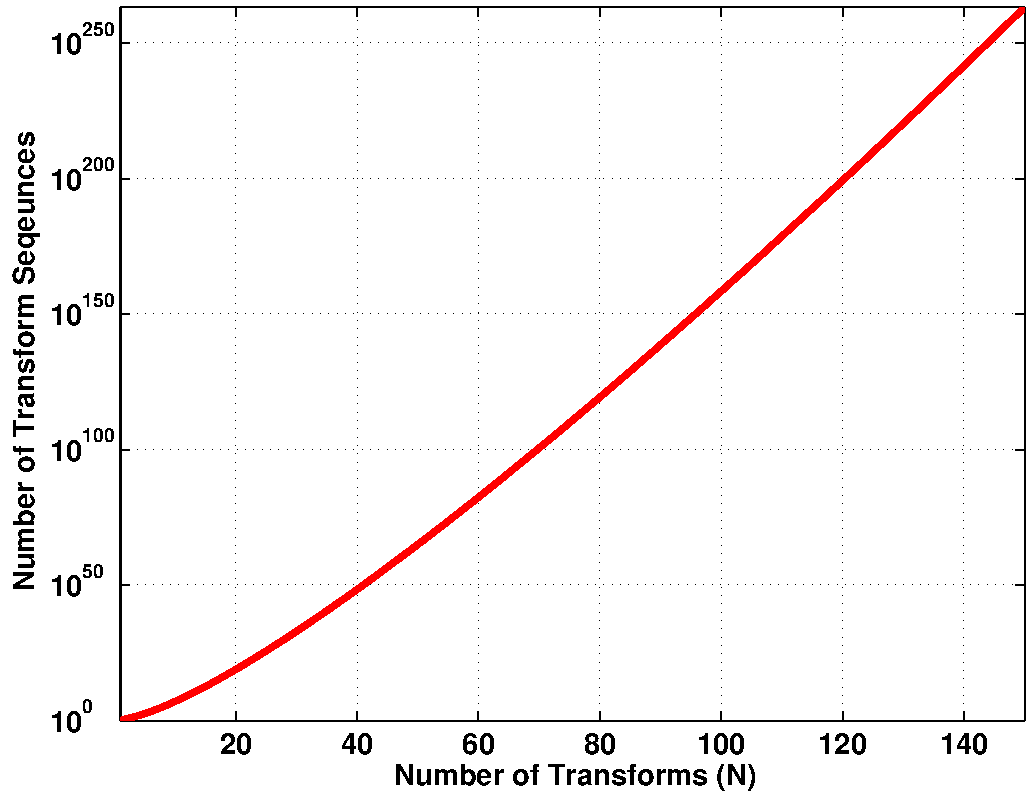
\includegraphics[width=0.35\textwidth]{figs/ss_growth.pdf}
\caption{The number of transform sequences as a function of the number of transforms, assuming no transforms are invalidated and no new transforms are introduced.}
\label{fig:ss_growth}
\end{figure}

In what follows we show how redundancy, transform dynamics, independence, and likelihood can be exploited to enable the practical exploration of the space of transform sequences. We adopt a graph-based representation of the search space where nodes represents the image after a transform sequence, where each transform is a directed link within the graph, and where a transform sequence is a path from the root node (initial image) to a node in the graph, \eg, see Figure~\ref{fig:seq_cgraphs}\textcolor{red}{a}.


%% The construction and traversal of this graph capture the exploration of our search space, namely the space of all transform sequences.  

%% To understand the steps we take to reduce our search space to a manageable size, we first need to define the original size of this space. It is difficult to model the exact size of the space as our search space is dynamic. Some transform sequences will invalidate others shrinking the size of our space, while others introduce new transforms thus expanding our search space. If however, we assume that all transforms are independent, no new transforms are introduced and no old transforms are disqualified, then we can exactly model the size of the space. Given an image with $N$ independent transformations, the size of the search space is defined by all possible permutations of subsets (excluding empty set) of $N$, Equation~\ref{eq:complexity}. We observe the growth of Equation~\ref{eq:complexity} on a log scale, as a function of the number of transforms, $N$, in Figure~\ref{fig:ss_growth}. For example, if $N$ was three, our search space would be defined by fifteen possible transform sequences, $\{(T_1),(T_2),(T_3),(T_1,T_2),(T_2,T_1),(T_1,T_3),(T_3,T_1),(T_2,T_3),\newline(T_3,T_2),(T_1,T_2,T_3),(T_1,T_3,T_2),(T_2,T_1,T_3),(T_2,T_3,T_1),\newline(T_3,T_2,T_1),(T_3,T_1,T_2)\}$. If however we detected a hundred transforms the number of transform sequences to consider would be on the order of $2.5^{158}$! Fortunately, the realistic case does not reach these astronomical estimates for the reasons discussed below. 



%% In what follows, we discuss our efforts for computational reduction for this special case.   

 %% our efforts for computational reduction are not focused on exactly reducing the search space, but on coming up with a tighter and tighter upper bound to Equation~\ref{eq:complexity}. 



%% This represents a very conservative upper bound as we know that at least some subsets of the original set will be dependent and hence some transform sequences will fail to exist in our search space. In regards to the appearance of new transforms, we assume that this number does not exceed the original size $N$. Empirically we have observed this to be true. Furthermore the appearance of new transforms, is usually along paths that invalidate some other transform sequences, so the net effect is our search does not increase in size. 


%% In what follows, our efforts for computational reduction are not focused on exactly reducing the search space, but on coming up with a tighter and tighter upper bound to Equation~\ref{eq:complexity}. 


\noindent\\
{\bf I. Transform Order Redundancy: } Observe that two or more transform sequences may lead to the same result. This was illustrated in Figure~\ref{fig:snake_seq} where applying the two transform sequences $(G_1,L_1,G_2)$ and $(G_2,G_1,L_1)$, illustrated as the red and cyan paths in the search tree of Figure~\ref{fig:seq_cgraphs}\textcolor{red}{a}, lead to the identical result. The recognition that the resulting states, $N_{12}$ and $N_{15}$, are identical implies that any further processing on each of these can be consolidated, thereby reducing the search space. In fact in this example there are additional equivalent states, \eg, resulting from $(G_1,L_1)$ and $(L_1,G_1)$ where $N_6 \equiv N_7$, thereby reducing the number of independent states from 16 to 8, as shown in Figure~\ref{fig:seq_cgraphs}\textcolor{red}{b}.     


%% $N_1 \xrightarrow[]{G_1} N_2 \xrightarrow[]{L_1} N_6$ and $N_1 \xrightarrow[]{L_1} N_3 \xrightarrow[]{G_1} N_7$,

\begin{figure}[ht]
  \centering
  {\footnotesize\textit{\textcolor{black}{a)}}}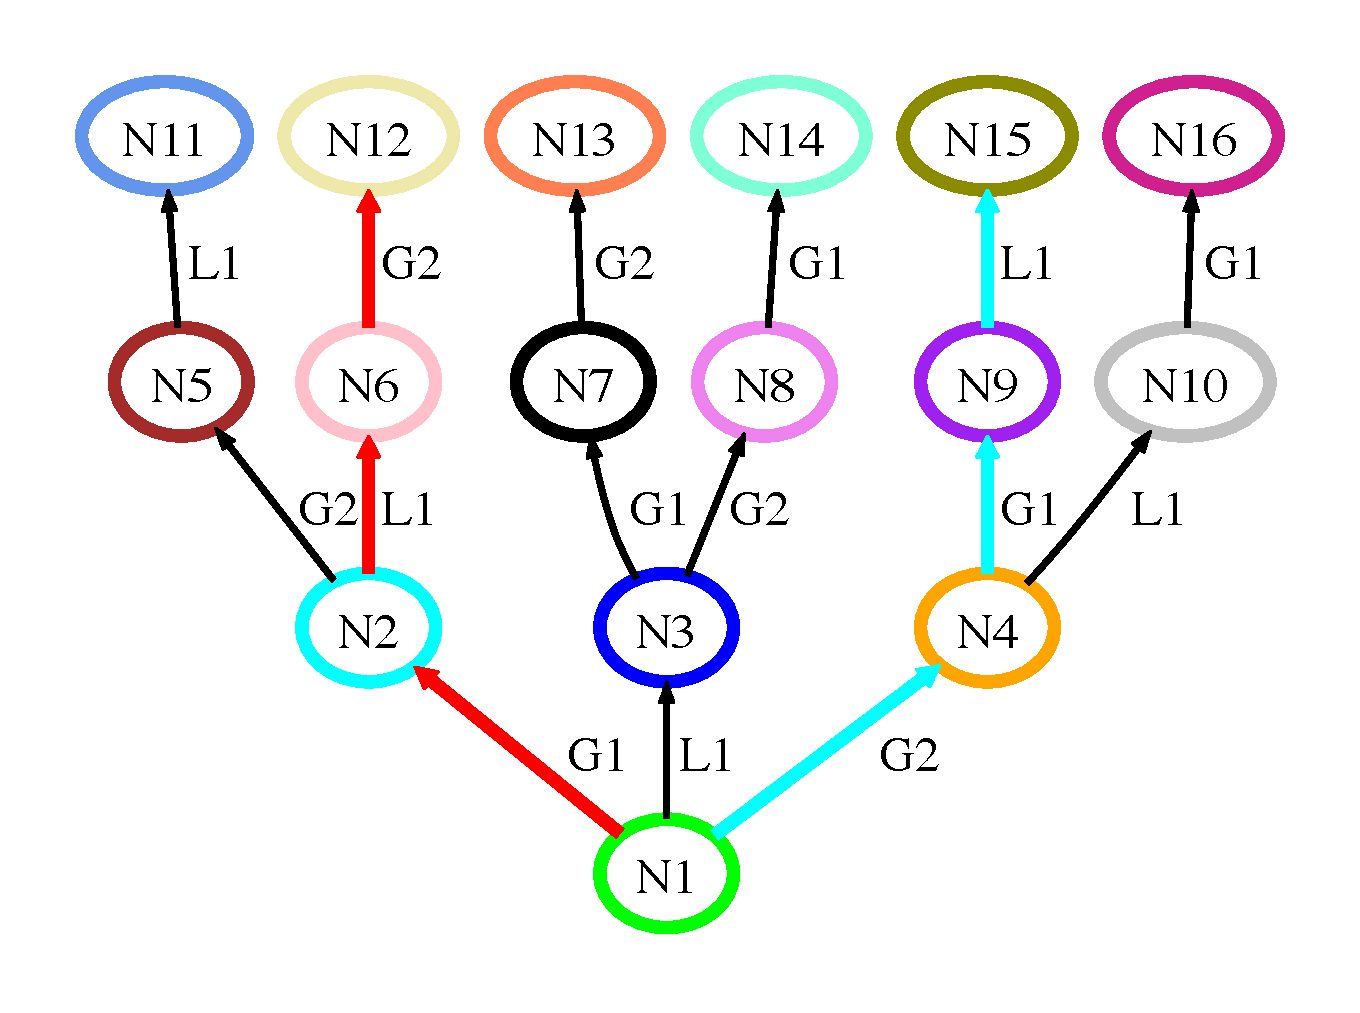
\includegraphics[height=0.22\textwidth]{figs/full_snake_cgraph_no_red.pdf} 
  {\footnotesize\textit{\textcolor{black}{b)}}}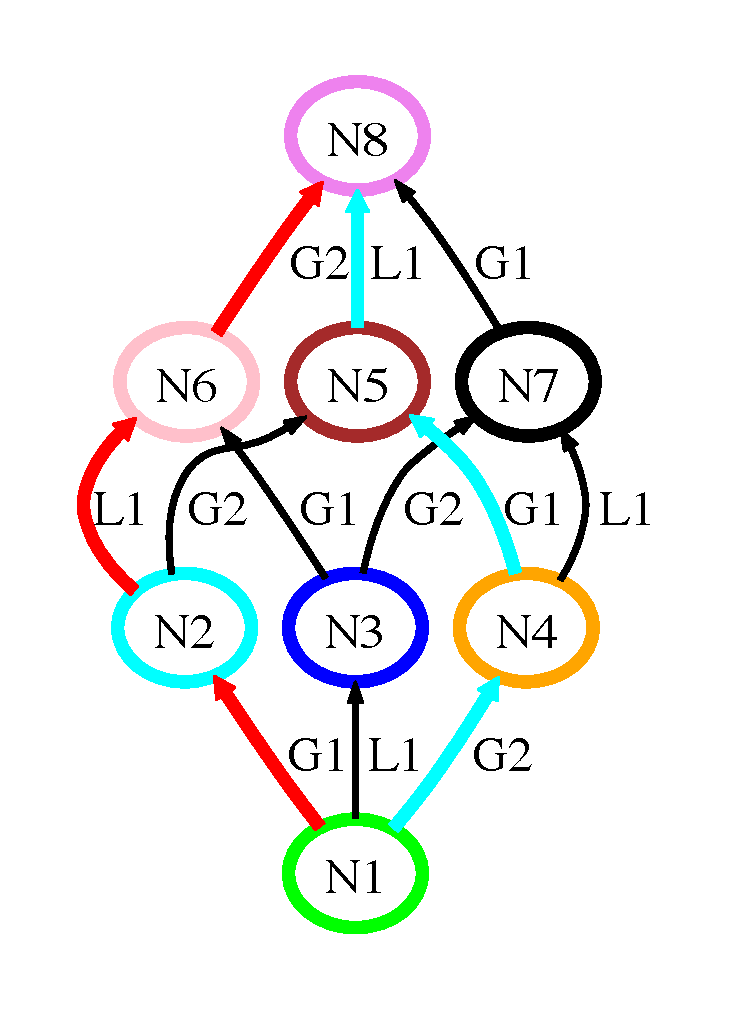
\includegraphics[height=0.22\textwidth]{figs/full_snake_cgraph.pdf} 
 % b)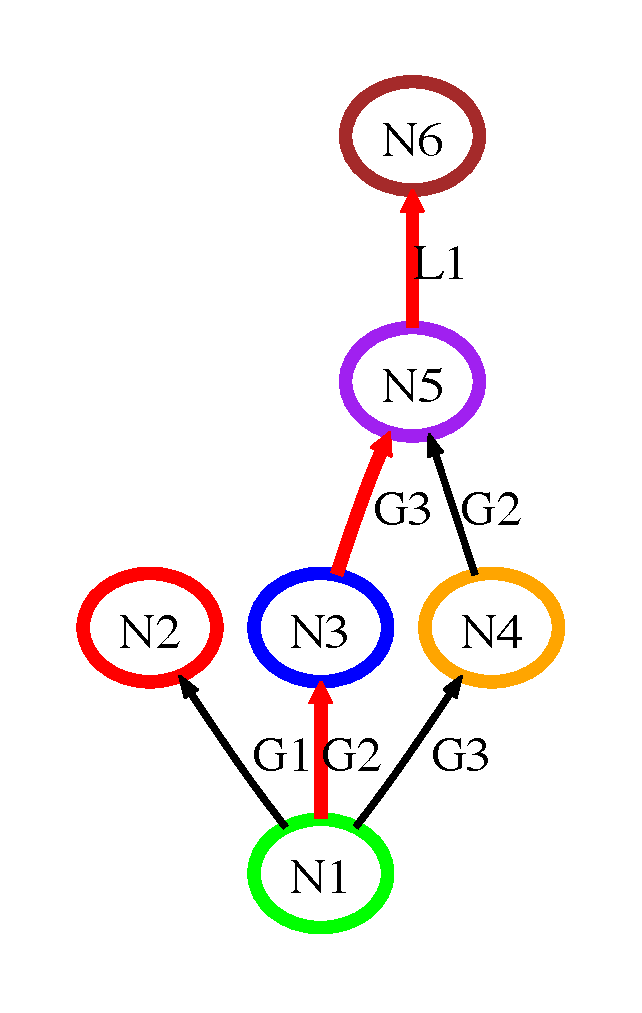
\includegraphics[height=0.25\textwidth]{figs/full_mushroom_cgraph.pdf}
  \caption{a) The search space represented as a tree for Figure~\ref{fig:snake_seq}. The \textcolor{cyan}{cyan} and \textcolor{red}{red} paths in the tree, represent the two redundant paths explored in Figure~\ref{fig:snake_seq}. b) The structure of the search space changes from a tree to a graph as we capture all the inherent redundancies. The same paths are highlighted in the graph structure. }
  \label{fig:seq_cgraphs}
\end{figure}

Many such redundancies arise when the order of application of transforms in a sequence does not affect the final outcome. When all transforms are order independent, the search space is significantly reduced, \ie, 

\begin{equation}
T(N)=\sum_{k=1}^{N}\binom{N}{k}=2^N-1,
\label{eq:complexity2}
\end{equation}

\noindent
which has been plotted in Figure~\ref{fig:ss_growth_redun}. In general, when two transforms do not affect each other, say two gap candidates that do not share the same endpoints, these transforms can be applied in either order leading to the same results. 


\begin{figure}[ht]
\centering
%% \begin{equation}
%% T(N)=\sum_{k=1}^{N}\binom{N}{k}=2^N-1
%% \label{eq:complexity2}
%% \end{equation}
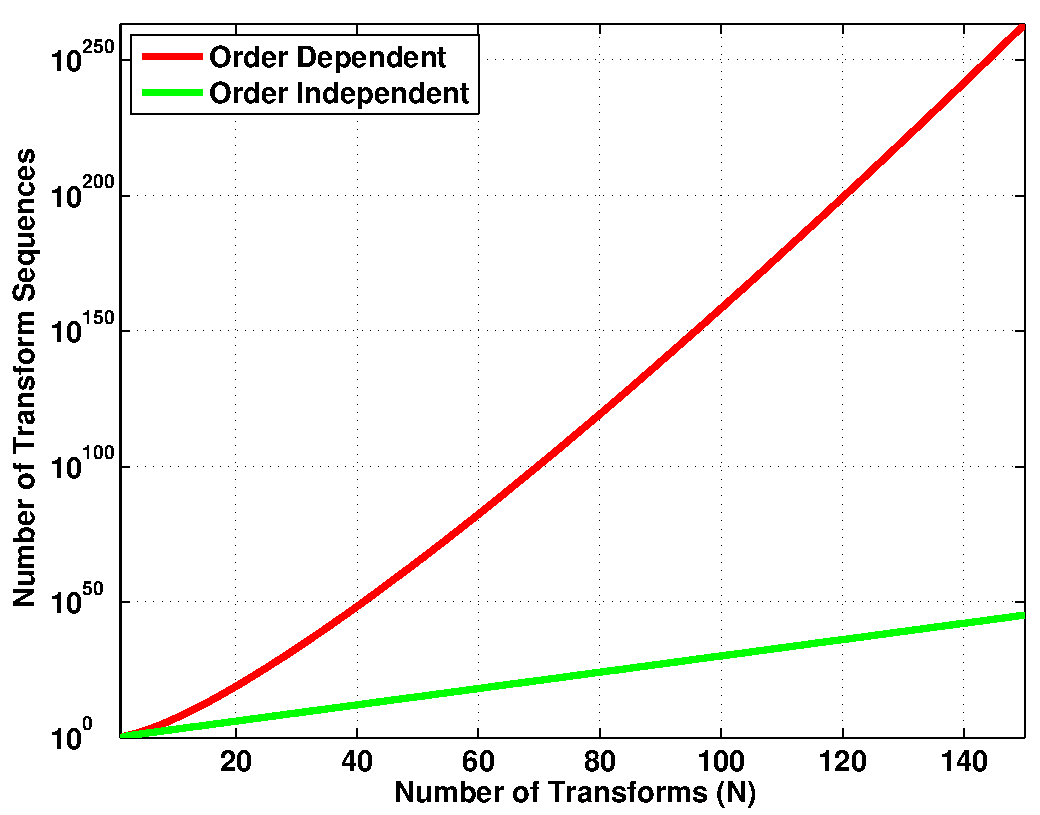
\includegraphics[width=0.35\textwidth]{figs/ss_growth_redun.pdf}
\caption{When transform sequences are invariant to the order of the transforms the search space is significantly reduced.}
\label{fig:ss_growth_redun} 
\end{figure}


\noindent
{\bf II. Transform Independence and Clustering: } Define a pair of transforms as independent when the application of one transform does not invalidate the applicability of the other transform nor affect its outcome, and vice-versa  {\footnotesize\footnote{In general, independence is a symmetric relationship: if $T_1$ does not invalidate nor affect the outcome of $T_2$, then $T_2$ also does not invalidate nor affect the outcome of $T_1$. [Add proof statement] }}. Define two sets of transforms ${\cal T}=\{T_1,T_2,...,T_N\}$ and $\overline{\cal T}=\{\overline{T}_1,\overline{T}_2,...,\overline{T}_N\}$ as independent when any pair of transforms $T_i$ and $\overline{T}_j$ where $i=1,2,...,N,j=1,2,...,M$, is independent, Figure~\ref{fig:cluster_sets}\textcolor{red}{a}. This typically happens often when the transforms in the set ${\cal T}$ are spatially distinct from the transforms in the set $\overline{\cal T}$. Figure~\ref{fig:indep} shows two examples, the flower and the horse image in (a) and (b) respectively, where the location of each transform is indicated by a blue dot, in Figure~\ref{fig:indep}\textcolor{red}{(c,d)}. All pairs of transforms where one transform invalidates another are connected by a red line, Figure~\ref{fig:indep}\textcolor{red}{(e,f)}. Observe that each transform is typically independent with all other transforms, except for a few in its own neighborhood. 

\begin{figure}[!ht]
\centering
{\footnotesize\textit{a)}}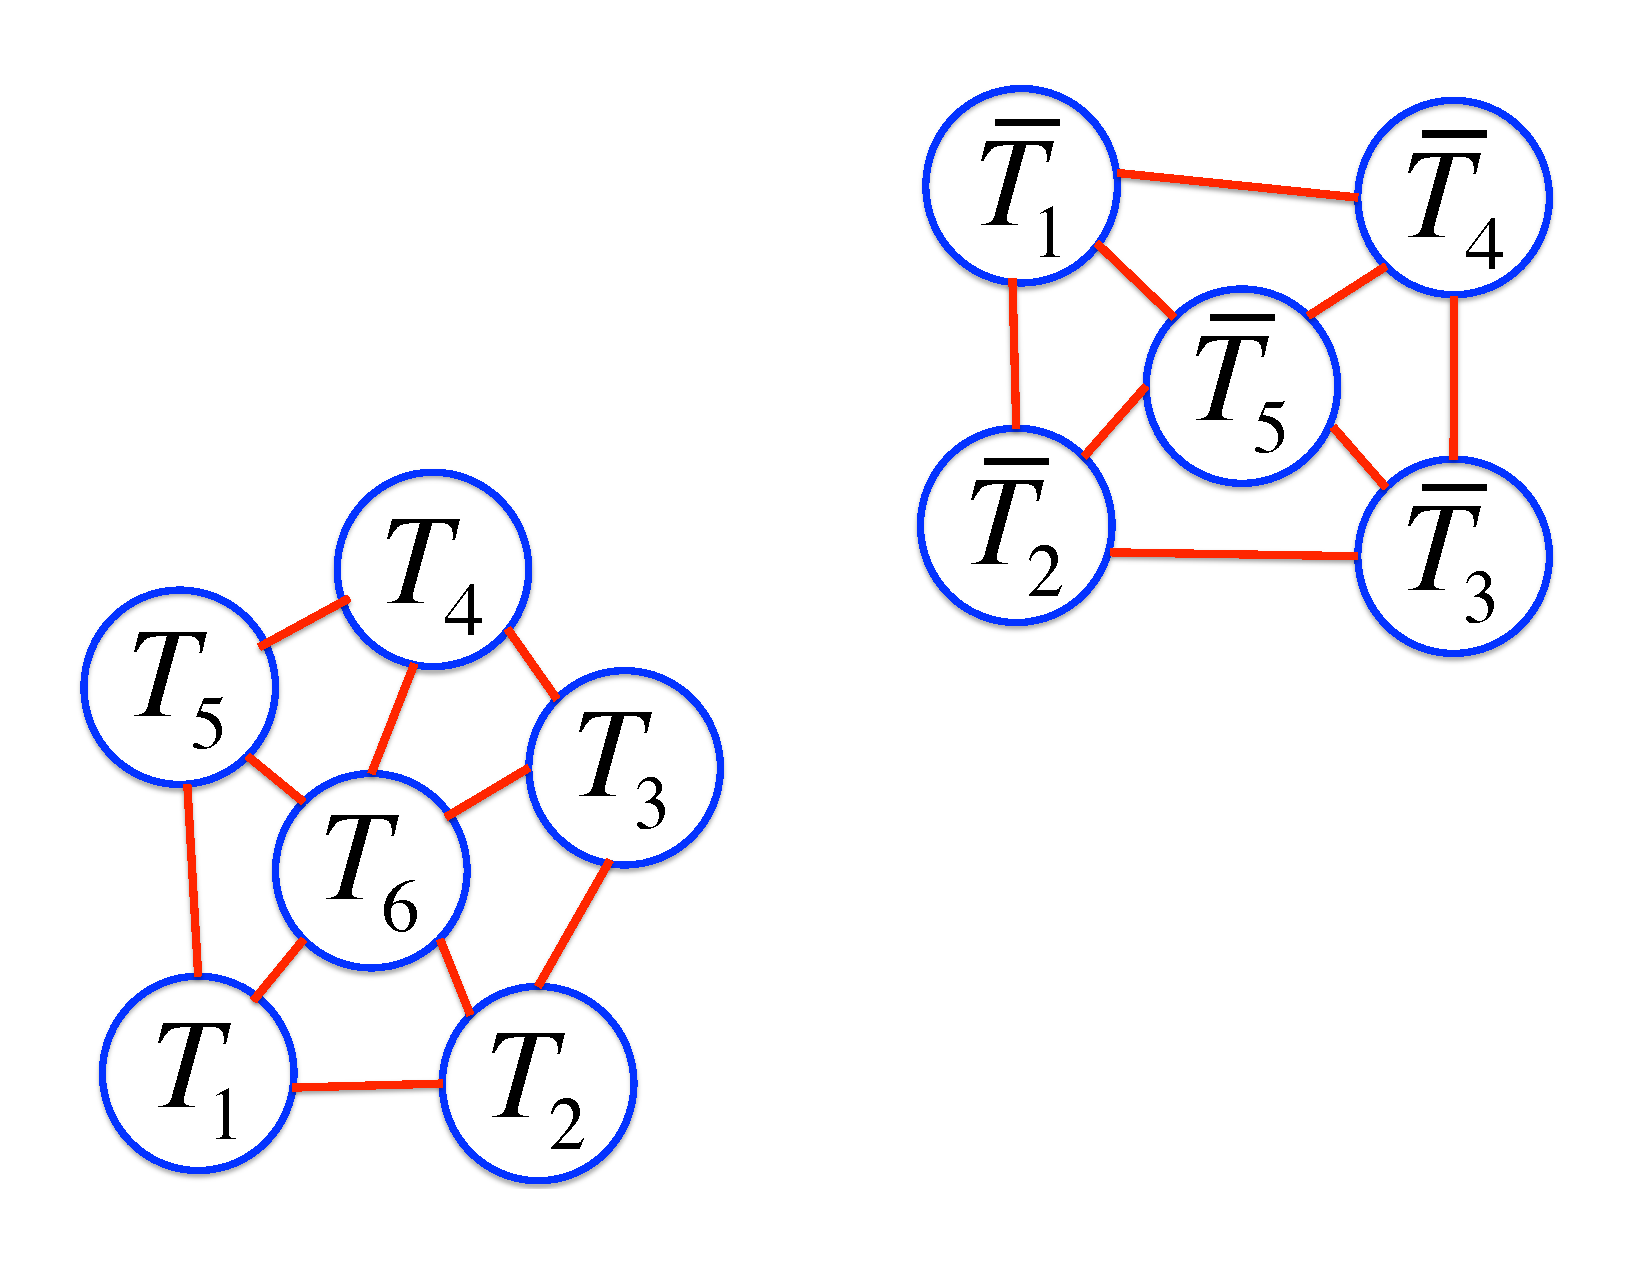
\includegraphics[width=0.25\linewidth]{figs/clusters.pdf}
{\footnotesize\textit{b)}}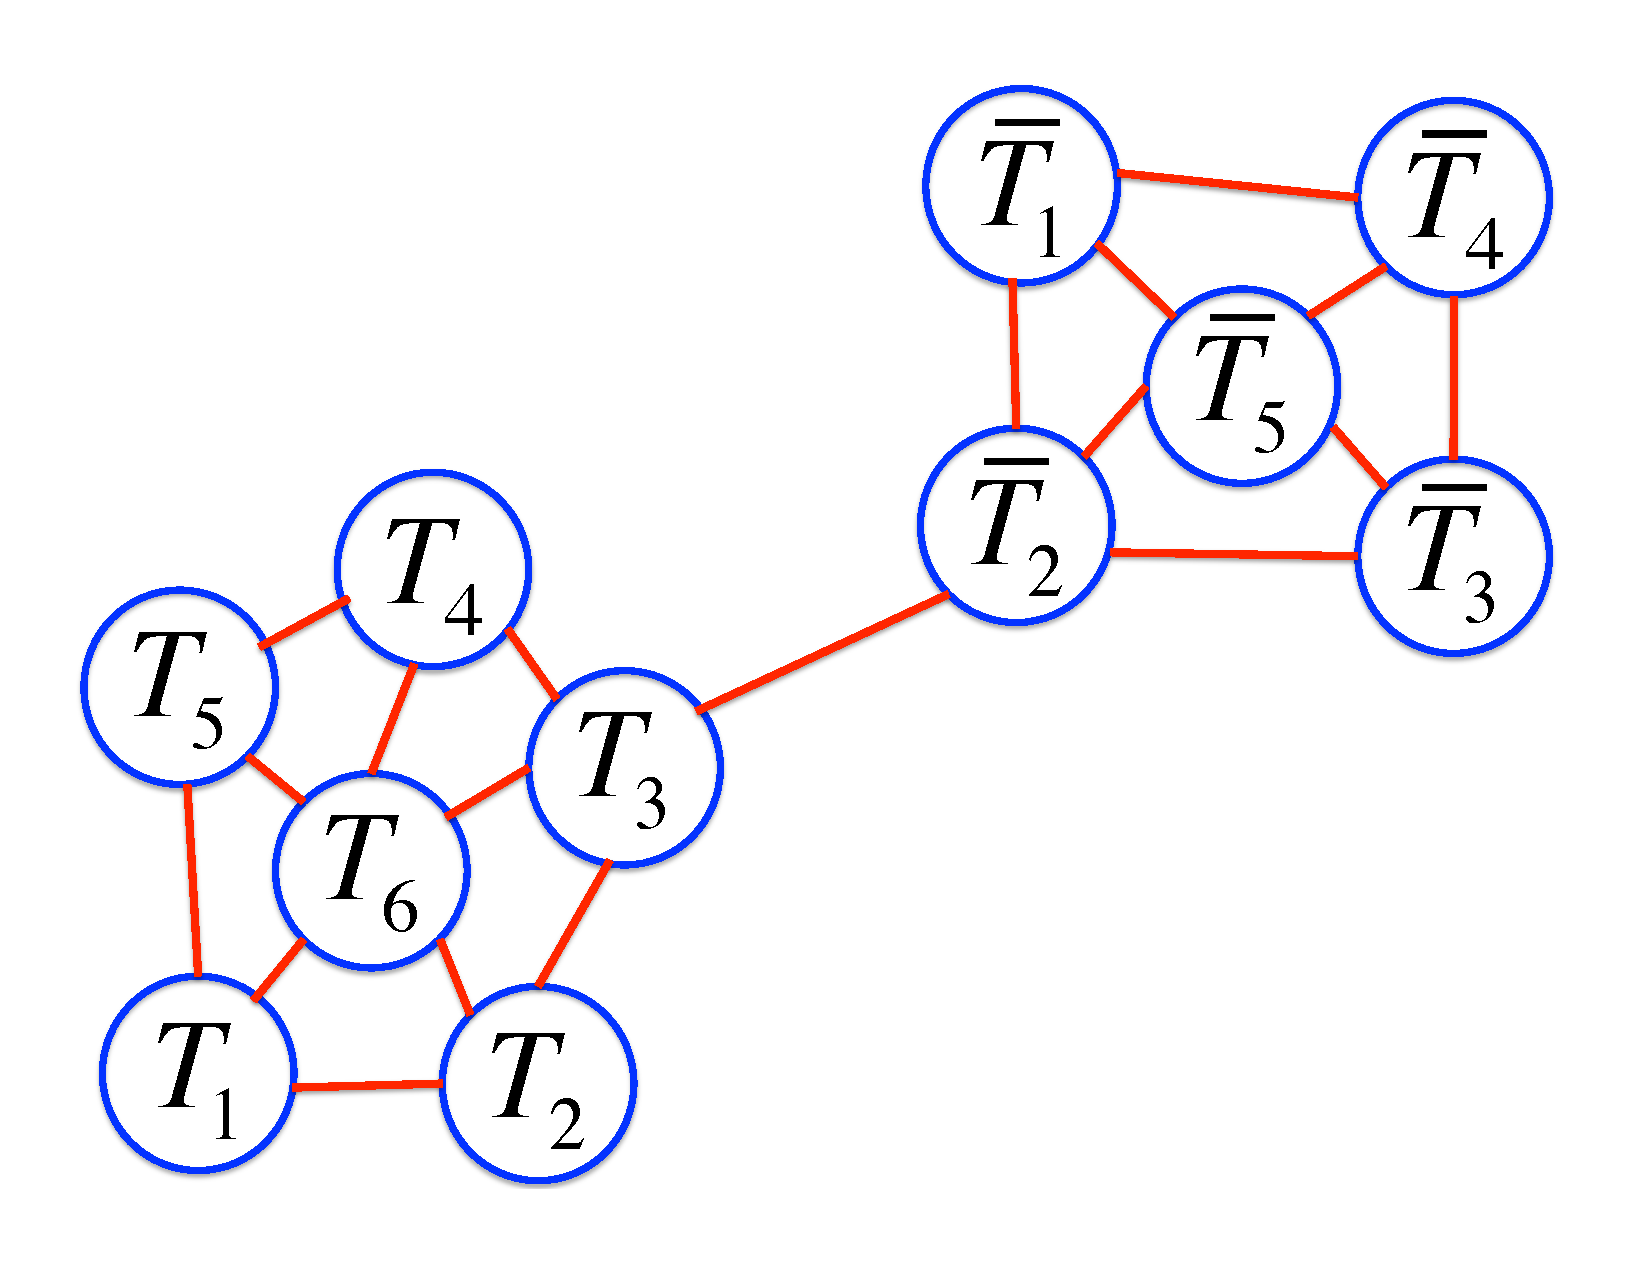
\includegraphics[width=0.25\linewidth]{figs/clusters_depend.pdf}
\caption{a) The search space of two independent sets of transforms, say ${\cal T}=\{T_1,T_2,T_3,T_4,T_5,T_6\}$ and $\overline{\cal T}=\{\overline{T}_1,\overline{T}_2,\overline{T}_3,\overline{T}_4,\overline{T}_5\}$ can be independently explored and then combined. (b) Introducing a limited degree of dependency implies reduction in the number of transform sequences, \ie, any transform containing $T_3$ cannot be followed by $\overline{T}_2$, or it can be followed by with an outcome dependent on the presence of $T_3$.}
\label{fig:cluster_sets}
%\vspace{-0.751cm}
\end{figure}


\begin{figure}[!ht]
\centering
%\setlength{\tabcolsep}{1pt}
{\footnotesize\textit{a}}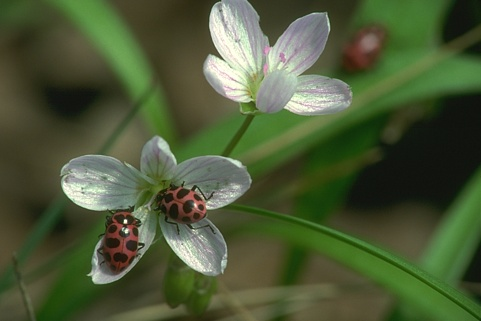
\includegraphics[width=0.35\linewidth]{figs/35008_00.png}
{\footnotesize\textit{b}}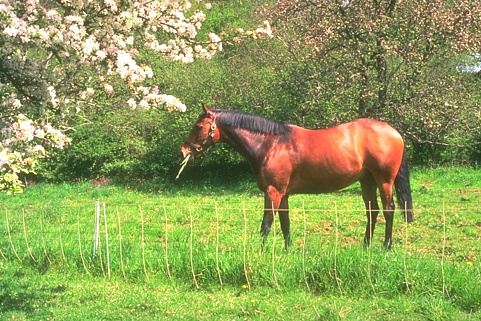
\includegraphics[width=0.35\linewidth]{figs/291000_00.png}
{\footnotesize\textit{c}}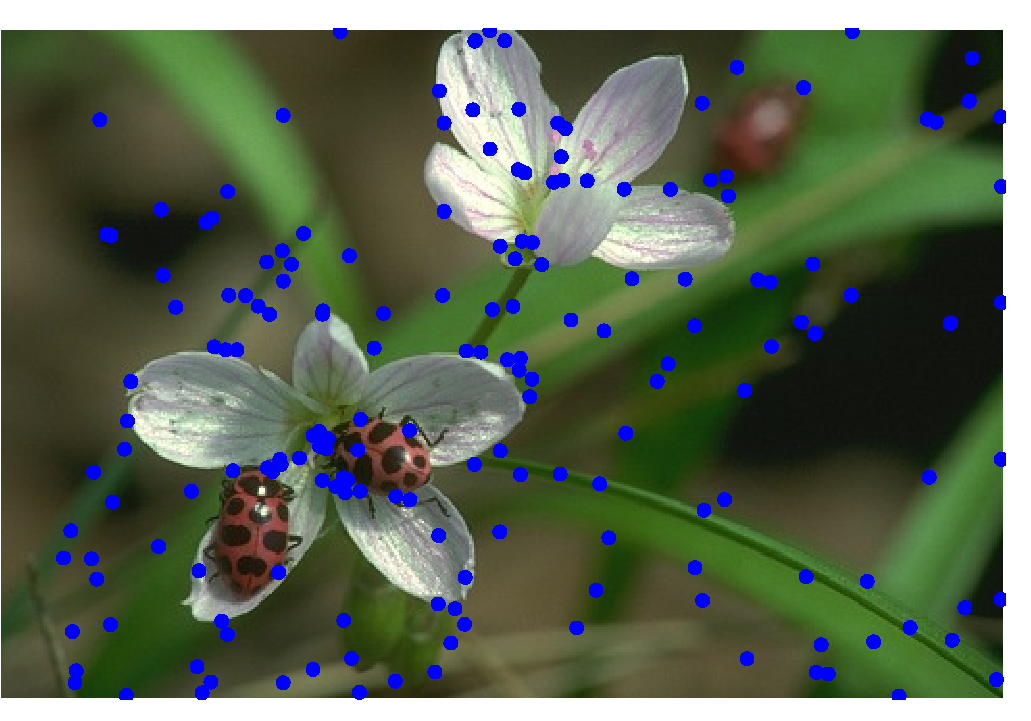
\includegraphics[width=0.35\linewidth]{figs/35008_transforms.pdf}
{\footnotesize\textit{d}}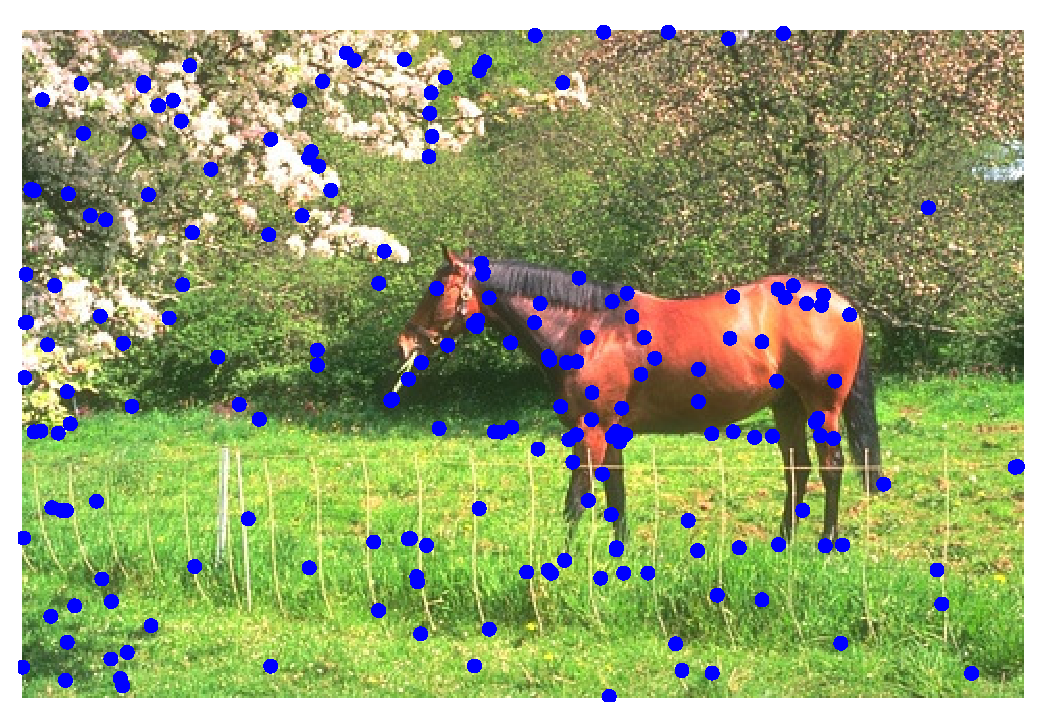
\includegraphics[width=0.35\linewidth]{figs/291000_transforms.pdf}
{\footnotesize\textit{e}}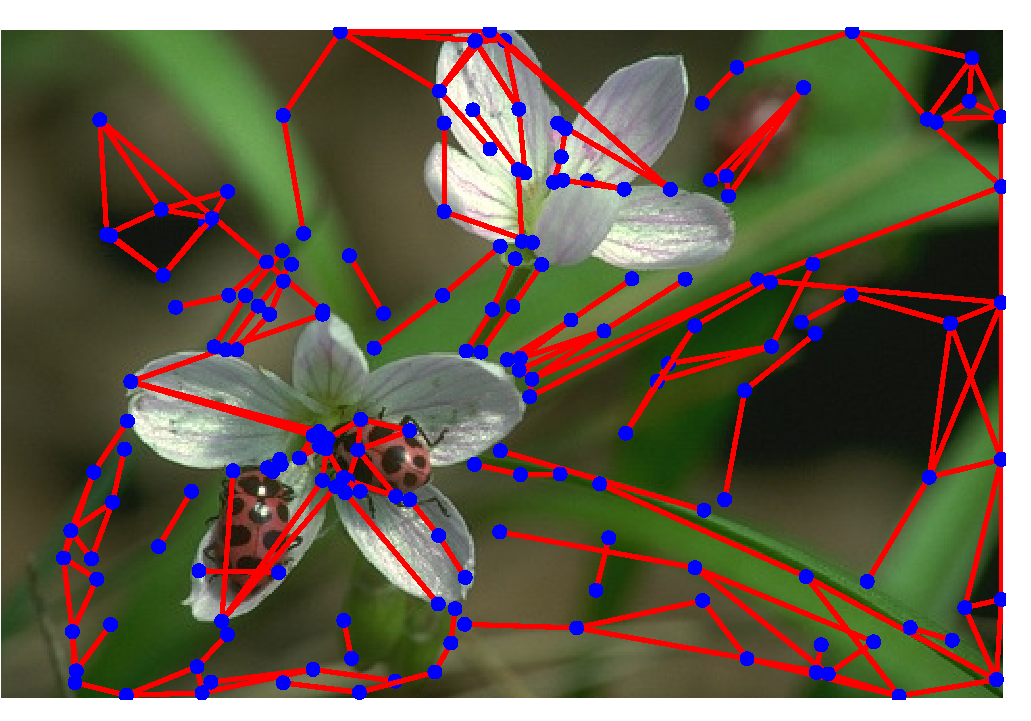
\includegraphics[width=0.35\linewidth]{figs/35008_depend_graph.pdf}
{\footnotesize\textit{f}}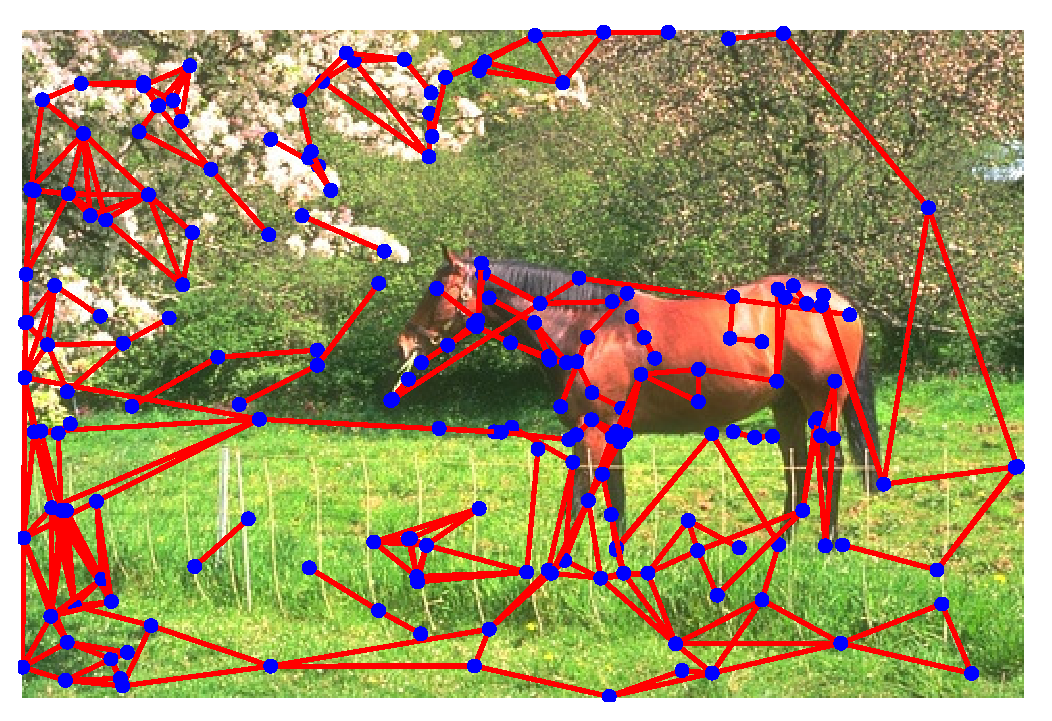
\includegraphics[width=0.35\linewidth]{figs/291000_depend_graph.pdf}
\caption{Example images, a-b), and a set of detected transforms shown respectively in c-d). Each blue dot represents a transform and we can observe the symmetric pairwise relationship between transforms in e-f). Each red-line indicates that the application of either transform invalidates the other. }
\label{fig:indep}
%\vspace{-0.751cm}
\end{figure}



Consider now a set of transforms that can be divided into two independent sets of transforms ${\cal T}$ and $\overline{\cal T}$ as described above. Any transform sequence can then be seen as two interleaved transform subsequences, one subsequence made from transforms in ${\cal T}$ and one subsequence from transforms in $\overline{\cal T}$. This implies that the space of the two subsequences can be explored independently and then joined \eg, the transform sequence $(T_3,\overline{T}_2,T_1,\overline{T}_4,\overline{T}_5,T_4,T_6)$ can be thought of as the two transform sequences $(T_3,T_1,T_4,T_6)$ and $(\overline{T}_2,\overline{T}_4,\overline{T}_5)$ when applied independently in sequence. This implies a tremendous reduction in the search space: if a set of $N$ transforms can thus be divided into two equal independent sets of $\floor*{\frac{N}{2}}$ transforms each, then the search space reduces from $(2^N-1)$ to $2(2^{\floor*{\frac{N}{2}}}-1)$. The reduction corresponding to an organization into 10 independent sets of transforms is even more pronounced, from $2^N-1$ to $10(10^{\floor*{\frac{N}{10}}}-1)$: for $N \equiv 100$ this amounts to a reduction from $10^{30}$ nodes to $10^5$ nodes! Formally, if the set of transforms can be divided into $M$ independent sets of transforms, the search space size can by captured by 

\begin{equation}
T(N)=M\sum_{i=k}^{\floor*{\frac{N}{M}}}\binom{\floor*{\frac{N}{M}}}{k}=M(2^{\floor*{\frac{N}{M}}}-1),
\label{eq:complexity3}
\end{equation}

\noindent
as illustrated in Figure~\ref{fig:frag_growth_redun}.

\begin{figure}[ht]
\centering
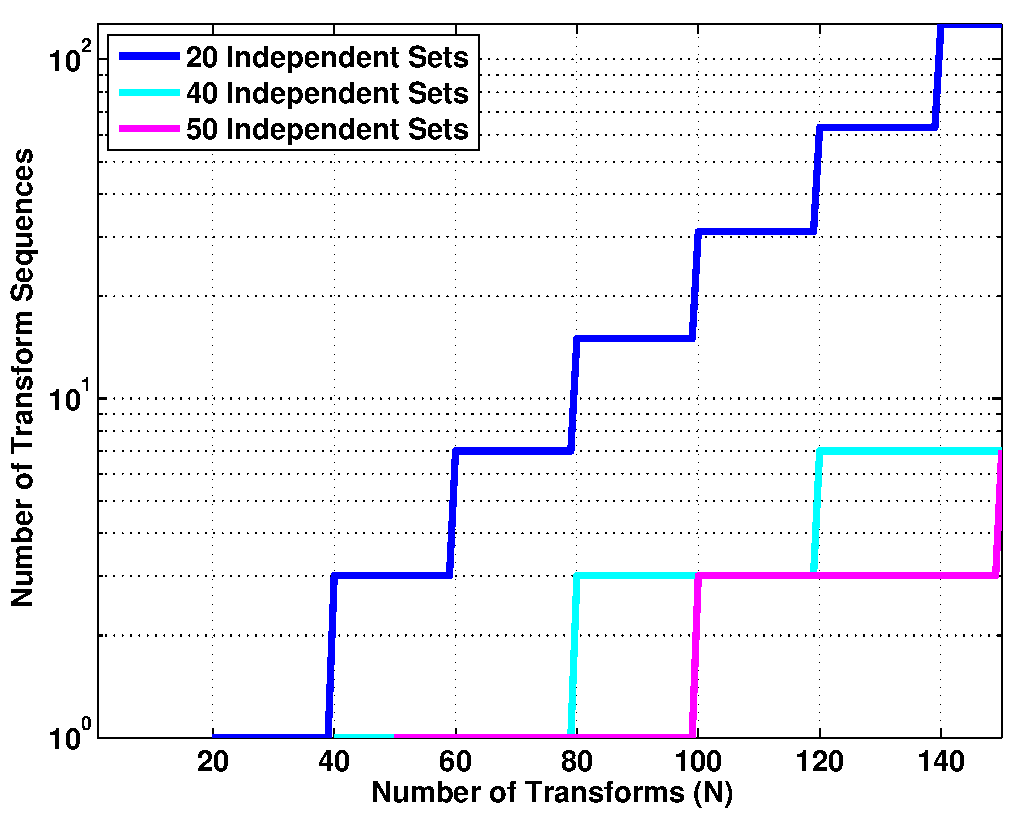
\includegraphics[width=0.35\textwidth]{figs/frag_growth.pdf}
\caption{Dividing the set of transforms into $M$ independent sets reduces the search space significantly as shown for $M=20,40,50$.}
\label{fig:frag_growth_redun} 
\end{figure}

%% \begin{figure*}[!ht]
%% \centering
%% %\setlength{\tabcolsep}{1pt}
%% {\footnotesize\textit{a)}}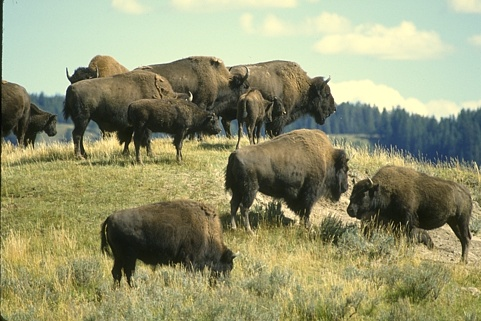
\includegraphics[width=0.30\linewidth]{figs/38092_00.png}
%% {\footnotesize\textit{b)}}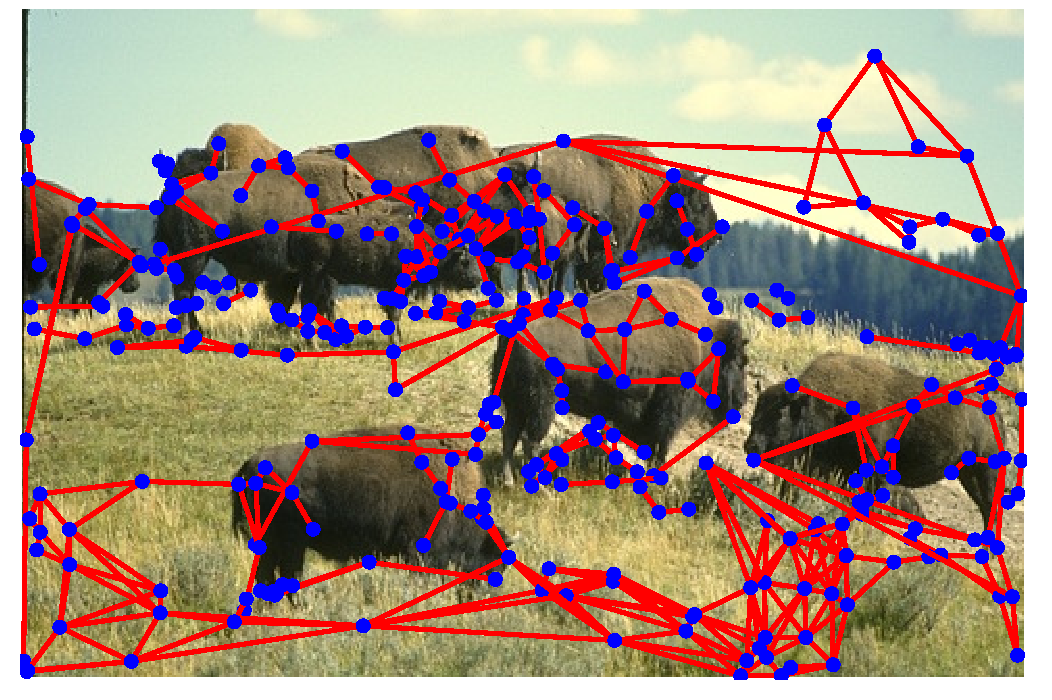
\includegraphics[width=0.30\linewidth]{figs/38092_depend_graph.pdf}
%% {\footnotesize\textit{c)}}
\includegraphics[width=0.30\linewidth]{figs/insert.png}
%% {\footnotesize\textit{d}}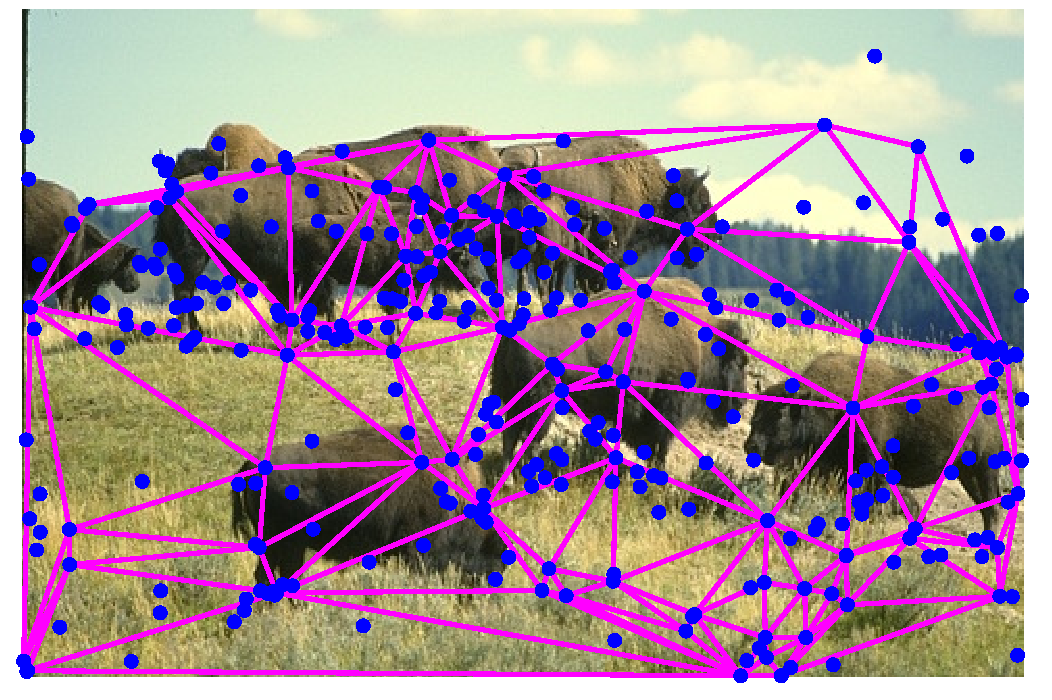
\includegraphics[width=0.30\linewidth]{figs/38092_dt.pdf}
%% {\footnotesize\textit{e}}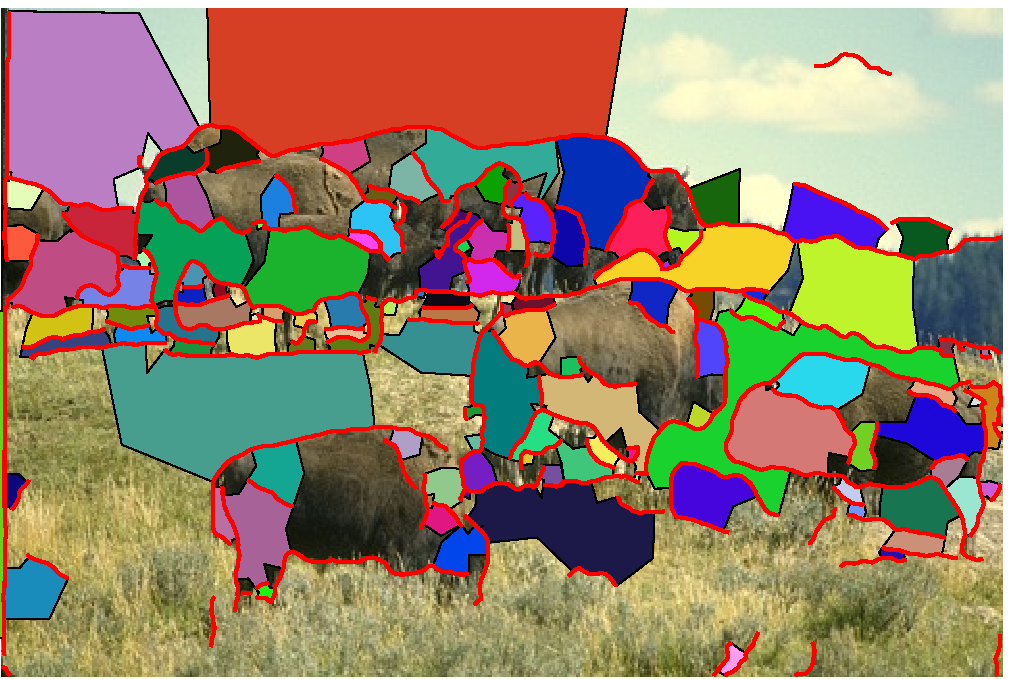
\includegraphics[width=0.30\linewidth]{figs/38092_00_mvf_frags.pdf}
%% {\footnotesize\textit{f}}
\includegraphics[width=0.30\linewidth]{figs/insert.png}
%% \caption{a) Image and the pairwise relationship (b) between a set of detected transforms. Each blue dot represents a transform and each red-line indicates the application of either transform invalidates the other. c) Clustering by partitioning the image into quadrants and d) clustering by approximating the location of transforms by a delaunary triangulation. e-f) Seed MVF's and their transforms they indexed. The transforms indexed are color-coded.   }
%% \label{fig:cluster_schemes}
%% %\vspace{-0.751cm}
%% \end{figure*}

The more realistic case, are more like the examples shown in Figure~\ref{fig:indep}\textcolor{red}{(e,f)}; these transforms include some independent sets, but predominantly any spatial grouping of transforms into two adjacent sets requires a limited dependency between the two. The effect of this dependency can be illustrated by introducing a dependent relationship between nodes $T_3$ and $\overline{T}_2$ in Figure~\ref{fig:cluster_sets}\textcolor{red}{a}, as shown in Figure~\ref{fig:cluster_sets}\textcolor{red}{b}. For the majority of transform sequences, specifically those which do not contain both $T_3$ and $\overline{T}_2$, the situation is handled exactly as the situation before, \ie, by exploring subsequences from ${\cal T}$ and $\overline{\cal T}$ and combining them. For those transform sequences that contain both $T_3$ and $\overline{T}_2$, the presence of one of these transforms affects the outcome of the other: if the application of $T_3$ invalidates $\overline{T}_2$, the search space is in fact reduced because in combining the two the independently formed subsequences from ${\cal T}$ and $\overline{\cal T}$, those where $\overline{T}_2$ follows $T_3$, are simply discarded. A similar situation holds when the application of $\overline{T}_2$ invalidates the application of $T_3$. On the other hand, if the application of $T_3$ simply affects the outcome of $T_2$ then the two independently formed subsequences cannot simply be combined. For example the sequence $(T_9,\overline{T}_6,T_3,T_2,\overline{T}_2,\overline{T}_4,T_5,\overline{T}_7)$ can no longer be a combination of $(T_9,T_3,T_2,T_5)$ and $(\overline{T}_6,\overline{T}_2,\overline{T}_4,\overline{T}_7)$ applied independently, since the application of $\overline{T}_2$ requires knowledge of the application of $T_3$ if $T_3$ has preceded it. Rather, the sequence  $(T_9,T_3,T_2,T_5)$ needs to be augmented by additional transforms to explore $(T_9,\overline{T}_6,T_3,T_2,\overline{T}_2,\overline{T}_4,T_5,\overline{T}_7)$. This is a slight addition to the overall cost as compared to considering two sets of completely independent transforms, but the cost is a at least partially offset by discarding some impossible transform sequences. Thus two set of transforms which are generally independent except for a limited form of dependence can roughly be treated as two independent sets of transforms for the purpose of search space analysis, and we can safely rely on the tremendous advantage of considering clusters of transform independently at first and then combining the results. 

\begin{figure*}[!ht]
  \centering
\setlength{\tabcolsep}{1pt}
{\footnotesize\textit{a}}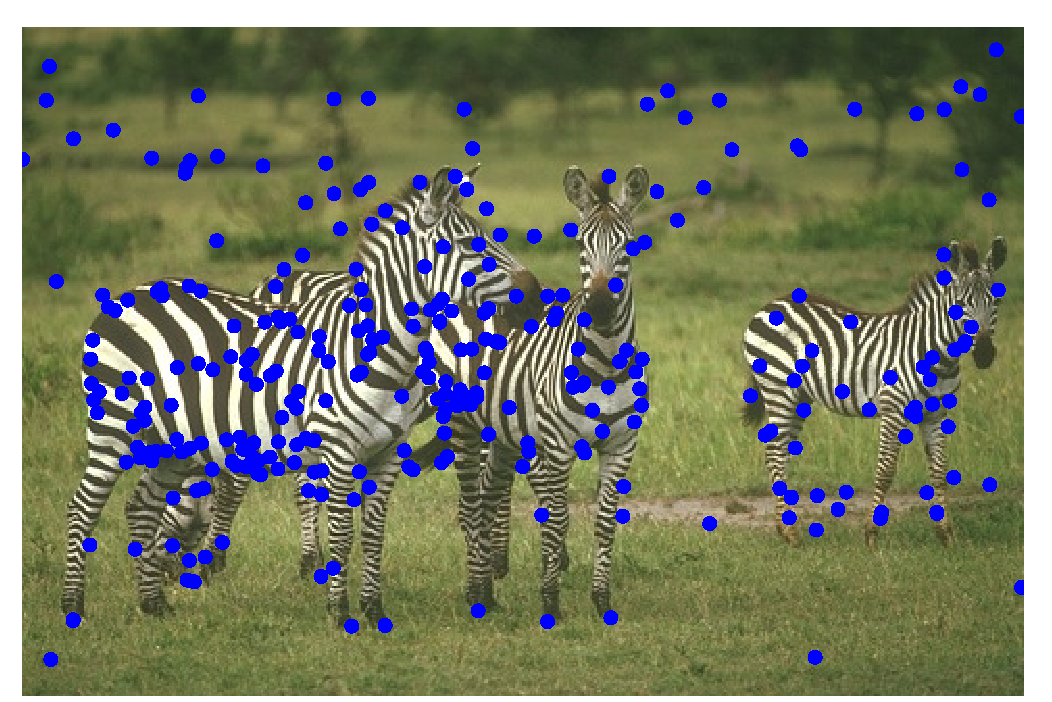
\includegraphics[width=0.32\linewidth]{figs/zebra_transforms.pdf}
{\footnotesize\textit{b}}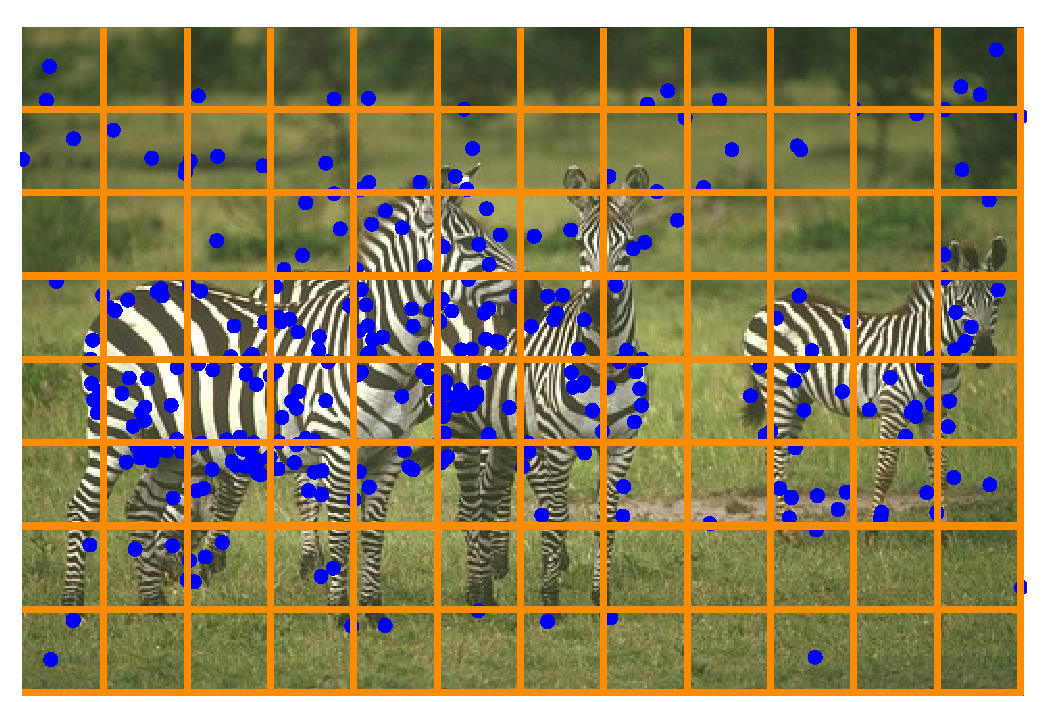
\includegraphics[width=0.32\linewidth]{figs/zebra_grid.pdf}
{\footnotesize\textit{c}} 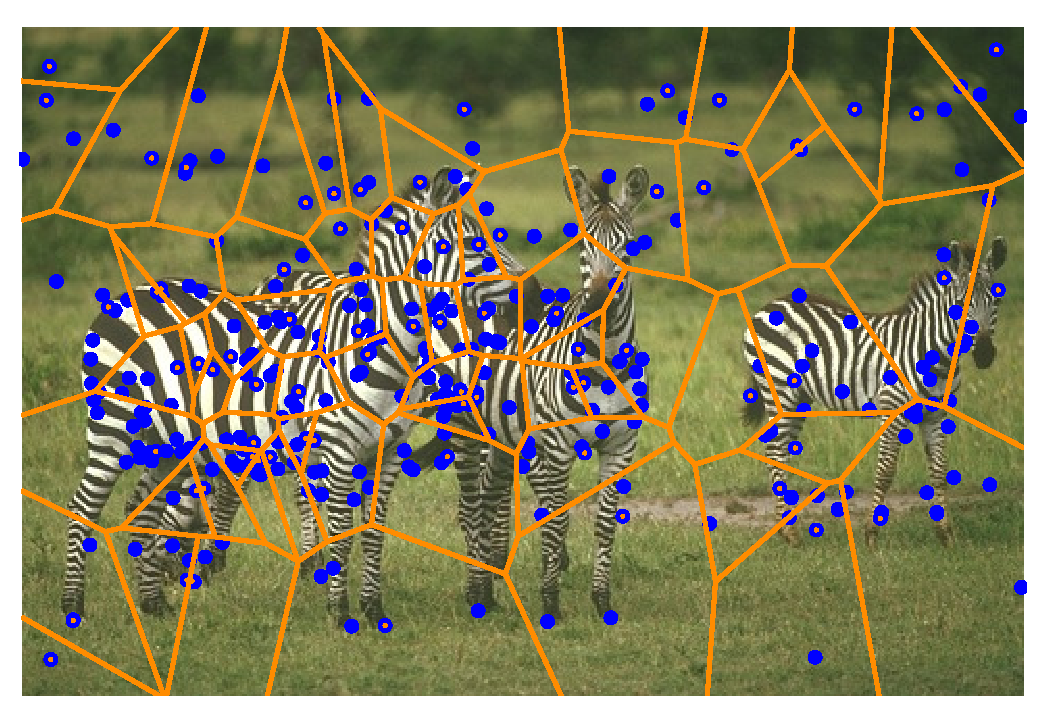
\includegraphics[width=0.31\linewidth]{figs/zebra_voronoi.pdf}
{\footnotesize\textit{d}} 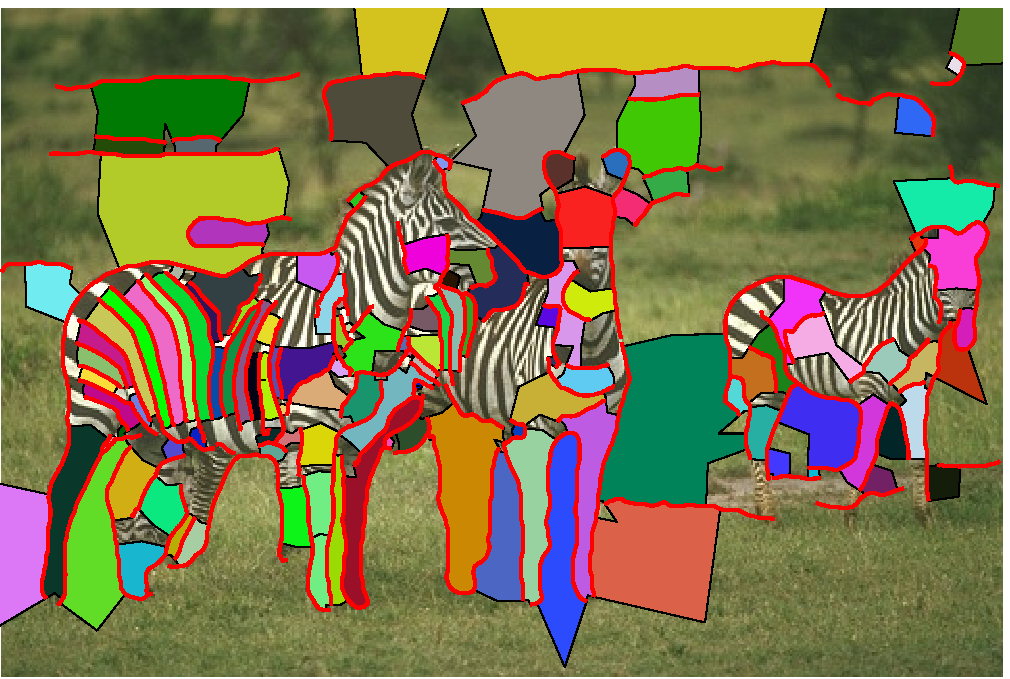
\includegraphics[width=0.31\linewidth]{figs/253027_00_start_mvf_frags.pdf}
%{\footnotesize\textit{d}}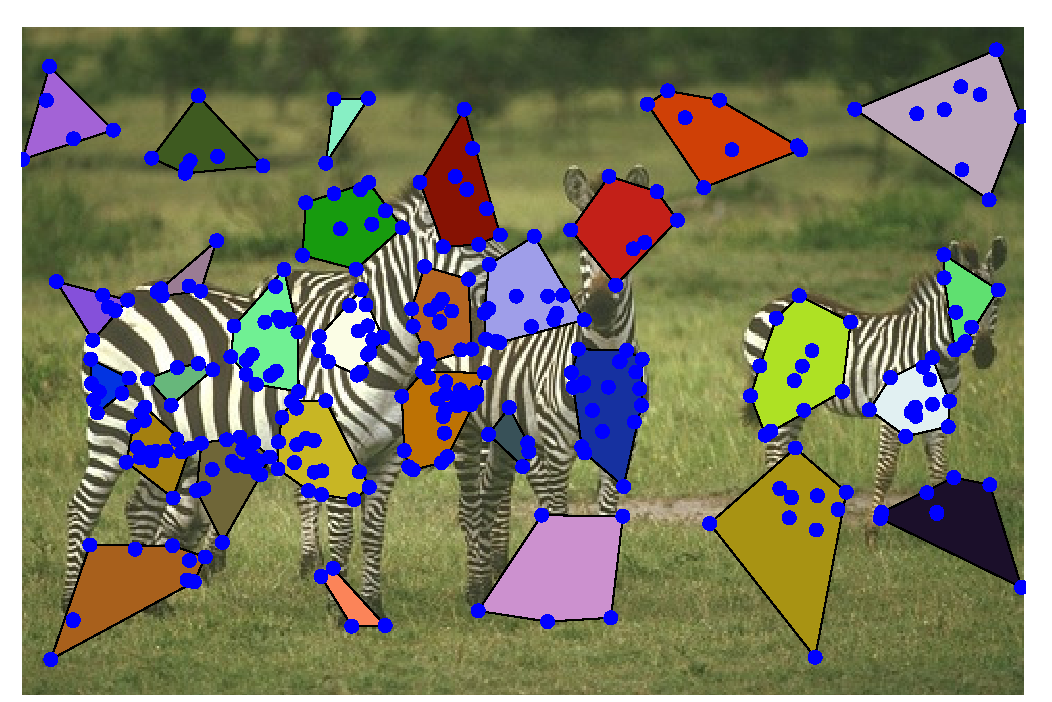
\includegraphics[width=0.31\linewidth]{figs/zebra_k_clustering.pdf}
{\footnotesize\textit{e}} 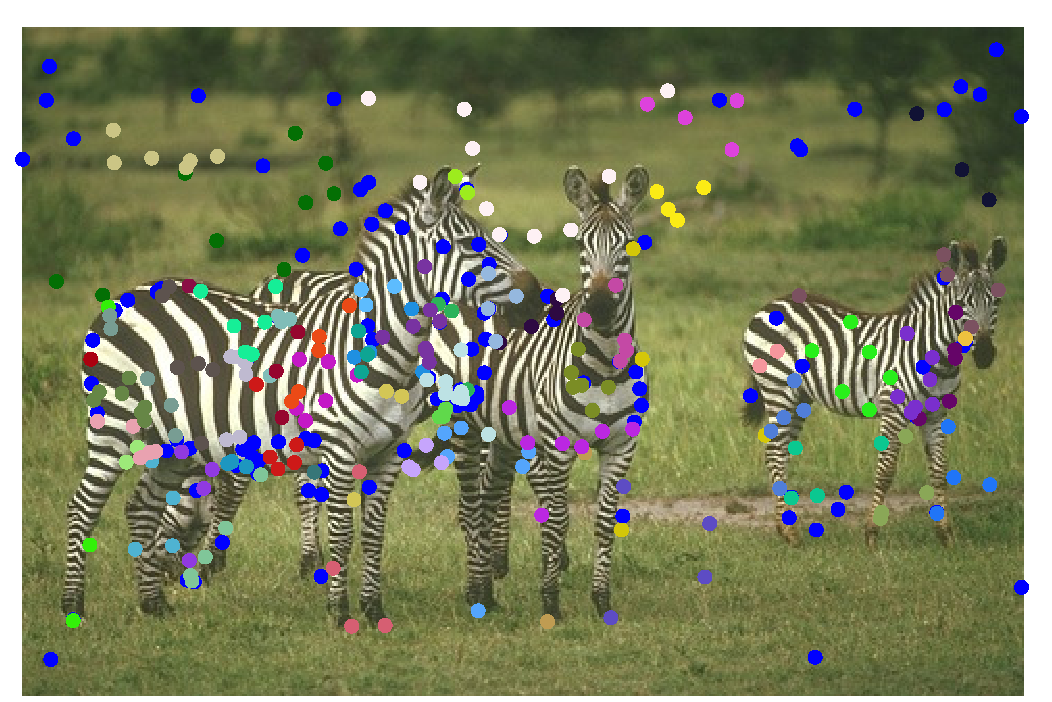
\includegraphics[width=0.31\linewidth]{figs/zebra_frag_clusters.pdf}
{\footnotesize\textit{f}} 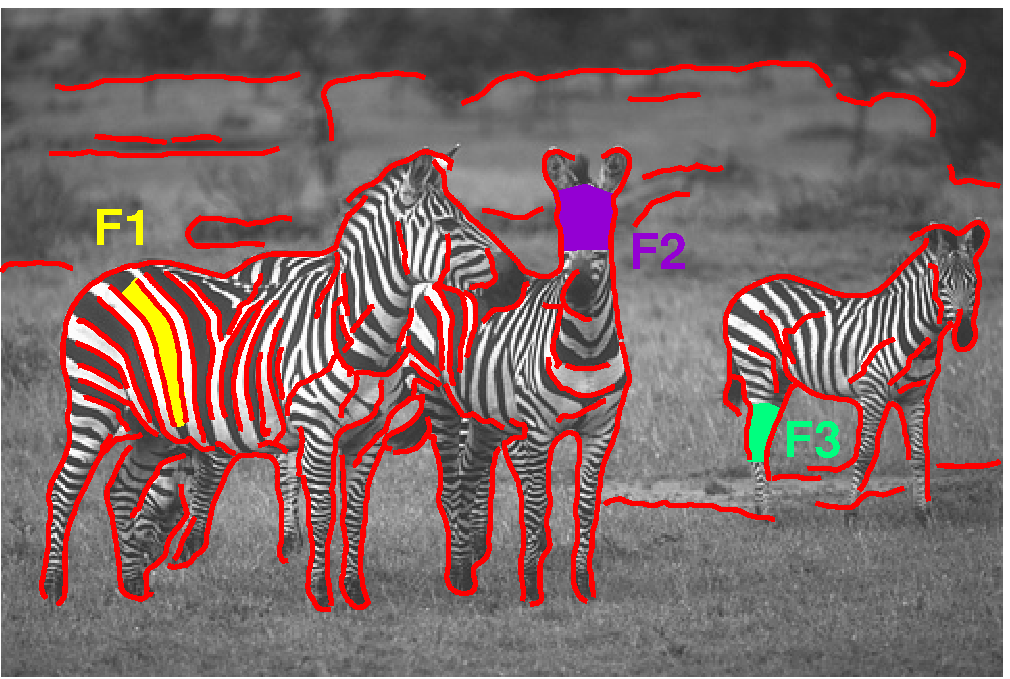
\includegraphics[width=0.31\linewidth]{figs/zebra_frag_start.pdf}
\begin{tabular}{ccc}
{\footnotesize\textit{g}}\raisebox{0.25\height}{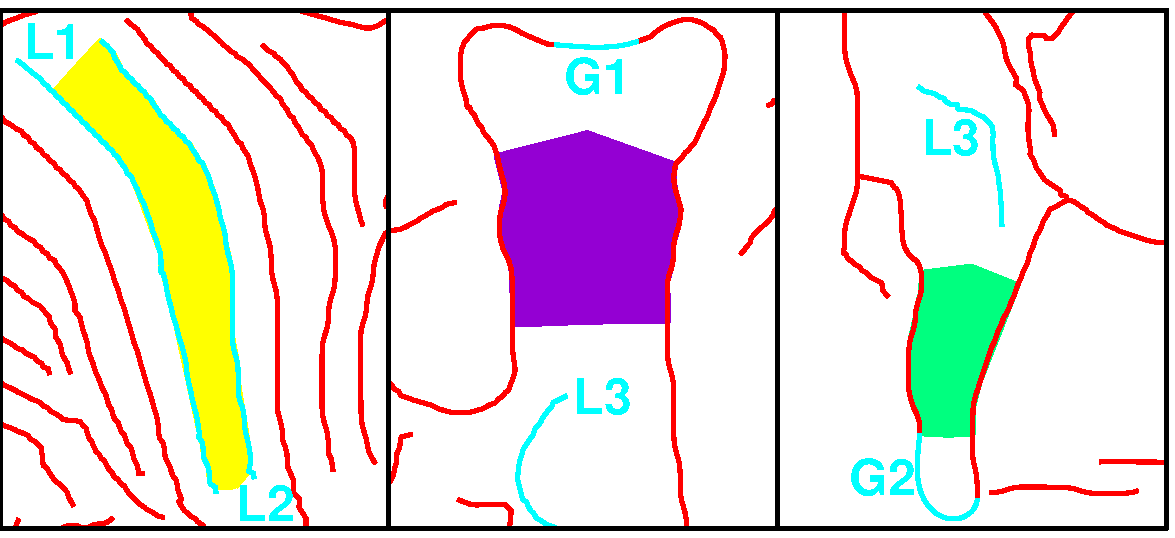
\includegraphics[width=0.32\linewidth]{figs/zebra_frag_index.pdf}} &
{\footnotesize\textit{h}} 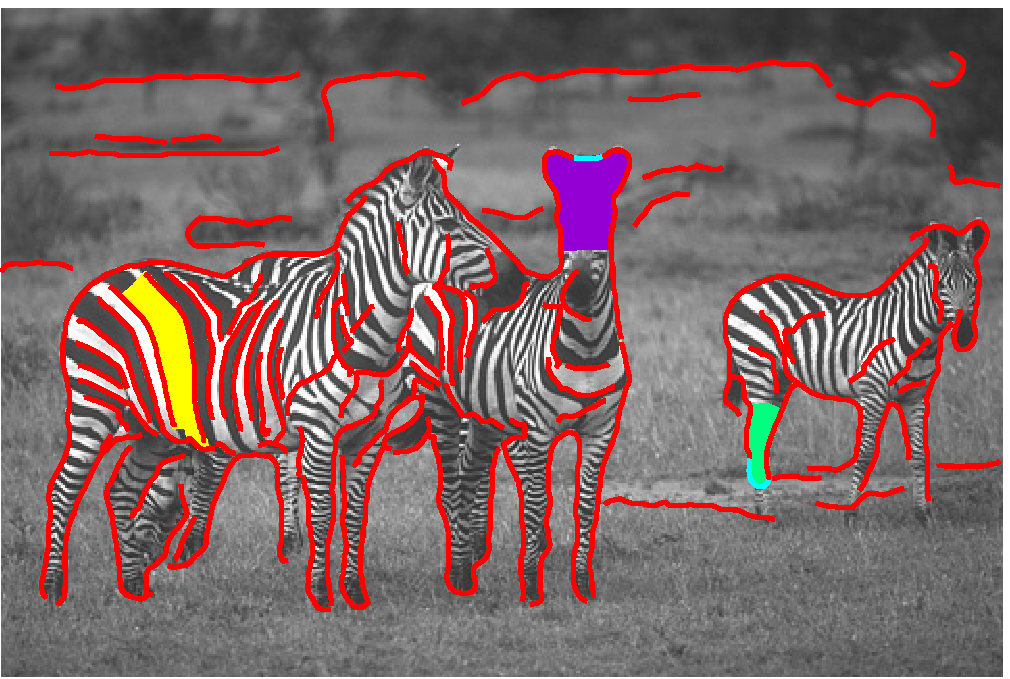
\includegraphics[width=0.32\linewidth]{figs/zebra_t1.pdf} &
{\footnotesize\textit{i}} 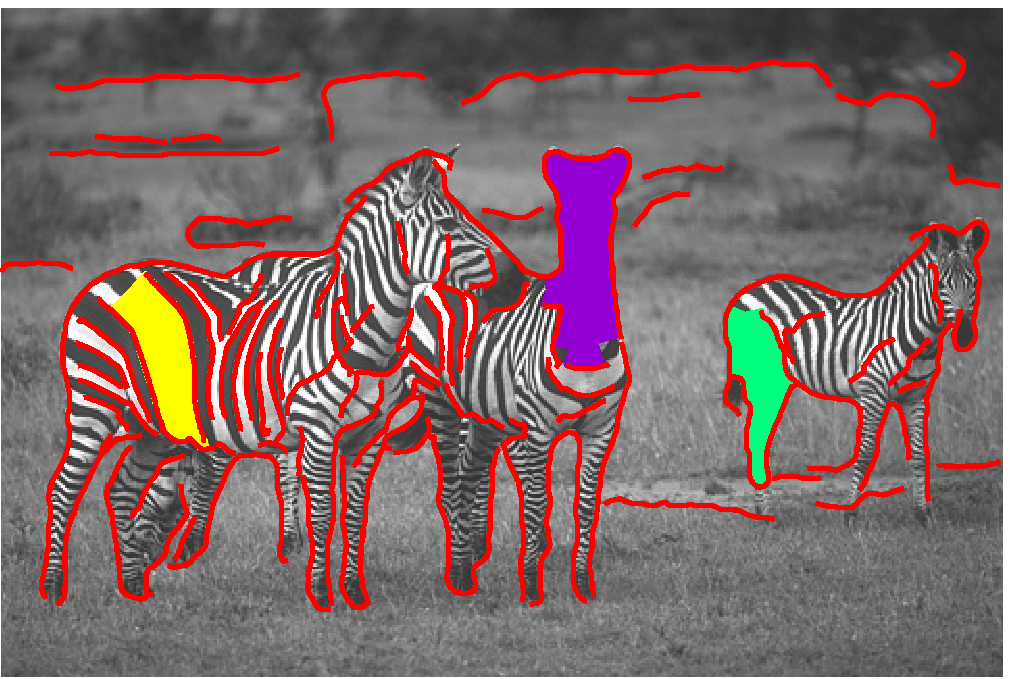
\includegraphics[width=0.32\linewidth]{figs/zebra_t2.pdf}
\end{tabular}
{\footnotesize\textit{j}} 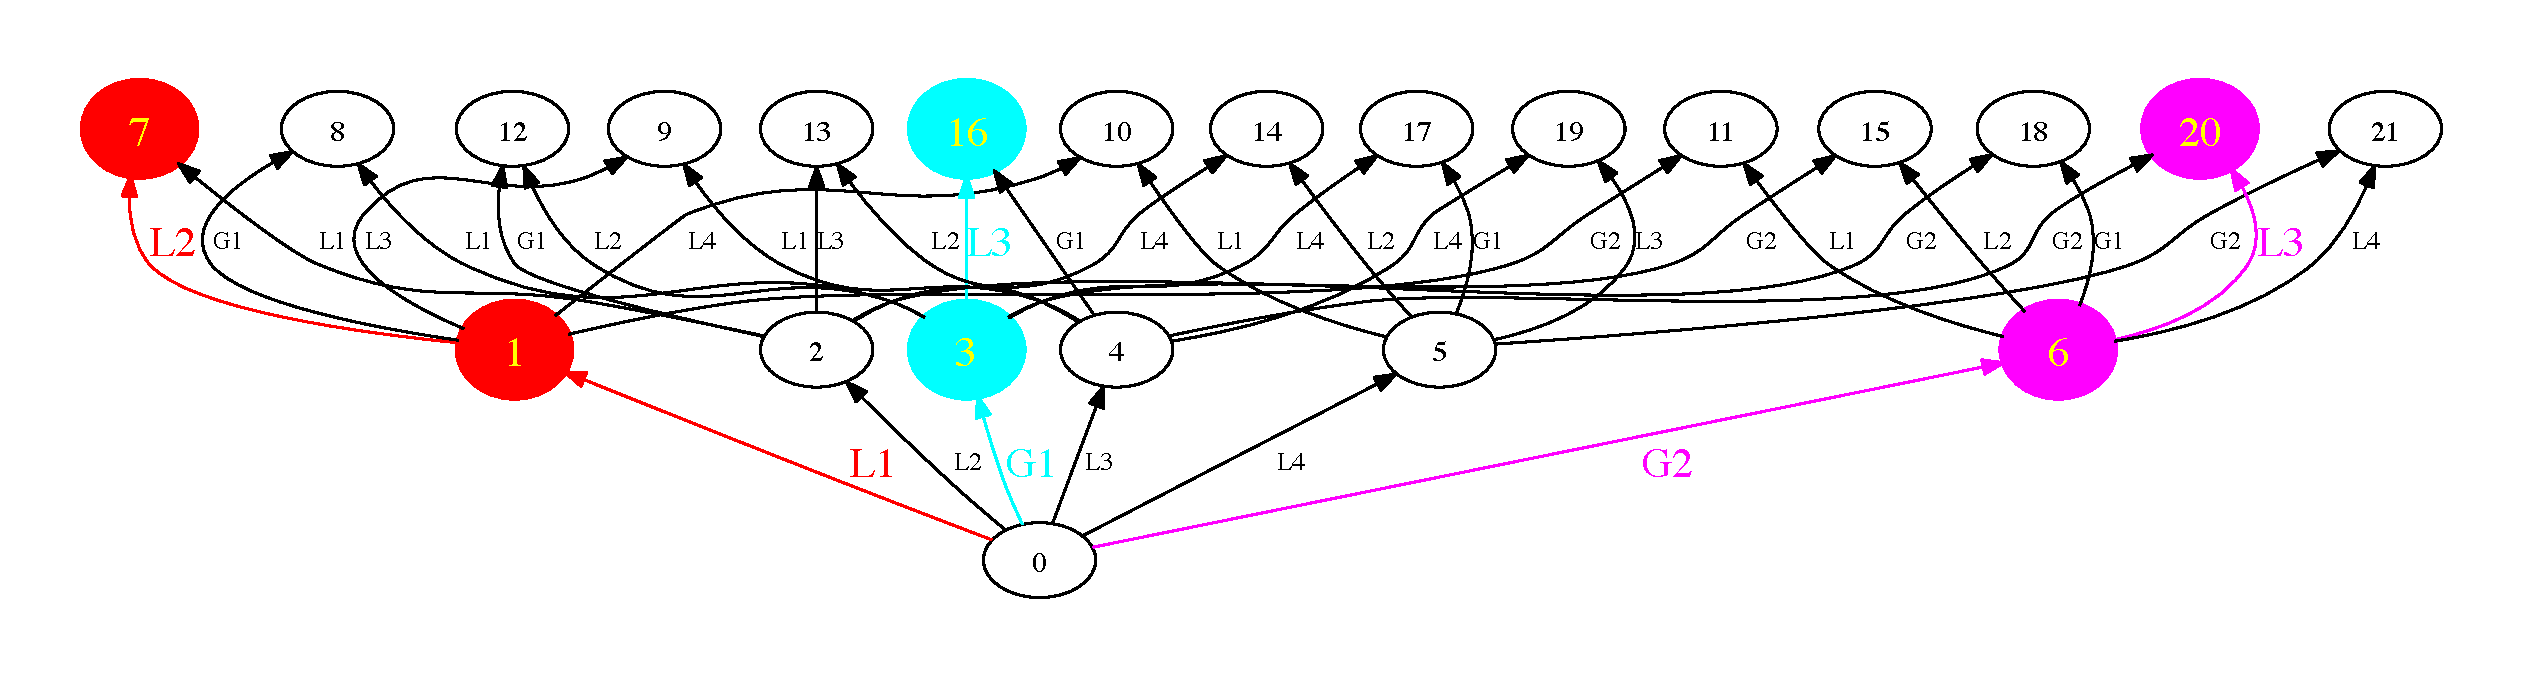
\includegraphics[width=0.645\linewidth]{figs/zebra_full_cgraph.pdf}
{\footnotesize\textit{k}} 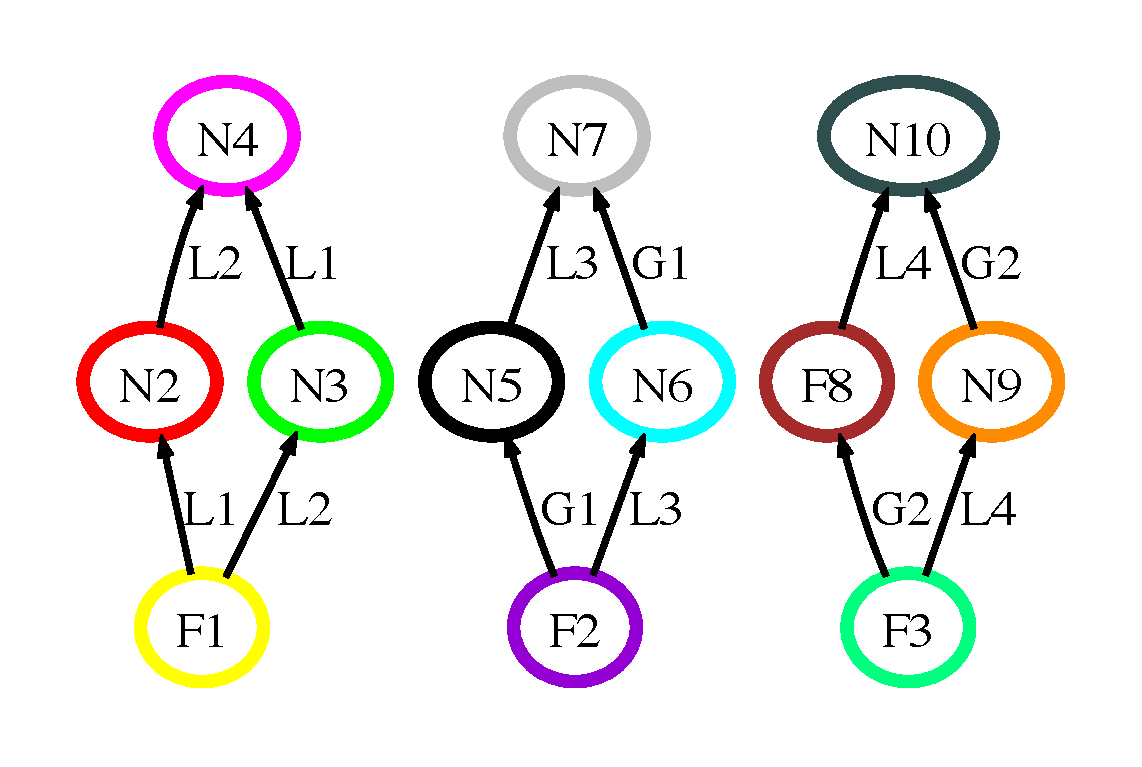
\includegraphics[width=0.32\linewidth]{figs/cgraph_zebra_frags.pdf}
\caption{Reduction of search space through clustering transforms. a) The spatial distribution of transforms each indicated by a blue dot. b) Clustering based on dividing up the image and considering sets of transforms in each square. c) Another approach to clustering based on sampling a set of transforms and using the Voronoi Diagram to divide up the image region into clusters of transforms. d) The initial set of seed MVFs and the (e) fragment centric assignment of transforms to seeds; each transform's color corresponds to a seed fragment. (transforms are typically applicable to multiple fragments so one color was randomly selected for each transform). (f) A selection of three seed MVFs $F_1$,$F_2$, and $F_3$ for the purpose of illustration and the transforms applicable to each fragment are shown in (g). (h) Application of transforms $(L_1)$,$(G_1)$, and $(G_2)$ to $F_1$,$F_2$, and $F_3$, respectively. (i) The application of transforms $(L_1,L_2)$, $(G_1,L_3)$, and $(G_2,L_4)$ to $F_1$,$F_2$, and $F_3$ respectively. Observe how the two-length transform sequence search space reduces from (j) to (k) by adopting a fragment-centric approach. The savings are much more dramatic when a large number of transforms appear in a sequence. There are typically 50-100 seed MVFs chosen for each image.}
 \label{fig:cluster}
%\vspace{-0.751cm}
 \end{figure*}


An explicit clustering of transforms requires a computation of pairwise dependency between transforms, \ie, capturing the graph of red links connecting blue nodes in Figure~\ref{fig:indep}\textcolor{red}{e,f} which is computationally expensive. However, observe that spatially segregated transforms are typically independent. Thus, the space of transforms can be {\em implicitly clustered} spatially by partitioning the image into areas where transforms in each area are identified as belonging together. Each set of transforms would thus have some limited interaction with the neighboring sets, see Figure~\ref{fig:cluster}\textcolor{red}{b}. Alternatively we could use a subsampling of the locations of the transforms and divide up the image using a Voronoi diagram to partition the transforms into sets, Figure~\ref{fig:cluster}\textcolor{red}{c}, belonging to each Voronoi cell. 


The clustering of transforms reduces the search space significantly, but it is unfortunately still too large for a practical search. The main reason is that the indiscriminate exploration of transform sequences with each cluster is unguided by a sense of object part formation. Additional savings can be earned when the sequence of transforms is encouraged to form objects by grouping and modifying a select seed MVF fragment. The seed fragments, Figure~\ref{fig:cluster}\textcolor{red}{(d)}, are chosen to have a high likelihood of being part of an object, \ie, be of Type I, have a veridical contour ( at least 40\% ), be fairly homogenous inside, \etc. The seed is then transformed by any of the transforms applicable to it, and the process is repeated. This restricts the transform sequences to be concerned with the formation of an object part by modifying select seeds, thus discarding those not concerned with it. For example, if a set of transform sequences contains $\{T_1,T_2,T_3,T_4\}$ and the seed MVF is connected with $T_3$, then the transforms that are considered are $\{(T_3),(T_3T_1),(T_3T_2),(T_3T_4),(T_3T_1T_2),(T_3T_1T_4),(T_3T_2T_1),(T_3T_2T_4),(T_3T_4T_1),(T_3T_4T_2),\newline(T_3T_1T_2T_4)(T_3T_1T_4T_2),(T_3T_2T_1T_4),(T_3T_2T_4T_1),(T_3T_4T_1T_2), and (T_3T_4T_2T_1)\}$, 16 in total, \ie, ($\frac{3!}{3!}+\frac{3!}{2!}+\frac{3!}{1!}+\frac{3!}{0!}=1+3+6+6=16)$, but all sequences starting with $T_1,T_2,T_4$ are not explicitly considered, namely the 48 (3x16) sequences starting with $T_1$, $T_2$, or $T_4$. Due to a significant level of order independence, however, those transforms which begin with $T_1$, $T_2$, or $T_4$ but also contain $T_3$ are already covered, that is 33 (3x11) of 48 transforms so that only 15 (48-33) transforms are completely discarded, namely, $\{(T_1),(T_2),(T_4),(T_1T_2),(T_1,T_4),(T_2,T_1),(T_2,T_4),(T_4T_1),(T_4T_2),\newline(T_1T_2T_4),(T_1T_4T_2),(T_2T_1T_4),(T_2T_4T_1),(T_4T_1T_2),(T_4T_2T_1)\}$, which counts as $\frac{3!}{2!}+\frac{3!}{1!}+\frac{3!}{0!}=3+6+6=15$ transforms. Some of these 15 discarded transform sequences are equivalent due to order independence so the effective number of discarded transforms reduces to $\frac{3!}{2!1!}+\frac{3!}{1!2!}+\frac{3!}{0!3!}=3+3+1=7$. In general with a set involving $N!$, insisting on sequences that begin with one particular transform and assuming order independence discards only $\sum_{i=k}^{N-1}\binom{N-1}{k!}=(2^{N-1}-1)$ transforms, Figure~\ref{fig:trans_missed}. Figure~\ref{fig:cluster}\textcolor{red}{(e)} identifies the cluster of transforms formed by each seed, Figure~\ref{fig:cluster}\textcolor{red}{(d)}, by assigning a random color. In general, our seeding generates clusters about four to five transforms so that the number of discarded transforms is on the order of five to six per image. 

%% Considering that \emph{(i)} most organization of pixels into objects involve multiple transform sequences and that \emph{(ii)} these sequences are often order independent, we can make a further simplification by considering only the set of transform sequences that begin with the transforms at sample seed locations. This is effectively a focused effort to begin with some MVFs and modify it toward objects or object parts. In this fragment centric approach, transforms that operate on other MVF neighboring fragments can only be considered when they appear as apart of another transform sequence that involves the seed transform so essentially single or pairs of transforms not close to the seeds are discarded. We compensate for this by selecting seed transforms judiciously. Seed MVFs, Figure~\ref{fig:cluster}\textcolor{red}{(d)}, are those which are Type 1, and that further have a sufficient level of real contour versus virtual contour (at least 40\% percent) so that the seed MVFs are likely to be part of the objects in the scene. The number of seed fragments are typically on the order of 50 to 100. Figure~\ref{fig:cluster}\textcolor{red}{(e)} identifies the clusters of transforms created by each respective seed fragment by uniquely coloring them. 



%% \caption{a) An image with various transforms initially detected indicated as blue dots. b) Clustering based on dividing up the image and considering sets of transforms in each box. c) Another approach to clustering based on sampling a set of transforms and using the Voronoi Triangulation. d) The initial set of seed MVFs and the (e) clustering of transforms given these seeds. Each set of transforms is uniquely colored to represent the transforms indexed by that individual seed.  f) Three seed fragments $F_1,F_2,$ and $F_3$ and (g) their zoomed in location with an initial set of detected transforms. h) We observe one length sequences $F_1 \rightarrow L_1,F_2 \rightarrow G_1,F_3 \rightarrow G_2$ and two length sequences (i) $F_1 \rightarrow L_1L_2,F_2 \rightarrow G_1L_3,F_3 \rightarrow G_2L_4$ from each of these seed fragments. j) The search space if we assume no clustering based on MVF. The various sequences are highlighted as the red, cyan, and magenta paths in the graph. j) The search space if we do take advantage of seed MVFs. Various two-length sequences can be formed by collating the results from these three independent sets. }

%% Restricting transforms to initiate at seed MVFs discards certain transform sequences. 



\begin{figure}[ht]
\centering
  {\footnotesize\textit{\textcolor{black}{a)}}}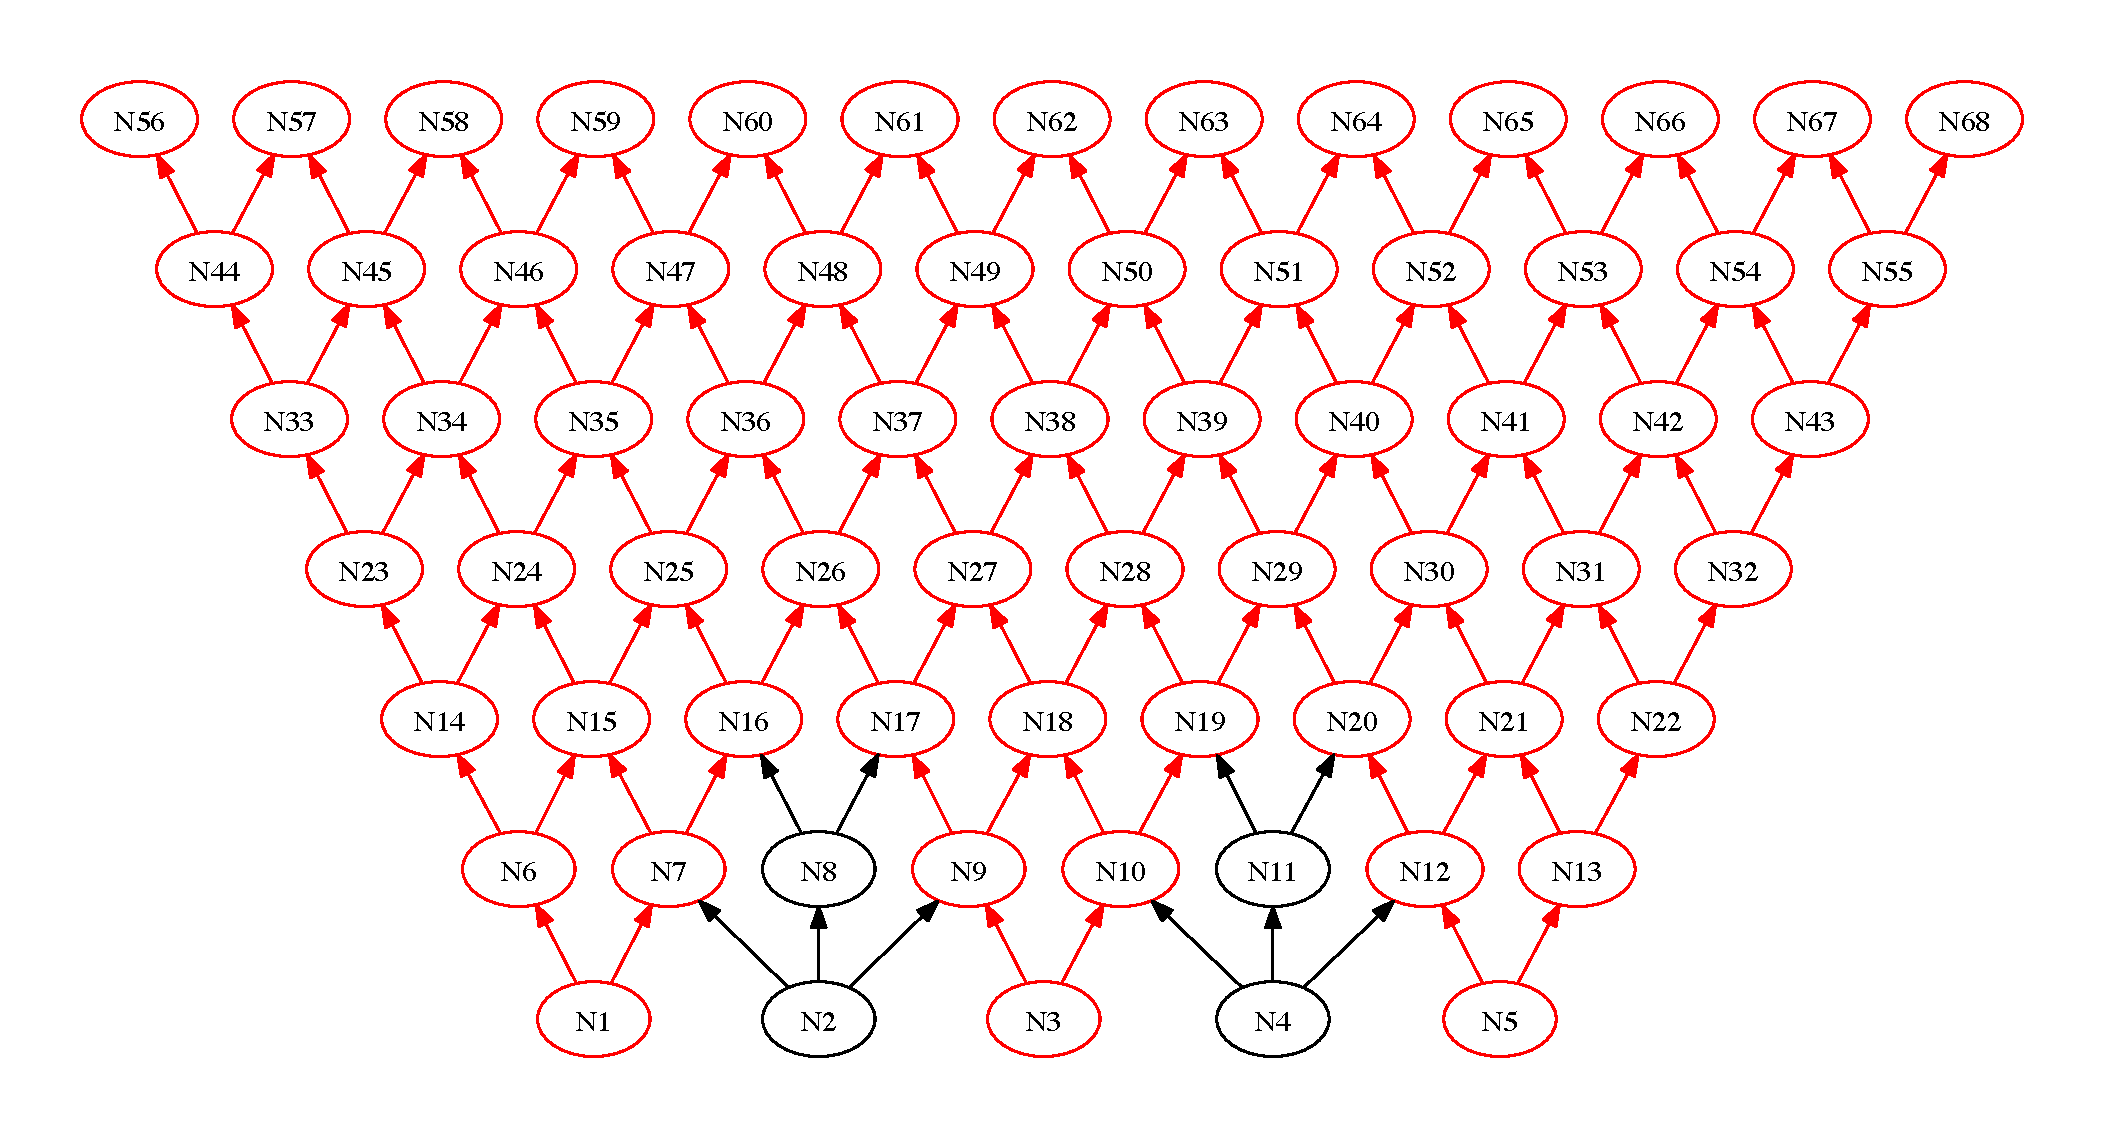
\includegraphics[width=0.3\textwidth]{figs/spacing_small.pdf} 
  {\footnotesize\textit{\textcolor{black}{b)}}}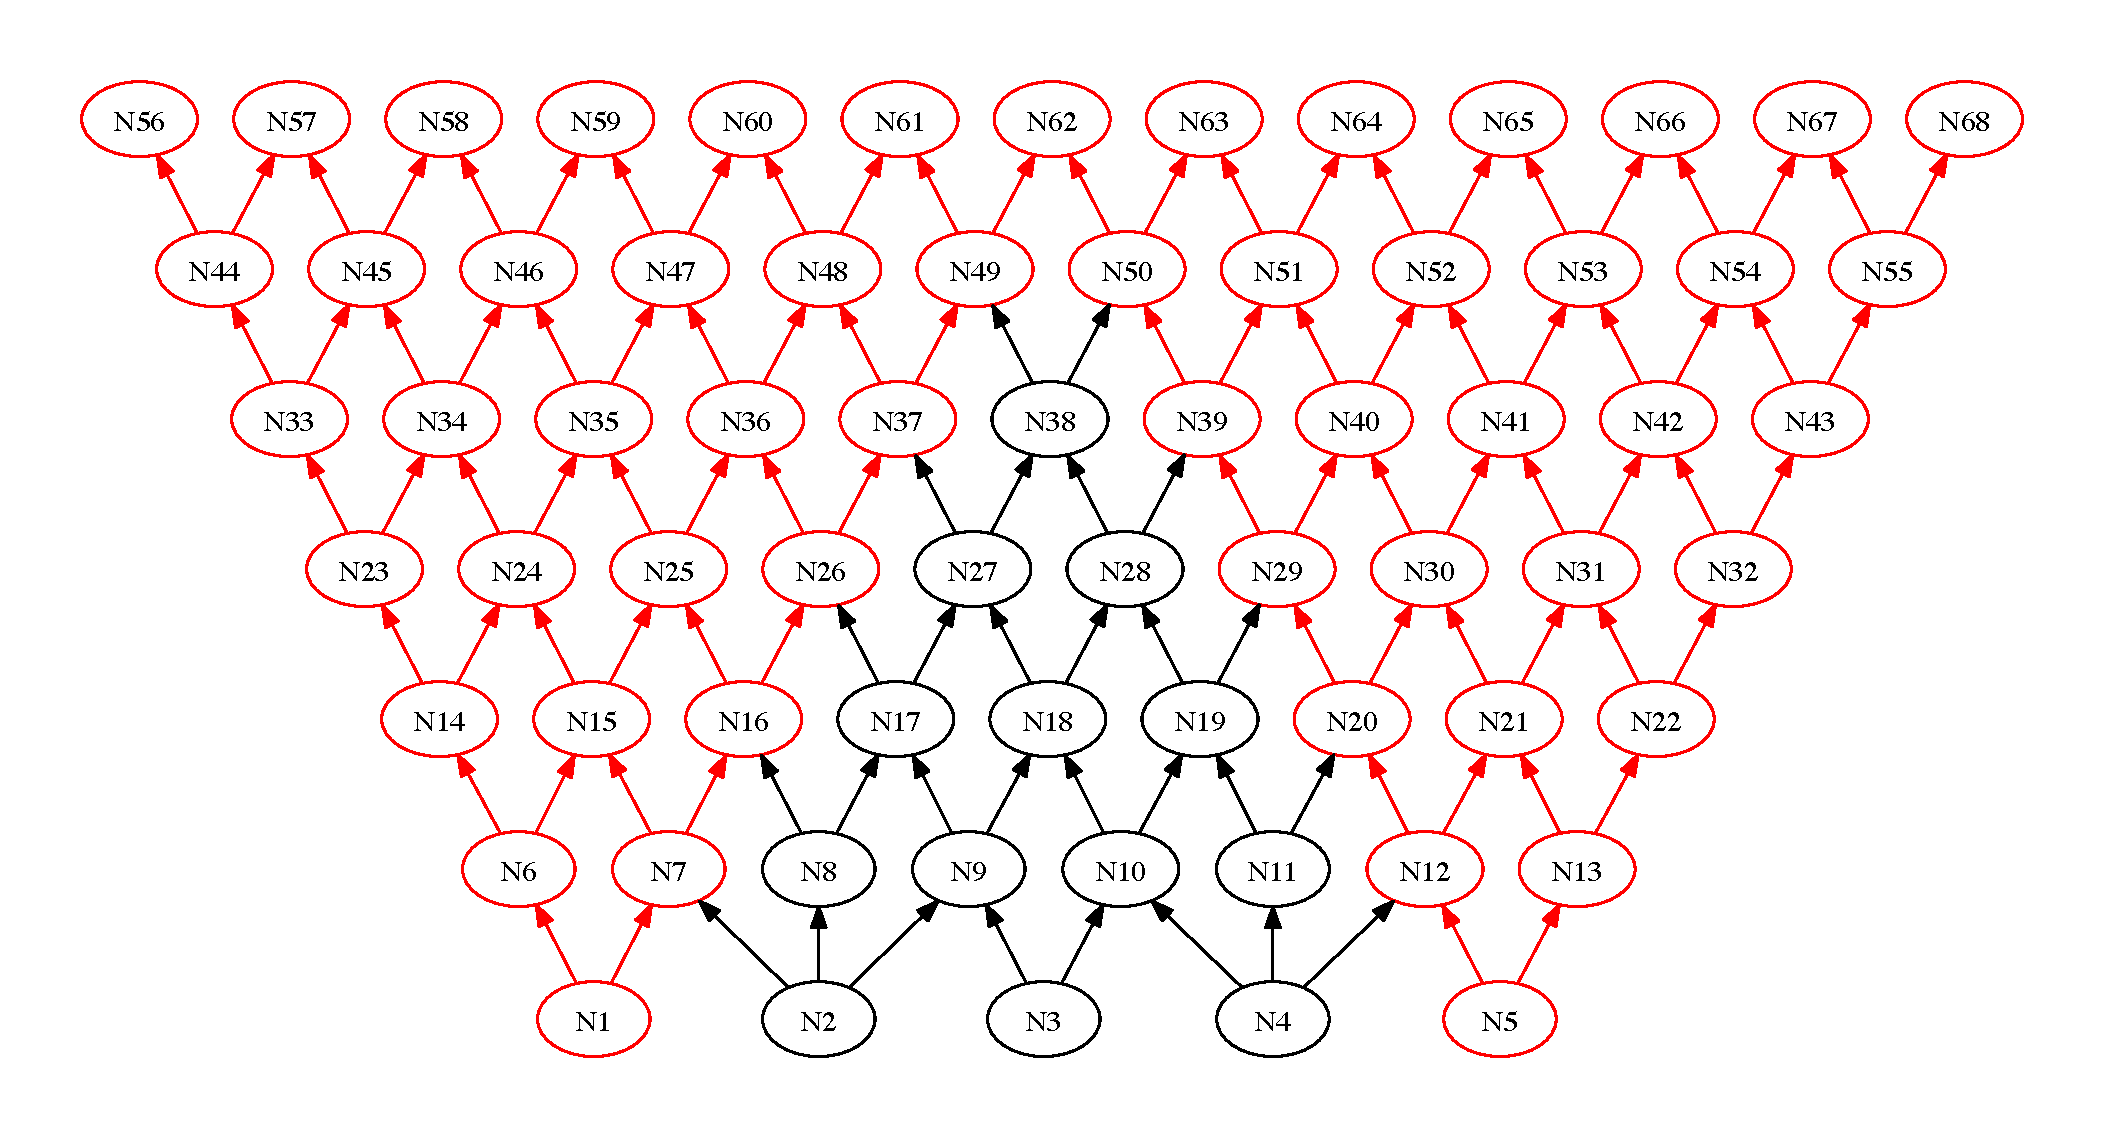
\includegraphics[width=0.3\textwidth]{figs/spacing_large.pdf} 
\caption{a) An illustration of transform sequences that are discarded as a result of considering transform sequences from select MVF seeds. All transform sequences in black are discarded. b) If samples are not uniformly distributed, there is an exponential increase in the number of unexplored/discarded transform sequences. }
\label{fig:trans_missed} 
\end{figure}


 %% \textcolor{red}{To Ben: there is no fancy seed strategy , I essentially expand from ONLY type-1 MVS , i only have one requirement that the seeds have enough real contour versus virtual ... a better way of asking this is do we have some seed strategy ? ...my strategy (cant even call it that)  is very dumb, there is so much overlap in terms of transforms indexed}  



%% Consider now a single dependency is introduced between these two independent sets $T$ and $\overline{T}$, Figure~\ref{fig:cluster_sets}\textcolor{red}{b}. Any transform sequence that does not contain both $T_3$ and $T_2$ can essentially be considered as two independent subsequences, as before. Transform sequences that contain both $T_3$ and $T_2$ are either invalid, thus leading to a slight modification in the overall search space, or if the presence of the $T_3$ affects $T_2$ results, then the sequence containing both cannot be considered independently.  

%% The significant reduction of the search space as a result of grouping transforms into roughly independent set of transforms can be done though a clustering of transforms. However, the determination of pairwise dependency, \ie,




Figure~\ref{fig:cluster} illustrates the idea of exploring the search space by expanding from a set of seed medial visual fragments, namely seeds $F_1$,$F_2$, and $F_3$, Figure~\ref{fig:cluster}\textcolor{red}{(f)}. Each seed initially detects, Figure~\ref{fig:cluster}\textcolor{red}{(g)}, two possible transforms. Figures~\ref{fig:cluster}\textcolor{red}{(h,i)} show how each seed fragment evolves by applying one and two length transform sequences respectively: Fragment $F_1$ explores the sequence $(L_1)$ then $(L_1,L_2)$ and $F_3$ explores transform $(G_2)$ followed by sequence $(G_2,L_4)$. The search space representing these particular sequences among all possible one and two length sequences is represented in Figure~\ref{fig:cluster}\textcolor{red}{(j)}. Observe however that $F_1$,$F_2$, and $F_3$ form independent sets of length two transforms implying that the search space in Figure~\ref{fig:cluster}\textcolor{red}{(k)} can be used to interleave transforms to achieve Figure~\ref{fig:cluster}\textcolor{red}{(j)} implicitly. While not depicted, the savings is even greater if we consider all possible sequences since the full search space consists of 63 ($2^6-1$) nodes, while all $K$ length sequences could be equivalently recovered by just exploring directed paths in Figure~\ref{fig:cluster}\textcolor{red}{(k)} and interleaving them. 

The computational savings in this particular case and in general can be quantified by Equation~\ref{eq:complexity3} if the seeding strategy leads to $M$ independent sets. The savings will continue to increase as the number of seed MVFs increases, Figure~\ref{fig:frag_growth_redun}. Realistically, though, as we continue to increase the number of seeds the reduction in the size of the search space saturates. For example, in Figure~\ref{fig:cluster}\textcolor{red}{(d)} we observe seed MVFs directly adjacent to each other due to the zebra stripe pattern. Exploration from any one of these seeds will cover all transform sequences within that area. Visiting the rest of the zebra stripe seeds does not reduce the search space any further, but rather wastes computational resources revisiting previously searched transformed sequences. This wasted effort is severely mitigated by the fact that seeds attempting to explore previously visited sequences will be terminated as the system tracks all previously explored states (nodes in the graph).   

%% \begin{figure}[ht]
%% \centering
%% 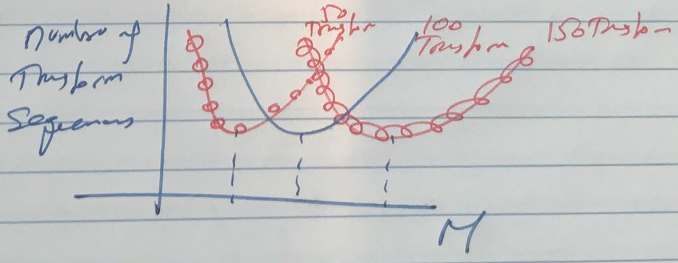
\includegraphics[width=0.25\textwidth]{figs/savings_seeds.png}
%% \caption{The reduction in the number of transform sequences grows till a point as we increase the number of seeds. After some point we achieve no further benefits of increasing the number of seeds, but instead incur a small computational hit. }
%% \label{fig:seed_savings}
%% \end{figure}

 %% If all seeds for a given image lead to independent sets of transforms then our savings would be exactly captured by Equation~\ref{eq:complexity3}. In general, however, 


%% for  which would lead to to a much larger tree, Fig



%% In this particular example, given that all three sets are independent 



%% consider we look at how the underlying structure of the space changes. In the previous examples, Figures~\ref{fig:seq_cgraphs}\textcolor{red}{(a,b)} the search space was explored without any partitioning \ie exploring all transforms globally. If we apply the same global scheme to Figure~\ref{fig:cluster}\textcolor{red}{a} we would end up the graph shown in Figure~\ref{fig:cluster}\textcolor{red}{i}. We don't show the full graph as for six transforms we would have to consider sixty three transform sequences. If however, we explore the space of all transform sequences restricted to to the case of selecting only three seed fragments, $F_1$, $F_2$, and $F_3$, shown in yellow, purple and green respectively, and each zoomed in Figure~\ref{fig:cluster}\textcolor{red}{f}. Figure~\ref{fig:cluster}\textcolor{red}{g} and Figure~\ref{fig:cluster}\textcolor{red}{h} show transform sequences of length one and two respectively applied to each fragment. Figure~\ref{fig:cluster}\textcolor{red}{i} shows those transforms as part of the overall transform possibilities applied to the image and Figure~\ref{fig:cluster}\textcolor{red}{j} shows possible transforms restricted to fragments $F_1$,$F_2$, and $F_3$. In general, if $M$ seed transforms from $N$ transforms are chosen and assuming that transforms are equally distributed to as set of $\floor*{\frac{N}{M}}$ transforms each, and if these sets are {\bf independent} thus the total number of nodes is 


 %% our representation changes to Figure~\ref{fig:cluster}\textcolor{red}{j}. Comparing Figure~\ref{fig:cluster}\textcolor{red}{m} and Figure~\ref{fig:cluster}\textcolor{red}{n} we see that in a global expansion we explore the cross product combination of all these transforms leading to length three, four, five, and six sequences which are discarded in the local version. We have drastically reduced the number of transforms we need to consider from sixty three to nine! These savings can be quantified by changing our equations to reflect a local search algorithm versus a global one. If we start from $M$ medial visual fragment and assume each fragment indexes the same number of transforms, $N$, then our new complexity is Equation~\ref{eq:complexity3}, where $\floor*{\frac{N}{M}}$ represents the number of transforms explored by each of the $M$ medial visual fragments.

%% It is important to note that this assumption of {\bf independent} and {\bf equal} sets of transforms is not realistic. Observe that in Figure~\ref{fig:cluster}\textcolor{red}{d} we see a sampling of various Type 1 Medial Visual Fragments that could possibly serve as seed fragments. The transforms indexed by each Type 1 MVF is indicated as a polygon with blue dots lying within the polygon representing reachable transforms. More over many polygons overlap which indicates Type 1 Medial Visual Fragments are indexing the same sets of transforms. It is difficult to model dependent/non-equal/overlapping sets of transforms so we model each set as independent, analogous to the synthetic example in Figure~\ref{fig:indep}\textcolor{red}{a}, to arrive at Equation~\ref{eq:complexity3}. 



%% We begin our analysis by understanding the search space of the previous examples in Section~\ref{sec:transform_seq}. Revisiting Figure~\ref{fig:snake_seq}, three transforms exist, and if we utilize Equation~\ref{eq:complexity} it states that our search space is composed of fifteen transform sequences. How can we model all these possibilities? We can capture all these transform sequences as a search tree, Figure~\ref{fig:seq_cgraphs}\textcolor{red}{a}. In this view, nodes of the tree capture, our RECOIN representation, and edge each of the tree represents an applicable transform ( insertion of contour, removal of contour, etc). Each directed path within the tree maps to one of the fifteen possible transform sequences. The two sequences explored in Figure~\ref{fig:snake_seq}, marked as cyan and red paths in Figure~\ref{fig:seq_cgraphs}\textcolor{red}{a}, represent a small exploration of the total number of paths to consider. Again, it is important to realize that Equation~\ref{eq:complexity} does \emph{not} specify which paths or how many to explore, but only bounds the \emph{number} of paths to consider. Finally, the structure of this search tree, is conceptually similar to the AND/OR tree representation utilized in computer science. At each node of the tree we can either explore this \emph{or} that transform, and paths in the tree represent applying this transform \emph{and} that transform. However, compared to its original goal, which was recently utilized in~\cite{Si:Zhu:PAMI13}, to model precedence relationships \ie this state can only occur if this \emph{and} this happen \emph{or} that occurs, our tree-structure is not defined by such relationships. 




  

%% We see the sequence outlined in Figure~\ref{fig:snake_seq} represented as the \textcolor{red}{red path} in the containment graph. Nodes $N_1$,$N_2$,and $N_4$ correspond to Figures~\ref{fig:snake_seq}\textcolor{red}{a,b,c} and \textcolor{red}{d} respectively.  

%% The two alternative sequences outlined in Figure~\ref{fig:mushroom_seq_a} and Figure~\ref{fig:mushroom_seq_b} can be effectively captured by one graph. Node $N_2$ corresponds to taking the path captured in Figure~\ref{fig:mushroom_seq_a} and the alternative path $N_1\rightarrow N_3\rightarrow N_5 \rightarrow N_6$ is captured by subfigures Figure~\ref{fig:mushroom_seq_b}\textcolor{red}{a,b,c} and \textcolor{red}{d} respectively.

%% The tree structure for this simple example highlights that even with a minimal number of transforms (3) there are a wide array of possible transform sequences or paths to consider. However, much of the search space is composed of duplicate sequences. As we analyzed earlier in Figure~\ref{fig:snake_seq} the transform sequence $G_1 \rightarrow L_1 \rightarrow G_2$ duplicates the work of $G_2 \rightarrow G_1 \rightarrow L_1$ as both lead to the same final transformed state. Rather than explore both of these sequences, highlighted as \textcolor{red}{red} and \textcolor{cyan}{cyan} respectively in Figure~\ref{fig:seq_cgraphs}\textcolor{red}{a}, we can arrive at the same state by just exploring one. Another example of this duplication is the path $N_1 \xrightarrow[]{G_1} N_2 \xrightarrow[]{L_1} N_6$ which leads to a final representation identical to the one if we had taken the path $N_1 \xrightarrow[]{L_1} N_3 \xrightarrow[]{G_1} N_7$ instead. Any ordering of these transforms, or edges of the tree, lead to the same final state, i.e. $N_6 == N_7$. This duplication or redundancy in transform sequences can effectively be pruned from our search space without losing anything. How can we capture these redundancies in the search space? Rather than let each path in our tree grow independent of others we ask does the path I am considering lead to the same representation as any other path, and if so merge the equivalent paths to a single node. The dramatic effect of this can be seen in Figure~\ref{fig:seq_cgraphs}\textcolor{red}{b}. We observe a huge reduction in the total number of nodes to explore, from sixteen to eight, but even more importantly our representation has shifted from a tree to a graph due to the presence of these directed cycles capturing equivalent transform sequences. The effect on the complexity of our space is just as dramatic as now the growth of Equation~\ref{eq:complexity} has been severely curtailed, Equation~\ref{eq:complexity2}. 


%% If we compare the growth of our space, Figure~\ref{fig:ss_growth_redun}, with this reduction we notice that we have reduced the growth rate by a factorial. Utilizing Equation~\ref{eq:complexity2} for this current example, the space of transform sequences shrinks to just seven sequences, $\{(G_1),(G_2),(L_1)(G_1,G_2),(G_1,L_1),(G_2,L_1)(G_1,G_2,L_1)\}$, from the original fifteen. Again, this does not mean that our new graph structure has only seven paths mapping to each of the seven transform sequences, but rather the total number of distinct paths is bounded by this number. If we look at Figure~\ref{fig:seq_cgraphs}\textcolor{red}{b} the graph structure has twelve different paths, which on the surface does not seem that big of a reduction compared to the fifteen paths in the original tree structure. However, the key insight is that by capturing redundancies the computational savings is \emph{not} the reduced set of transform sequences we explore but rather the huge set of transform sequences that we \emph{do not} explore. Assume we take the paths $N_1 \xrightarrow[]{G_1} N_2 \xrightarrow[]{G_2} N_5$ and  $N_1 \xrightarrow[]{G_2} N_4 \xrightarrow[]{G_1} N_9$ in Figure~\ref{fig:seq_cgraphs}\textcolor{red}{a}. Both of these paths lead to the same transformed state, $N_5$ and $N_9$, and even more they lead to identical children nodes and subtrees. By treating them as independent paths, we end up doing twice as much exploration. However, in the graph formulation, these two paths, merge into Node $N_5$ so even if we were to mistakenly explore these two redundant sequences or any pair of redundant sequences for that matter, we ensure that any future exploration of transform sequences, out edges of the node, only happen once.

%% 

\noindent\\
{\bf III Reduction through Transform Dynamics: } The set of applicable transforms is not static: the application of a transform can nullify the application of another transform or it can introduce a new one. In a previous example, Figure~\ref{fig:snake_seq}, all transforms were applied to our representation without affecting the detection/application of the other transforms and in addition no new transforms were introduced. In contrast, Figure~\ref{fig:mushroom_seq} depicts the more realistic situation of a set of transforms which are inter-dependent, \ie, the application of a transform renders some transforms inapplicable and also introduces new transforms. In practice, the number of candidate transforms that are disqualified as a result of a recently applied transform is overwhelmingly more than the number of newly introduced transforms: examining over hundreds of images we computed that on average the application of a transform is connected to $2.30\pm1.64$ dependent neighbors, Figure~\ref{fig:indep}\textcolor{red}{(e,f)}. 

\begin{figure}[ht]
  \centering
%% {\footnotesize\textit{\textcolor{black}{a)}}}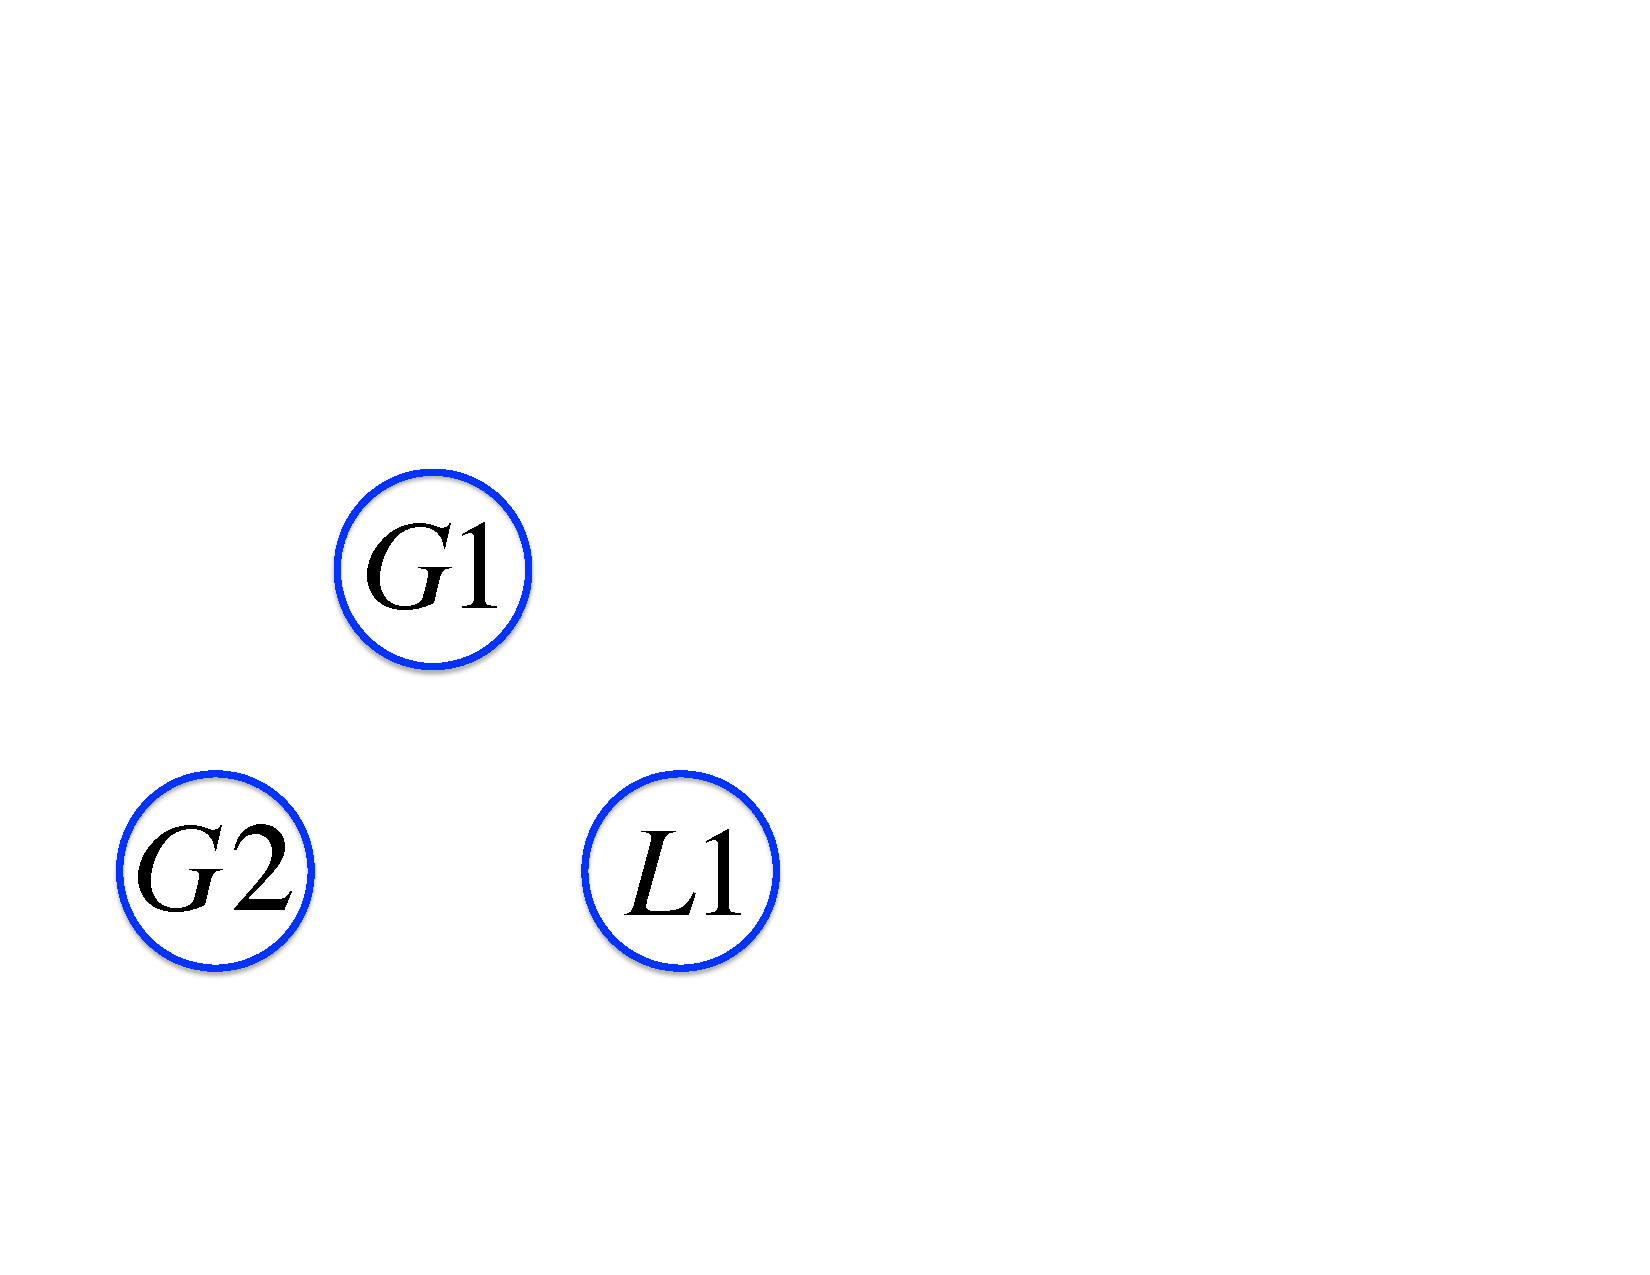
\includegraphics[width=0.15\textwidth]{figs/snake_depend.pdf} 
%% {\footnotesize\textit{\textcolor{black}{b)}}}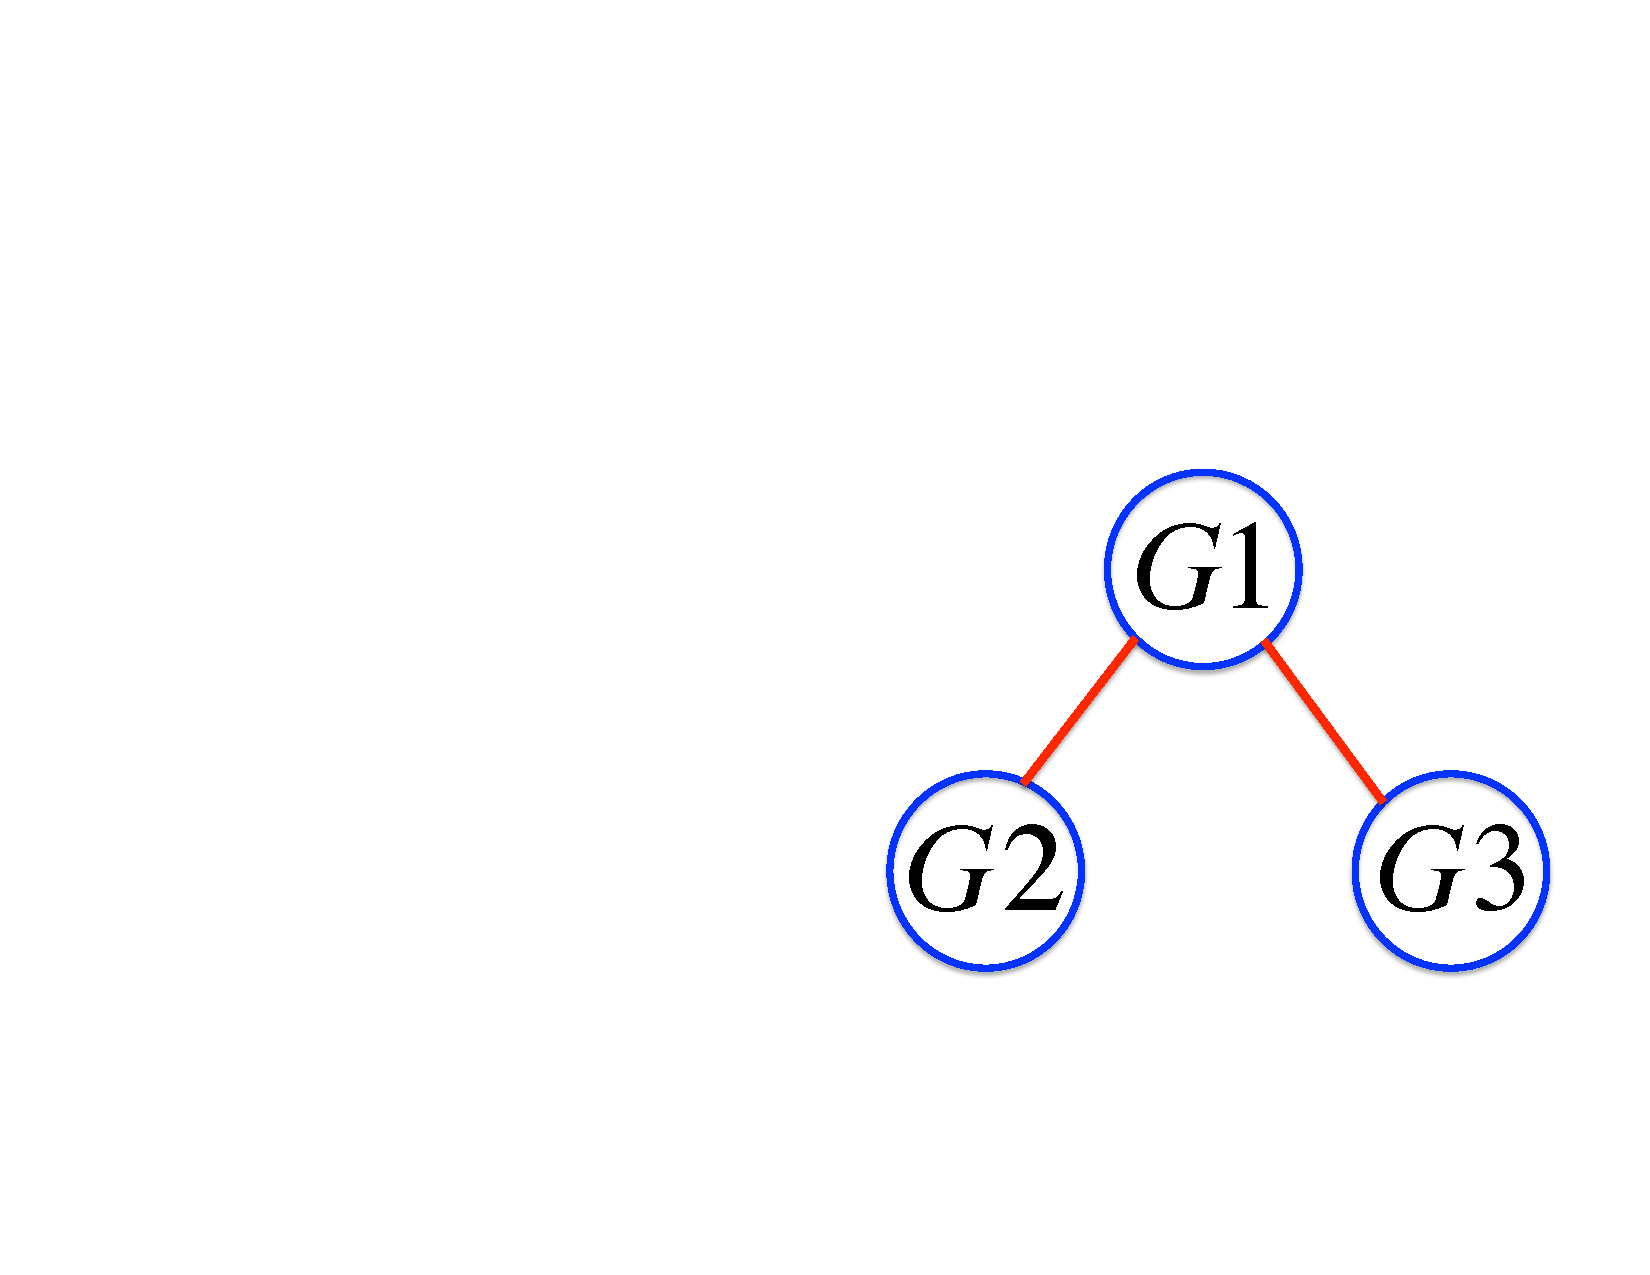
\includegraphics[width=0.15\textwidth]{figs/mushroom_depend.pdf} 
  {\footnotesize\textit{\textcolor{black}{a)}}}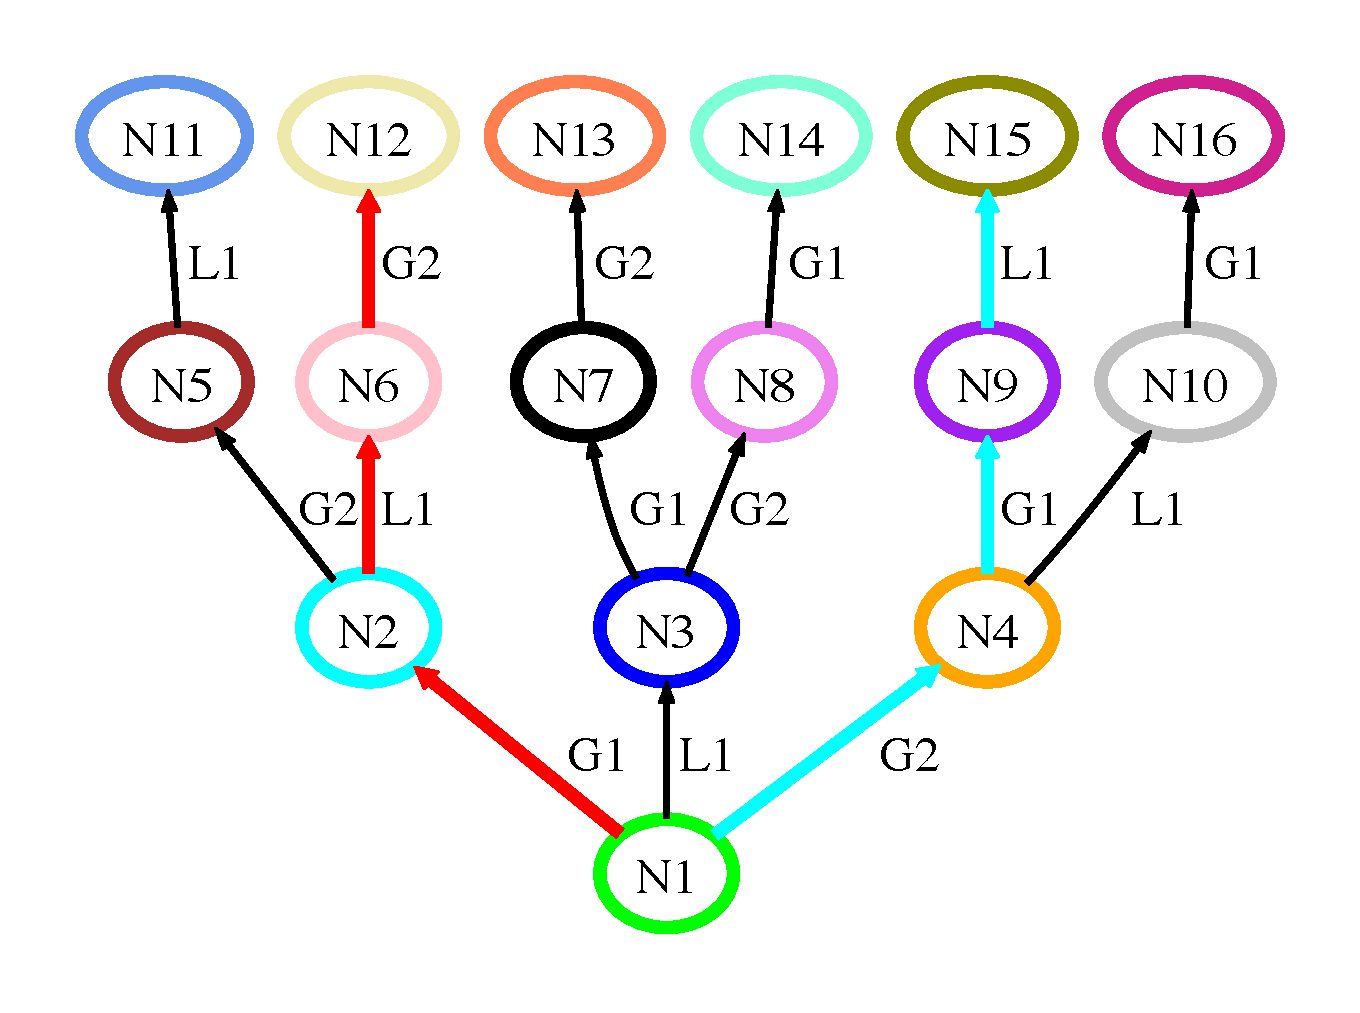
\includegraphics[height=0.22\textwidth]{figs/full_snake_cgraph_no_red.pdf} 
  {\footnotesize\textit{\textcolor{black}{b)}}}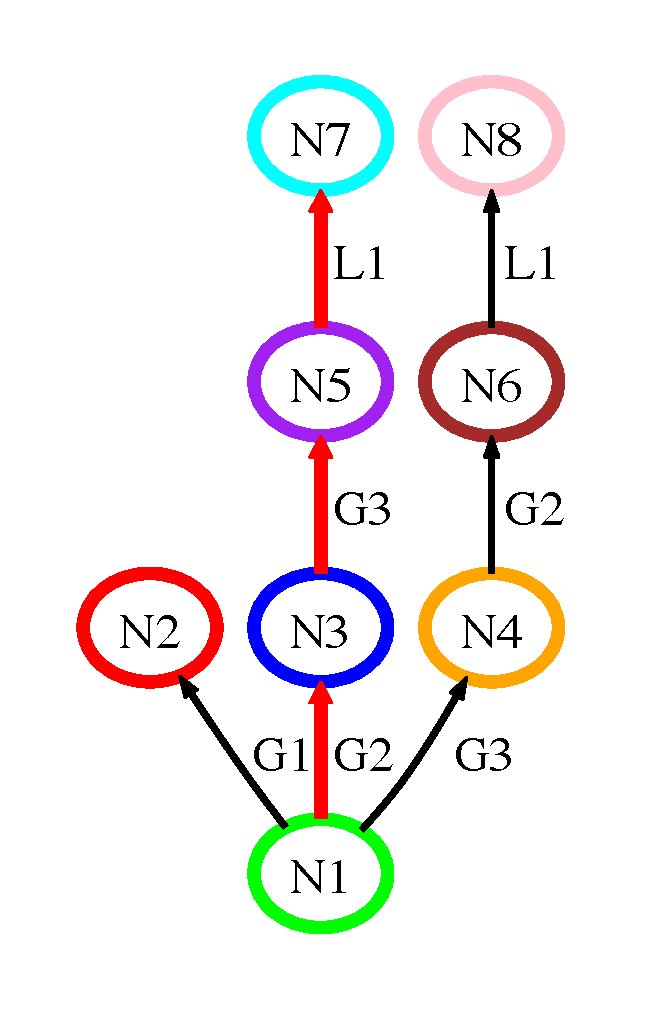
\includegraphics[height=0.22\textwidth]{figs/full_mushroom_cgraph_no_red.pdf} 
  {\footnotesize\textit{\textcolor{black}{c)}}}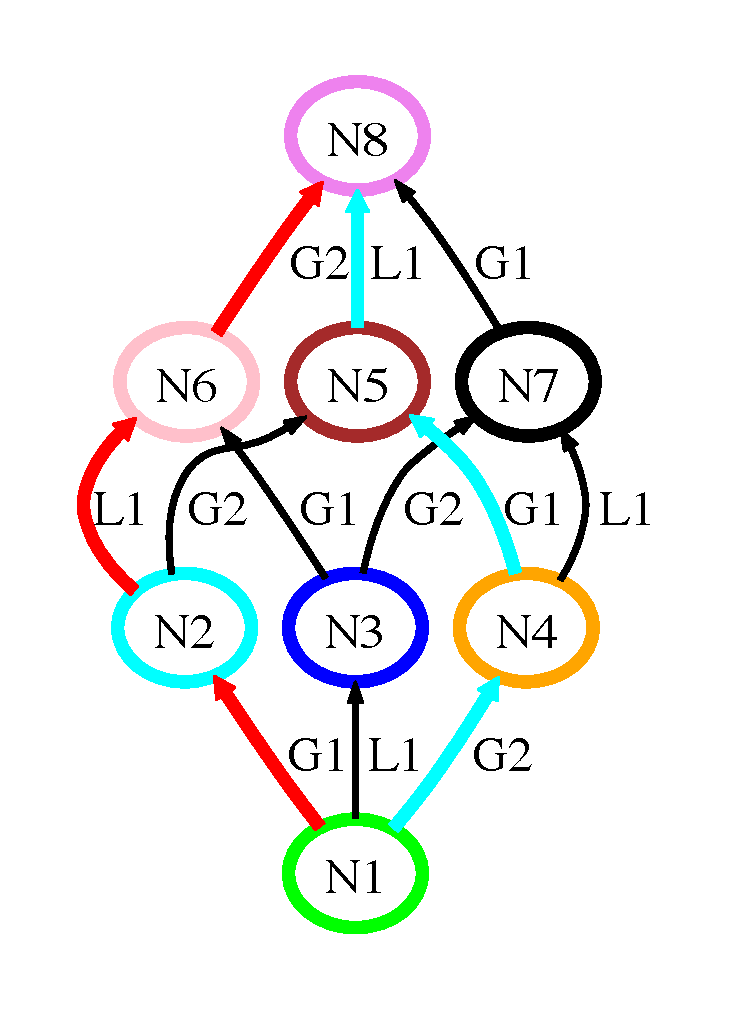
\includegraphics[height=0.22\textwidth]{figs/full_snake_cgraph.pdf} 
  {\footnotesize\textit{\textcolor{black}{d)}}}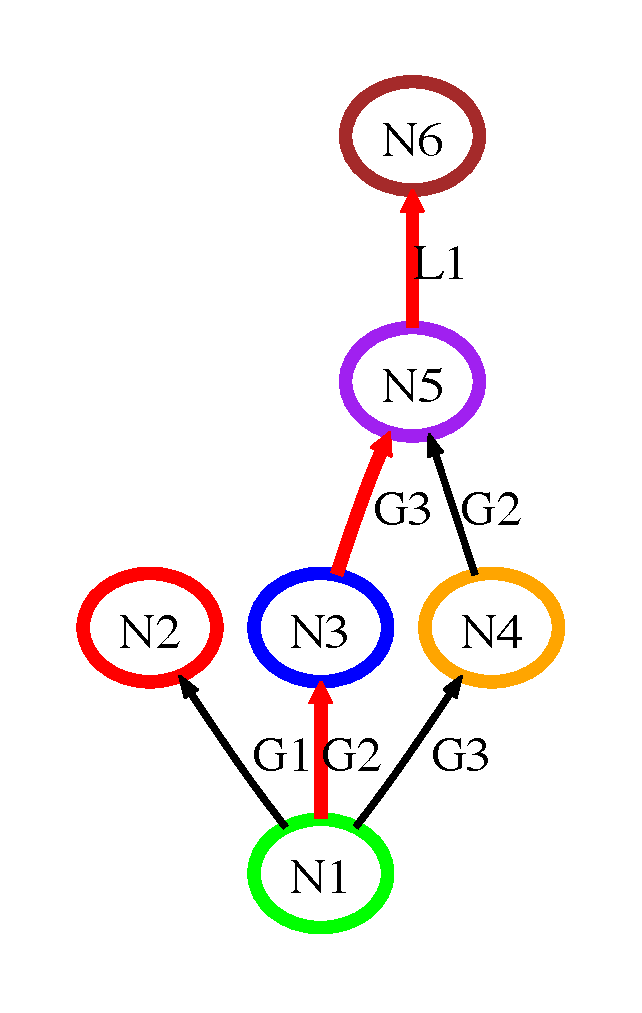
\includegraphics[height=0.22\textwidth]{figs/full_mushroom_cgraph.pdf} 

 % b)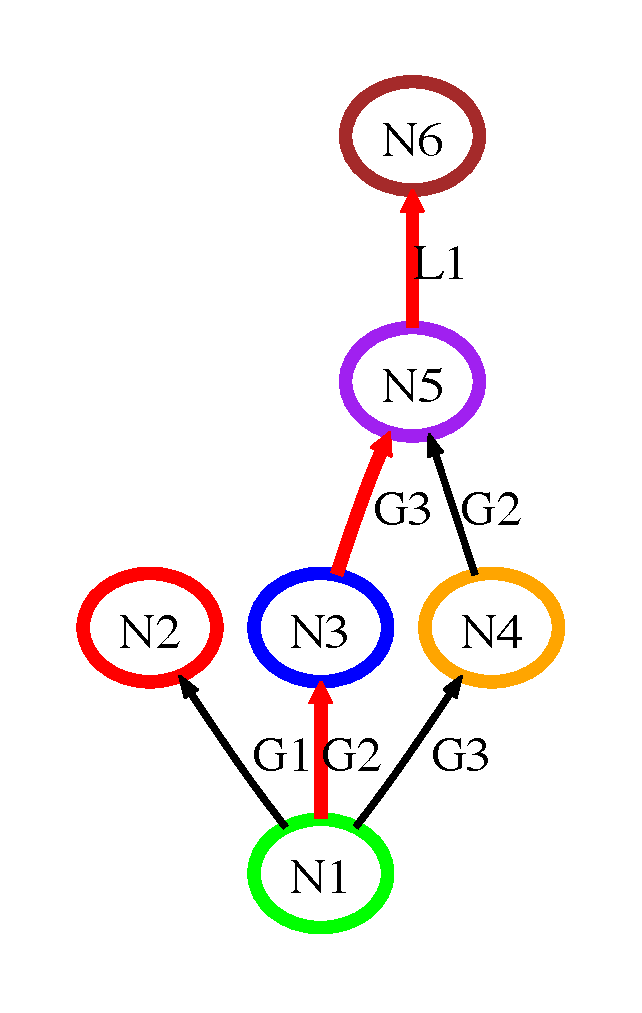
\includegraphics[height=0.25\textwidth]{figs/full_mushroom_cgraph.pdf}
\caption{Transform dynamics reduces the search space by comparing two three transform sequence examples of Figure~\ref{fig:snake_seq} having zero dependency factor and Figure~\ref{fig:mushroom_seq} having dependency factor of one. Observe how the search tree for Figure~\ref{fig:snake_seq} requires 16 nodes, shown in (a) while the search tree for Figure~\ref{fig:mushroom_seq} requires only 8 nodes, shown in (b). When redundancy due to transform order independence is taken into account the savings are from 8 nodes in (c) collapsed from the 16 nodes of (a) to 6 nodes in (d) collapsed from the 8 nodes of (b), respectively. }
  %% \caption{a) Three independent transforms represented as disconnected blue nodes. b) Three transforms that have pairwise dependencies for Figure~\ref{fig:mushroom_seq}. c) The search space represented as a tree for (a). d) The search space represented as a tree for (b). Observe the differences in nodes between (a) and (b). The \textcolor{red}{red} path in the tree, represents $Seq_1$ explored in Figure~\ref{fig:mushroom_seq}. e) The graph structure after capturing redundancy from (c). f) The graph structure after capturing redundancy for (d). The same path is highlighted \textcolor{red}{red} in the graph structure. }
  \label{fig:seq_cgraphs2}
\end{figure}
 
This \emph{dependency factor}, typically one to four, has a dramatic effect on both the complexity and representation of our search space. Figure~\ref{fig:seq_cgraphs2} illustrates how transform dynamics reduces the expected search space, by comparing the full search spaces corresponding to the three-transform sequences of Figure~\ref{fig:snake_seq}, which has a dependency factor of zero, \ie, no transform dynamics effects as shown in Figure~\ref{fig:seq_cgraphs2}\textcolor{red}{(a)}, and of Figure~\ref{fig:mushroom_seq}, which has a dependency factor of one as shown in Figure~\ref{fig:seq_cgraphs2}\textcolor{red}{(b)}. Observe how the search spaces reduce from 16 nodes to 8 nodes. When transform order independence is taken into account as well, the search tree in Figure~\ref{fig:seq_cgraphs2}\textcolor{red}{(a)} collapses to an 8 node graph, Figure~\ref{fig:seq_cgraphs2}\textcolor{red}{(c)}, in contrast to Figure~\ref{fig:seq_cgraphs2}\textcolor{red}{(b)} which collapses to a 6-node graph, Figure~\ref{fig:seq_cgraphs2}\textcolor{red}{(d)}. Quantifying the computational savings due to transform dynamics is difficult to formulate in closed form. 


%% Except for trivial computational savings is difficult to quantify in closed form, but empirically we have observed a huge reduction in our search space.% See the Appendix for further details. 


%% being rendered impossible, and also the formation of new sequences outside of the original set. In practice, the number of candidate transforms that are disqualified as a result of a recently applied transform is overwhelmingly more than the number of newly introduced transforms.  

%% To understand the effect of transform dynamics on our search space more formally we can define the notion of a \emph{dependency graph}. Given $N$ detected transforms this graph captures how the application of a single transform affects the other $N-1$ transforms.  If we revisit Figure~\ref{fig:mushroom_seq}, the dependency graph for this simple example as represented by adjacency matrix is 

%% \begin{equation}
%% Depend_{graph}=\bordermatrix{~ & G_1 & G_2 & G_3 \cr
%%   G_1 & 0 & 1 & 1 \cr
%%   G_2 & 1 & 0 & 0 \cr
%%   G_3 & 1 & 0 & 0 \cr}
%% \label{eq:depend_graph}
%% \end{equation}

%% Each row or column represents one particular transform and entries within the matrix capture independent (zero) neighbors or dependent (one) neighborhood relationships. Observe how with this simple example the application of any single transform is connected to at most two other dependent transforms \ie the application of one transform disqualifies the application of another one to two transforms. By computing the dependency graph over many images, Figure~\ref{fig:cluster}\textcolor{red}{c,f}, we observe that on average the application of any transform (\textcolor{blue}{blue} nodes)


%% To understand the effect of transform dynamics on our search space we observe how it changes for different \emph{dependency factors}. In the previous examples, Figure~\ref{fig:snake_seq} and Figure~\ref{fig:mushroom_seq}, a set of three transforms were initially detected where each set has a different pairwise relationship. Figure~\ref{fig:seq_cgraphs2}\textcolor{red}{(a)} captures the relationship of the three transforms in Figure~\ref{fig:snake_seq} as three disconnected nodes, \ie, a \emph{dependency factor} of zero. In contrast, Figure~\ref{fig:mushroom_seq} leads to a relationship, Figure~\ref{fig:seq_cgraphs2}\textcolor{red}{(b)}, where one transform is connected to two other transforms while the other transforms have a \emph{dependency factor} of one. Figures~\ref{fig:seq_cgraphs2}\textcolor{red}{(c)} and \ref{fig:seq_cgraphs2}\textcolor{red}{(d)} show the search space for the pairwise relationships captured in \textcolor{red}{(a)} and \textcolor{red}{(b)} respectively. Notice that due to transform dynamics the search space is significantly smaller, 8 nodes, as compared to the search space when the \emph{dependency factor} is zero, 16 nodes. If we couple this with capturing redundant transform sequences we reduce our search space from 16 to 8, \textcolor{red}{(c)} to \textcolor{red}{(e)}, and 8 to 6, \textcolor{red}{(d)} to \textcolor{red}{(e)}. In this case, the majority of computational savings was due to transform dynamics (16 to 8 nodes) rather than capturing redundancy (8 to 6 nodes). We note that both these reductions are independent of each other and the effect of both whether applied together or individually is greater the larger the number of transforms. Quantifying the computational savings due to transform dynamics is difficult to formulate in closed form. 

%% As we explore transform sequences the \emph{dependency factor} can vary after application of each individual transform. 


%% Observe also that is difficult to formulate the reduction effect of dynamic transforms through a formula. 



%% Comparing Figure~\ref{fig:seq_cgraphs2}\textcolor{red}{(b)} which models three independent transforms to Figure~\ref{fig:seq_cgraphs2}\textcolor{red}{(c)} we observe the dramatic reduction in the search space from 15 to 8 transforms due to 



%% We observe how these different \emph{dependency factors} leads to very different search spaces, Figure~\ref{fig:

%% We observe in Figure~\ref{fig:seq_cgraphs2} how the structure of the search space changes when we have a set of transforms whose relationship is defined by Equation~\ref{eq:depend_graph}.  If all three transforms were independent (not conflicting) then we would end up with an identical search space to Figure~\ref{fig:seq_cgraphs}\textcolor{red}{a}. However, given that $G_1$,$G_2$, and $G_3$ nullify the application of another one to two transforms leads to the representation, Figure~\ref{fig:seq_cgraphs}\textcolor{red}{a}, where the original fifteen node tree tree has been reduced to eight nodes.


%% The majority of computational savings in this case is not from catching redundancies, but rather in the original search space itself as the size of Figure~\ref{fig:seq_cgraphs2}\textcolor{red}{a} is half the size of Figure~\ref{fig:seq_cgraphs}\textcolor{red}{a}! 


%% The implication of this is that our new upper bound of the search space, Equation~\ref{eq:complexity2} is overly conservative as it assumes that all combinations of $N$ transforms are possible. Looking at Figure~\ref{fig:seq_cgraphs2}\textcolor{red}{b} we see that not all combinations of the original set of three transforms,$G_1$,$G_2$, and $G_3$, are possible, leading to only five transform sequences to consider. 

%% However, Equation~\ref{eq:complexity2} predicts that for three transforms there are seven transform sequences to consider.


%%  Even more the path of  $N_1 \xrightarrow[]{G_2} N_3 \xrightarrow[]{G_3} N_5$ leads to the introduction of a new transform, $L_1$, which is impossible to predict with Equation~\ref{eq:complexity2}. Given that is very difficult to model the interdependencies between transforms and hence the exact size of our search space, we continue to look for ways to tighten our upper bound as we have done moving from Equation~\ref{eq:complexity} to Equation~\ref{eq:complexity2}. 


 %% In practice, we {\bf DO NOT} compute this graph, as it requires the pairwise comparison of all N transforms which is quadratic in the number of transforms.  

%% Our analysis of the search space so far has been purely a function of the number of transforms. This analysis ignores the latent variable of configuration: how does the spatial layout of transforms affect the search space? In the previous example, Figure~\ref{fig:seq_cgraphs}, all transforms were spatially distributed such that they were all independent, \emph{i.e.} the application of one transform doesn't exclude the execution of another transform. In contrast, Figure~\ref{fig:mushroom_seq} depicts the situation of a set of transforms where the application of a transform results in some sequences never happening, and also the formation of new sequences outside of the original set. Intuitively the closer transforms are to each other the more likely they will be dependent.
%% Figure~\ref{fig:seq_cgraphs2} shows how the structure of the search space changes when we have a conflicting set of transforms.  If all three transforms were independent (not conflicting) then we would end up with an identical search space to Figure~\ref{fig:seq_cgraphs}\textcolor{red}{a}, and by consequence the same computational savings and graph structure depicted in Figure~\ref{fig:seq_cgraphs}\textcolor{red}{b}. The majority of computational savings in this case is not from catching redundancies, but rather in the original search space itself as the size of Figure~\ref{fig:seq_cgraphs2}\textcolor{red}{a} is half the size of Figure~\ref{fig:seq_cgraphs}\textcolor{red}{a}! The implication of this is that our new upper bound of the search space, Equation~\ref{eq:complexity2} is overly conservative as it assumes that all combinations of $N$ transforms are possible. Looking at Figure~\ref{fig:seq_cgraphs2}\textcolor{red}{b} we see that not all combinations of the original set of three transforms,$G_1$,$G_2$, and $G_3$, are possible, leading to only five transform sequences to consider. However, Equation~\ref{eq:complexity2} predicts that for three transforms there are seven transform sequences to consider. Even more the path of  $N_1 \xrightarrow[]{G_2} N_3 \xrightarrow[]{G_3} N_5$ leads to the introduction of a new transform, $L_1$, which is impossible to predict with Equation~\ref{eq:complexity2}. Given that is very difficult to model the interdependencies between transforms and hence the exact size of our search space, we continue to look for ways to tighten our upper bound as we have done moving from Equation~\ref{eq:complexity} to Equation~\ref{eq:complexity2}. 



%% The effect of a dynamic search space is not confined to just an adjustment in our complexity analysis, but it also necessitates exploring many alternative paths.  Since we don't know a priori which transform sequences will lead to dead-ends and which will lead to new transforms, we have to explore a large portion of our search space. It is this dynamic nature of our search space, that leads to an exhaustive exploration of all transform sequences. For example, revisiting Figure~\ref{fig:seq_cgraphs2}\textcolor{red}{f}, Node $N_1$ presents us with three possibilities, either explore the path to $N_2$ or $N_3$ or $N_4$. Not all these path leads to the full object (mushroom in Figure~\ref{fig:mushroom_seq}) but there is no way to know that at the start of our algorithm. However, if we assumed all transforms were independent and no new transforms developed then theoretically we would have to explore just one path as all lead to the same final representation. A side-effect of this is we produce a wide variety of object proposals, both nonsensical and veridical. By exploring many mutually exclusive alternative sequences, and not greedily committing to just one or a few paths we increase our likelihood of finding meaningful object proposals in our search space.

%% \noindent\\
%% {\bf Reduction through Transform Independence and Clustering} As previously discussed the high dependency of transforms automatically prunes our search space by discarding impossible sequences. The effect of transform dynamics is not limited to pruning out dependent transform sequences, but it also allows for us to discard combinations of transforms that do not affect each other. Observe that in the previous figure, Figure~\ref{fig:cluster}\textcolor{red}{c,f}, that many nodes of the graph are {\bf NOT} connected to other transforms. Furthermore, whole subgraphs are disconnected, as shown by the graph structure on the upper flower, Figure~\ref{fig:cluster}\textcolor{red}{c} and background zebra, Figure~\ref{fig:cluster}\textcolor{red}{f}. If all transforms were dependent then every node of the graph would be connected to every other node. From the adjacency matrix perspective this is reflected in the sparseness of the matrix, Equation~\ref{eq:depend_graph}. This implicit partitioning of transforms across the image can be exploited by dividing the space of transforms into subsets of dependents transforms that can be exclusively explored without considering the expensive cross product of all combinations of transforms. 

%% Two issues arise in practically implementing the idea of clustering by mutually independent transforms. First, to optimally determine sets of independent transforms we need to compute a dependency graph which as we discussed earlier poses a significant computational burden due its quadratic complexity, defeating the purpose of reducing the search space. Observe, however, that nodes (transform) of the graph that are spatially close tend to be dependent while transforms that are spatially distant are independent.  The implication of this is that the effect of a transform is spatially limited and only affects transforms within a small neighborhood. We can exploit this property by running a standard clustering algorithm that generates clusters by maximizing spatial proximity, Figure~\ref{fig:cluster}\textcolor{red}{g}. These clusters roughly correspond to highly connected subgraphs of the dependency graph. While we could run this cycle every time of detecting transforms and running a clustering algorithm it poses another computational burden as clustering algorithms are computational expensive and sensitive to initialization.  To overcome this second issue we need to effectively spatially partition the space of transform sequences by some other means.

%% There are many ways to achieve this partitioning. For example, we could divide the image into squares, and treat all transforms within the squares as independent sets. Another way, is to cluster all transforms within some neighborhood of a contour as independent sets. We could also equivalently cluster transforms by grouping all those affecting an MVF, Figure~\ref{fig:cluster}\textcolor{red}{h}. Observe that each fragment is associated with a variable number of transforms that tend to overlap the closer in proximity the fragments are. This fragment-centric approach is attractive because what we seek is not a sequence of transforms but the result of what a sequence of transforms can do. By spatially focusing attention on a fragment and then maintaining that focus we are more likely to generate meaningful groupings. Specifically, in this paradigm, the image contains some number of spatially distributed seed fragments, say $M$. In practice, these seeds are determined by simple heuristics, which we discuss in the Experiments section. Figure~\ref{fig:cluster}\textcolor{red}{e} shows the set of all transforms for the image and the reduced set of transforms, Figure~\ref{fig:cluster}\textcolor{red}{j}, indexed by the three seed fragments, $F_1$,$F_2$,and $F_3$. Computationally, this indexing is simple as the contours that bound a medial visual fragment participate in contour-based transforms and the region participates in region-based transforms. Given these initial set of transforms associated with each of the seed fragments we observe three length two sequences, Figure~\ref{fig:cluster}\textcolor{red}{k,l}. Notice that the effect of these sequences is limited to the area defined by the seed fragment. By expanding from seed medial visual fragments we have effectively partitioned the search space to exclusively focus on exploring these independent sets of fragment specific transforms. 



%% If we observe the growth of Equation~\ref{eq:complexity3} in Figure~\ref{fig:frag_growth_redun} we notice that the larger the number of clusters (seed MVF) $M$ the higher the savings. Formula~\ref{eq:complexity} represents a very conservative estimate of the computational savings as we assume that each individual fragment indexes distinct subsets of the original set of $N$ transforms. In practice, many fragments especially those that are spatially close overlap with the subset of transforms they consider, and also the number of indexed fragments is variable, Figure~\ref{fig:cluster}\textcolor{red}{h}. Just as we see a huge reduction in the number of transform sequences from Equation~\ref{eq:complexity2} to Equation~\ref{eq:complexity3} the structure of our representation has changed again. By enforcing locality we end up with many root nodes and move further away from a tree to a more general graph. From where we started a search space represented as a tree defined by Equation~\ref{eq:complexity} we are now at a general graph where the number of sequences to consider is bounded by Equation~\ref{eq:complexity3}. Finally, another just as important savings is that by moving to a local approach we reduce the time to detect transforms as this process can now be confined to a local window rather than the whole image.  

%% \begin{figure}[ht]
%%   \centering
%%   a)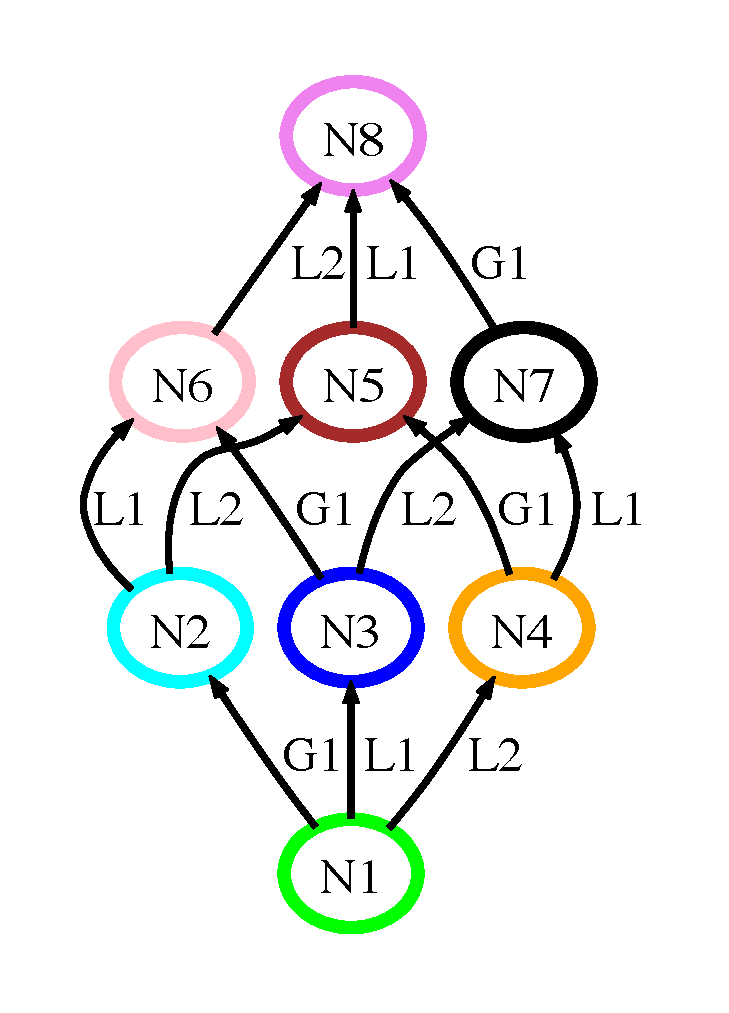
\includegraphics[height=0.25\textwidth]{figs/fish_cgraph_global.pdf} 
%%   b)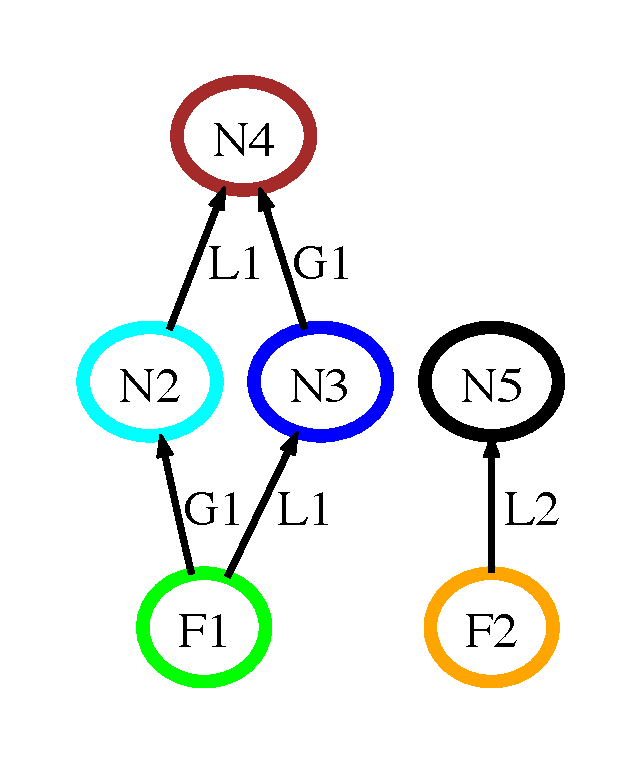
\includegraphics[height=0.22\textwidth]{figs/fish_cgraph_local.pdf}
%%   \caption{If we were to consider a global approach to Figure~\ref{fig:fish_seq}\textcolor{red}{a} the graph would look like a). If we consider a local approach the graph would look like b).   }
%%   \label{fig:fish_cgraphs}
%% \end{figure}


%% The size of this graph, number of edges and nodes, reflects how much of the search space we want to explore. Even if it was possible to explore all transform sequences, it would be unnecessary as not all paths are plausible.
 
\noindent\\{\bf IV Reduction through Discarding Unlikely Sequences: } Despite the significant reduction in the exponential growth of the search space with respect to the number of transforms as enumerated above, the search of the reduced space remains impractically expensive, except in the simplest of scenes.  There are two main underlying reasons. First, there are a vast number of highly unlikely, but possible, transform sequences in the search space. Second, the size of the search space is vastly smaller, and more manageable, if the aim is to recover object parts, than it is recover whole objects. The highly unlikely sequences can be discarded by developing a notion of how likely a transform sequence is. The second goal can be achieved by simply limiting the exploration of transform sequences which have fallen below a certain likelihood. 


%% The goal of this section is to formulate a notion of likelihood for transform sequences and given a fixed computational budget, to consider all transform sequences matching that budget. 

%% \textcolor{red}{[To Ben: I really don't understand what you are saying here in this paragraph, some of your edits were visually a little unclear]} 

The likelihood of a transform sequence, $(T_1,T_2,\cdots,T_N)$, assuming transforms are independent of each other is 

\begin{equation}
p(T_1,T_2,\cdots,T_N)=\prod_i^Np(T_i)
\label{eq:path_like}
\end{equation}

\noindent
where $p(T_i)$ represents the likelihood of a transform $T_i$. At first glance, we can simply ask that any sequence whose likelihood drops below a threshold $P_o$ ($P_o=0.05$) is no longer explored. This is illustrated in Figure~\ref{fig:cgraph_limit} where paths at nodes which fall below threshold are no longer expanded. This implies that each individual transform must have likelihood exceeding $P_o$, \ie, $p(T_i) \geq P_o$, $\forall i$. Second, we have experimentally found that veridical sequences rarely have one transform that has poor likelihood and all other transforms that feature nearly certain likelihood. Thus, a second threshold $P_1$ ($P_1=0.075$) can be placed on each transform as well. This is illustrated by the ``unexplored node'' indicated as dashed circle in Figure~\ref{fig:cgraph_limit}, where $p(T_4)=0.07 \le P_1$. 

\begin{figure}[ht]
  \centering
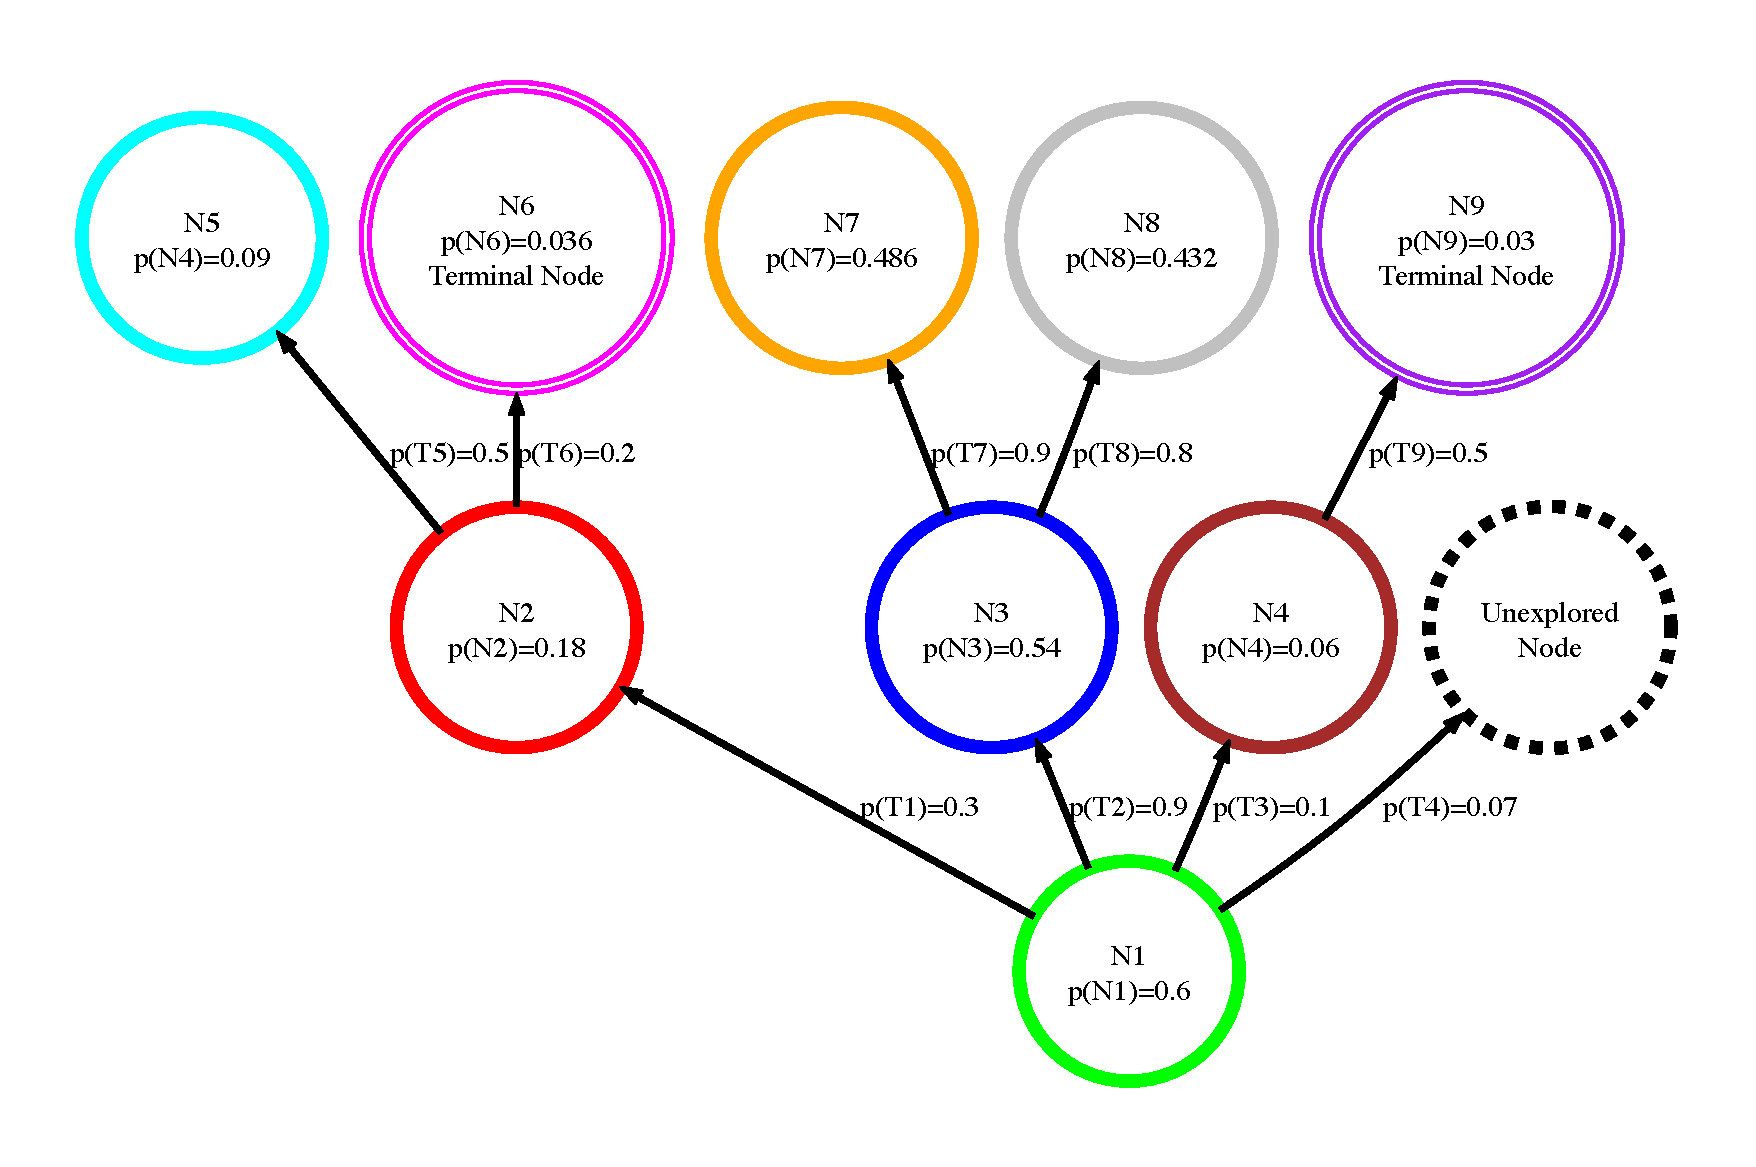
\includegraphics[width=0.30\textwidth]{figs/cgraph_cost.pdf}

  %% a)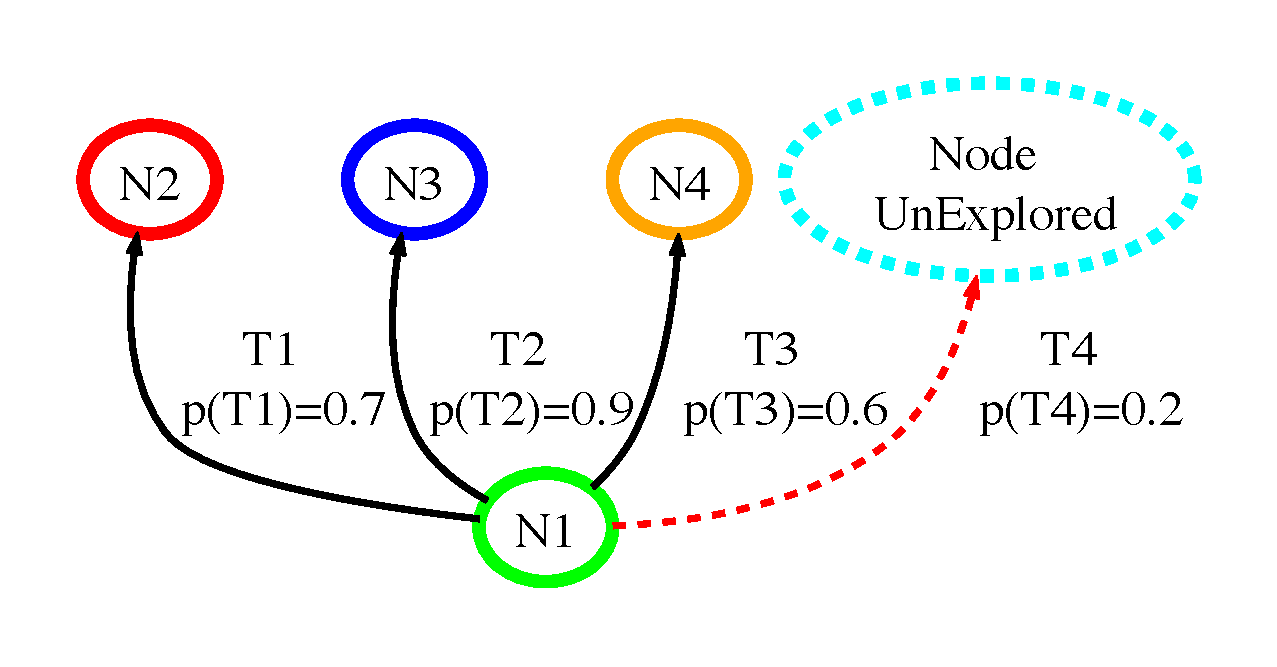
\includegraphics[height=0.15\textwidth]{figs/transform_threshold.pdf} 
  %% b)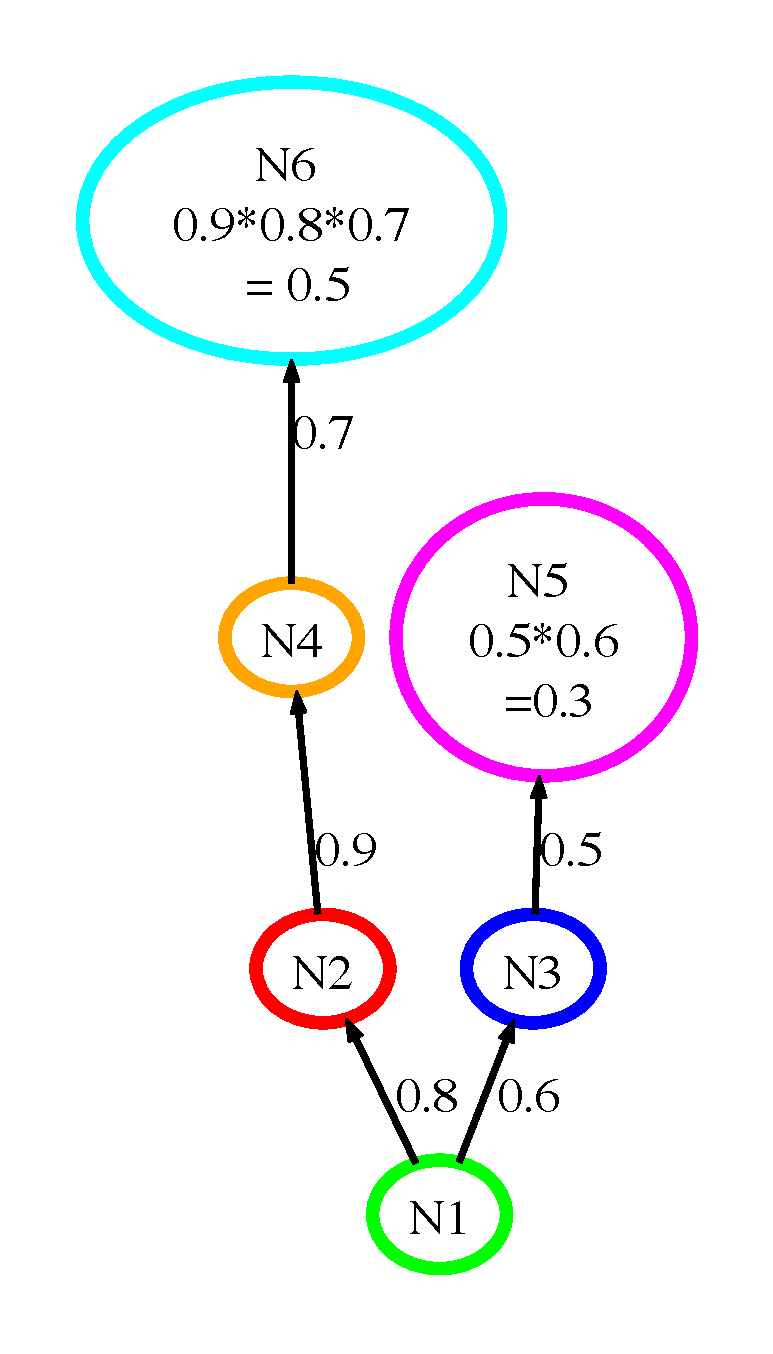
\includegraphics[height=0.20\textwidth]{figs/path_threshold.pdf}
  \caption{Limiting sequence likelihood prunes the search space in two ways: \emph{(i)} Each transform sequence likelihood overall should be above $P_o=0.05$ and \emph{(ii)} each individual transform mush have likelihood exceeding $P_1=0.075$.}
  \label{fig:cgraph_limit}
\end{figure}

An alternate strategy is to observe that for veridical sequences of transforms the likelihood of a path drops with the number of transforms, Figure~\ref{fig:seq_vs_N}\textcolor{red}{(a)}. Stated differently, among all veridical transform sequences, we expect longer sequences to have lower likelihood. In this second model, we assume that the likelihood of a sequence of length $N$ drops exponentially, thus we can define a threshold that is length dependent, \ie, threshold of likelihood of a sequence of length $N$ needs to be greater or equal to $P_N=P_o(P_1)^N$ where $P_o$ and $P_1$ model this distribution. For example with $P_o=1$ and $P_1=0.8$ the threshold at transform sequence length of 8, 25, and 40 would be 0.05, 0.02, and 0.01 respectively. We have not implemented this approach.                                 

%% We select a threshold $p_o$, typically $p_o=0.075$, where we explore further from any transform sequence $(T_1,T_2\cdots,T_N)$ for which $p(T_1,T_2,\cdots,T_N) \geq p_o$. This immediately implies that the likelihood of each individual transform $p(T_i) \geq P_o$. \textcolor{red}{[To Ben: What does wider spread mean in the upcoming sentence? ]} In order to ensure a wider spread of transform sequences, reflecting an expectation that the likelihood of a transform sequence is expected to drop with increasing the number of transforms in a sequence. Ideally, we could have a strategy where $p(T_1,T_2,\cdots,T_N) \ge p_N$, where $p_N=p_op_{exp}^N$, where $p_{exp}$ is the average expected probability of a good transform sequence; we use $p_{exp}=0.80$. This means that at 8 transforms the threshold is at 0.05, at 2.5 transforms it is at 0.02, and at 40 transforms is at 0.01, with the expectation that each individual transform has $p \geq p_o$, Figure~\ref{fig:seq_vs_N}\textcolor{red}{(a)}. \textcolor{red}{[To Ben: are you saying there is only one threshold? Are we getting rid of Figure~\ref{fig:cgraph_limit} ? I am fine with that]}


\begin{figure}[ht]
\centering
{\footnotesize\textit{\textcolor{black}{a)}}}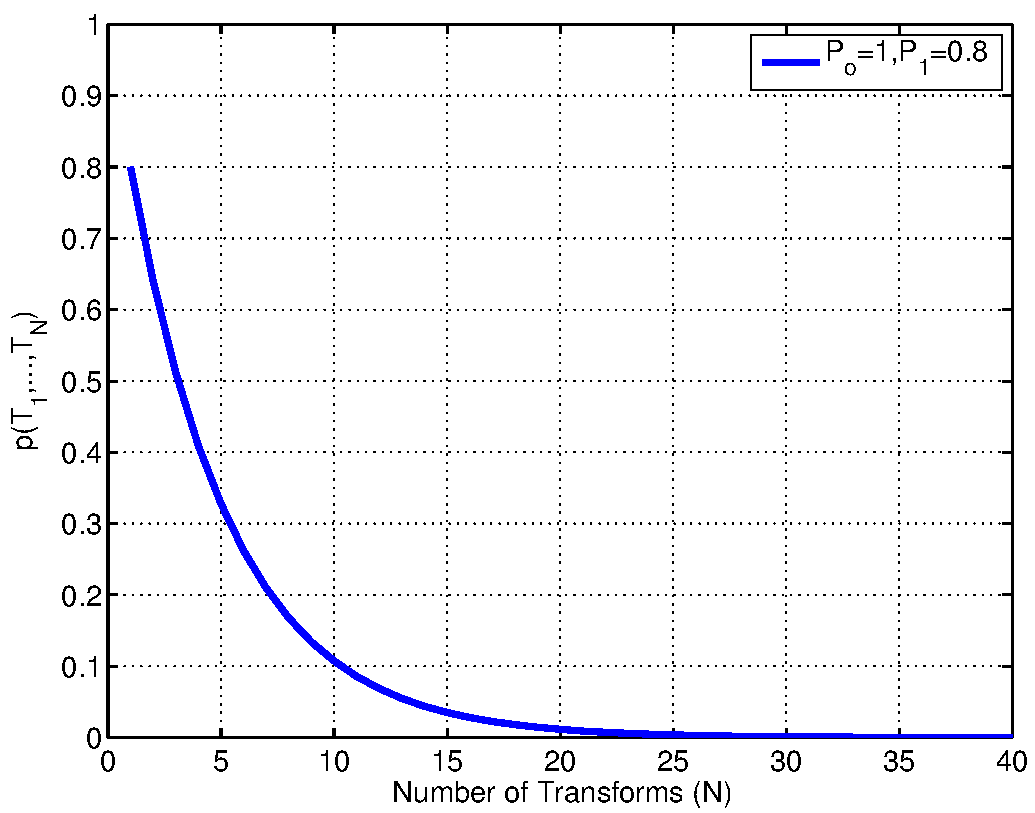
\includegraphics[width=0.22\textwidth]{figs/p_vs_N.pdf}
{\footnotesize\textit{\textcolor{black}{b)}}}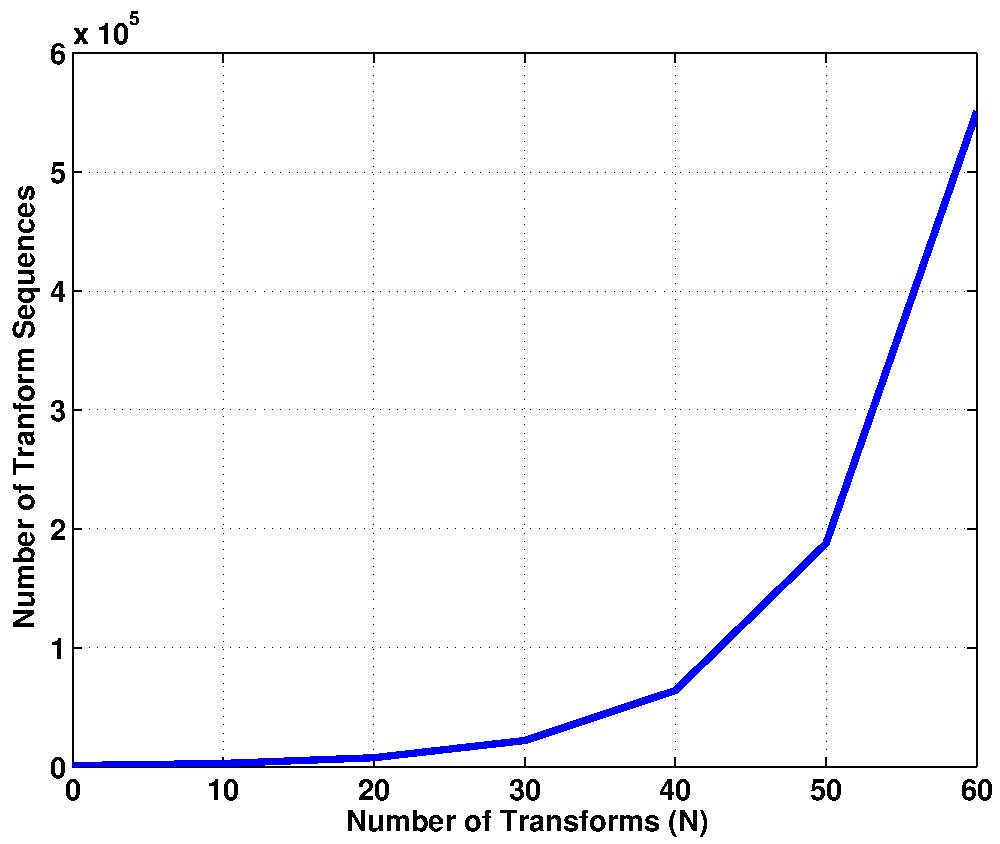
\includegraphics[width=0.22\textwidth]{figs/cost_savings.pdf}
\caption{a) We observe the probability of a transform sequence dropping with $N$ according to Equation $P_N=P_o(P_1)^N$, where $P_o=1$ and $P_1=0.8$. (b) We quantify the computational savings of enforcing a likelihood constraint on our system. }
\label{fig:seq_vs_N}
\end{figure}


The restriction of the search space by limiting transform likelihood is crucial to its practical implementation. Figure~\ref{fig:seq_vs_N}\textcolor{red}{(b)} shows how the search space with the above likelihood constraint grows with the number of transforms. 


\noindent\\
{\bf Containment Graph:} It is clear from the discussions therefore that an effective model of the search space for the space of transform sequences is a weighted graph which can now be formally defined: 



%% The association of a likelihood for any path gives a weight to each node so that the state space becomes a weighted graph:


%% By thresholding the likelihood of each individual transform, $p(T_i)$, and capping the likelihood of a transform sequence as defined in Equation~\ref{eq:path_like} we limit the exploration of highly unlikely transforms and transform sequences. The coupled effect of this, is that each individual node only expands (outgoing edges) to a set of transforms with high probability, while the depth of the graph is curtailed by the creation of many terminal nodes, Figure~\ref{fig:cgraph_limit}. By restricting exploration at each node to only a set of highly likely transforms our scheme mirrors the classic \emph{beam search} algorithm in computer science. Briefly, given a node in a search tree beam search generates and retains the $N$ most promising successor states and subsequently expands the most promising node in this limited set while searching for a goal state. In contrast to beam search where the the number of successor states are fixed, ours is variable depending on how many transforms are above threshold. Even more we utilize our approach to explore many alternative paths with no clearly defined goal state or optimal solution.  


%% The previous examples showed how our search space can be pruned by merging redundant transform sequences while further reductions can be achieved by considering multiple local searches rather than a more global approach. How can we achieve further computational savings? The steps we have taken so far were based on intrinsic properties of transform sequences, but another and just as important cue is based on external evidence, \ie image evidence. Even if it was possible to explore all transform sequences, it would be unnecessary as not all paths are likely \ie have strong image evidence. This property is captured for individual transforms by their associated cost. How can we achieve the same for transform sequences? We consider plausible transform sequences those that are spatially close, and have a high likelihood of being veridical. The former is achieved by expanding from medial visual fragments, while the latter is based on restricting our search space to individual transforms and transform sequences that are highly probable. Assuming independence of transforms, the likelihood of a transform sequence is





%% How does this latest reduction step affect the complexity and structure of the search space? By limiting exploration of the search space to highly plausible transform sequences we observe significantly fewer nodes to visit and drastic reductions in the number of paths that we need to explore. The latter is difficult to quantify as no reasonable assumptions can be made to simplify Equation~\ref{eq:complexity3} any further. Despite this we have empirically observed huge computational savings, as we are in practice unable to run the algorithm without this step! Lastly, just like previous steps our representation of the search space changes from a directed graph to a weighted directed graph with each edge augmented with its transform cost and each node augmented with its cumulative probability, Equation~\ref{eq:path_like}. Nodes of the graph that have multiple incoming paths are attached a single likelihood which is the same irregardless of the transform sequences traversed to get there. For example, reaching node $N_4$ in Figure~\ref{fig:fish_cgraphs} has an identical likelihood, $P(G_1,L_1) == P(L_1,G_1)$, irregardless of which of the two possible paths were traversed. 


%% In summary, the effect of all our reduction steps has evolved our upper bound from Equation~\ref{eq:complexity} to Equation~\ref{eq:complexity2} and finally Equation~\ref{eq:complexity3}. Our search space is still exponential but have we drastically reduced the rate of growth of our space as a function of the number of transforms. Just as our complexity has evolved, so two has our representation of the space. From an initial search tree we are now at a weighted directed graph. We refer to this representation of our search space as the \emph{containment graph}, Definition~\ref{def:cgraph}.

\begin{definition}
The \emph{containment graph} is a weighted directed graph $G=(V,E)$, where each node, $v \in V$, represents the state space, namely the RECOIN representation, coupled with a likelihood for each node which is defined to be the minimum likelihood of all paths terminating there. Each graph link, $e \in E$, represents a transform with an associated likelihood. The containment graph encapsulates all our previous reduction steps in one data-structure.


%% captures our layered representation coupled with a likelihood, and each link represents an applicable transform ( contour-completion, contour clutter removal, etc) and its associated likelihood. A directed path in this graph represents a transform sequence. The containment graph represents the search space, namely the space of all {\bf explored} transform sequences. %% \textcolor{red}{To Ben: Subtle but important point here , the cgraph represents only what we explored, NOT the full search space, } 
\label{def:cgraph}
\end{definition}

\noindent
The containment graph represents the search space, namely the space of all transform sequences. Nodes with multiple incoming links in the graph represent redundant transform sequences converging to identical states. Weights attached to links and nodes, capture how plausible individual transforms and sequences are. Finally, expanding from seed MVF nodes restricts the search to be local, Figure~\ref{fig:cgraph_abstract}. Figures~\ref{fig:seq_cgraphs2}\textcolor{red}{(e,f)} represent other examples of a containment graph. 


\begin{figure}[ht]
\centering
{\footnotesize\textit{(a)}}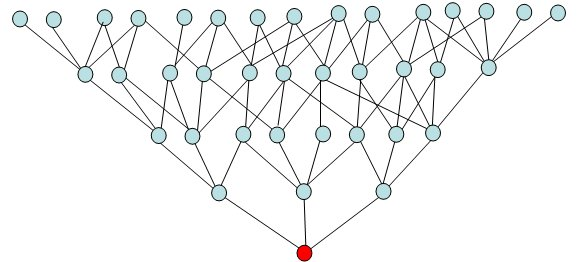
\includegraphics[width=0.25\textwidth]{figs/hypothesis-tree.jpg}
{\footnotesize\textit{(b)}}\includegraphics[width=0.35\textwidth]{figs/merged-hypothesis-trees.jpg}
\caption{A high level abstraction of the containment graph (a) The graph of grouping possibilities involving a single fragment. (b) The union of  graphs  from all fragments is the   {\bf containment graph}.}
\label{fig:cgraph_abstract}
\end{figure}

\begin{figure*}[p]
\centering
\setlength{\fboxsep}{0.0005mm}
\setlength{\fboxrule}{4pt}
a) \raisebox{-0.1\height}{\includegraphics[width=0.25\textwidth]{figs/cgraph.pdf}}
b)\fcolorbox{green}{white}{\includegraphics[width=0.140\textwidth]{figs/n1.pdf}}
\fcolorbox{red}{white}{\includegraphics[width=0.140\textwidth]{figs/n2.pdf}}
\fcolorbox{blue}{white}{\includegraphics[width=0.140\textwidth]{figs/n3.pdf}}
\fcolorbox{cyan}{white}{\includegraphics[width=0.140\textwidth]{figs/n4.pdf}}
\fcolorbox{magenta}{white}{\includegraphics[width=0.140\textwidth]{figs/n5.pdf}}
\fcolorbox{orange}{white}{\includegraphics[width=0.140\textwidth]{figs/n6.pdf}}
\fcolorbox{black}{white}{\includegraphics[width=0.140\textwidth]{figs/n7.pdf}}
\fcolorbox{purple}{white}{\includegraphics[width=0.140\textwidth]{figs/n8.pdf}}
\fcolorbox{gray}{white}{\includegraphics[width=0.140\textwidth]{figs/n9.pdf}}
\fcolorbox{brown}{white}{\includegraphics[width=0.140\textwidth]{figs/n10.pdf}}
c) \raisebox{-0.1\height}{\includegraphics[width=0.27\textwidth]{figs/full_cgraph.pdf}}
d)\fcolorbox{deeppink}{white}{\includegraphics[width=0.140\textwidth]{figs/n1_mvf2.pdf}}
\fcolorbox{tan}{white}{\includegraphics[width=0.140\textwidth]{figs/n11_mvf2.pdf}}
\fcolorbox{darkorange}{white}{\includegraphics[width=0.140\textwidth]{figs/n12_mvf2.pdf}}
\fcolorbox{darkgray}{white}{\includegraphics[width=0.140\textwidth]{figs/n13_mvf2.pdf}}
e) \includegraphics[width=0.09\textwidth]{figs/n1_mvf.png}
\includegraphics[width=0.09\textwidth]{figs/n2_mvf.png}
\includegraphics[width=0.09\textwidth]{figs/n3_mvf.png}
\includegraphics[width=0.09\textwidth]{figs/n4_mvf.png}
\includegraphics[width=0.09\textwidth]{figs/n5_mvf.png}
\includegraphics[width=0.09\textwidth]{figs/n6_mvf.png}
\includegraphics[width=0.09\textwidth]{figs/n7_mvf.png}
\includegraphics[width=0.09\textwidth]{figs/n8_mvf.png}
\includegraphics[width=0.09\textwidth]{figs/n9_mvf.png}
\includegraphics[width=0.09\textwidth]{figs/n10_mvf.png}
f)\includegraphics[width=0.09\textwidth]{figs/n1_mvf2.png}
\includegraphics[width=0.09\textwidth]{figs/n12_mvf2.png}
\includegraphics[width=0.09\textwidth]{figs/n13_mvf2.png}
\includegraphics[width=0.09\textwidth]{figs/n14_mvf2.png}

%% f)\raisebox{0.6\height}{\includegraphics[width=0.14\textwidth]{figs/n1_mvf2.png}}
%% \raisebox{0.6\height}{\includegraphics[width=0.14\textwidth]{figs/n12_mvf2.png}}
%% \raisebox{0.6\height}{\includegraphics[width=0.14\textwidth]{figs/n13_mvf2.png}}
%% \raisebox{0.6\height}{\includegraphics[width=0.14\textwidth]{figs/n14_mvf2.png}}

\caption{The containment graph for a small portion of the image restricted by two nearby seed MVFs. (a) The containment graph restricted to the orange MVF, $N_1$, with all nodes shown in (b). The object proposals corresponding to these 10 nodes are show in (e). (c) The containment graph initiated at a nearby seed MVF, $N_{11}$, as shown in purple, intersects the containment graph in (a). Numerous nodes have already been explored and new nodes are show in (d), with the corresponding object fragments in (f). The contour-based signature discussed in Section~\ref{sec:representation} is documented for each node to highlight the central role this representation plays in the efficient, implementation of our system. }


%% Observe that as we perform contour completion transforms ($G_1$) an extra bit is appended to the string. (c) We observe the corresponding proposals mapping to each of the nodes in the graph. (d) We see the containment graph for another seed MVF (e) indicated as the dashed box. Observe how subsequent seeds visit already previously visited states as indicated by green arrows. Due to keeping tracking of previous state no work is wasted exploring duplicate sequences. (f) We see the object proposals generated by transforming this seed fragment. }

%% Each node in the graph contains a contour-based signature capturing the state of the system. For example, Node $N1$ has a string of ones which means the initial set of all contours are present. Notice that as we apply contour clutter removal transforms ($L_1$,$L_2$) bits are flipped in the string from 1 to 0. }
\label{fig:cgraph_steps}
\end{figure*}



%% \begin{figure*}[hb]
%% \centering
%% %\vspace{-0.61cm}
%% %% \hbox{
%% %% \vbox{
%% %% \hbox{
%% %% {\footnotesize\textit{(a)}}
%% %% \includegraphics[width=0.25\textwidth]{figs/hypothesis-tree.jpg}
%% %% }
%% %% \hbox{
%% %% \hspace{-0.25cm}{\footnotesize\textit{(c)}}\includegraphics[width=0.4\textwidth]{figs/merged-hypothesis-trees.jpg}
%% %% }
%% %% }
%% \includegraphics[width=0.60\textwidth]{figs/elephant.pdf}

%% %\footnotesize\textit{(f)}}  \includegraphics[height=0.1851\textwidth]{figs/containment_graph.pdf}
%%  %{\footnotesize\textit{(c)}}  \includegraphics[height=0.0851\textwidth]{figs/ambiguous-grouping-org.png}
%% %{\footnotesize\textit{(b)}}  \includegraphics[height=0.0851\textwidth]{figs/ambiguous-grouping-1.png}
%% %{\footnotesize\textit{(c)}}  \includegraphics[height=0.0851\textwidth]{figs/ambiguous-grouping-2.png}
%% %\vspace{-0.32cm}
%%   \caption{ An example containment graph for a fragment of an elephant.}
%%   \label{fig:elephant_example}
%%   %\vspace{-0.653cm}
%% \end{figure*}

Figure~\ref{fig:cgraph_steps} illustrates a small but realistic example with transform sequences starting from the seed MVF, node $N_1$ highlighted in light orange. The transforms, namely, contour removal transforms $L_1$ and $L_2$ and a contour completion transform $G_2$ provide three options to transform node $N_1$, Figure~\ref{fig:cgraph_steps}\textcolor{red}{(a)}. The containment graph corresponding to transforms initiated from a different seed MVF, highlighted in purple, $N_{11}$ in Figure~\ref{fig:cgraph_steps}\textcolor{red}{(c)}, very quickly integrate with the containment graph initiated at node $N_1$. The set of all nodes give the object proposals in our framework, Figure~\ref{fig:cgraph_steps}\textcolor{red}{(e,f)}. Two paths which culminate in one node say transform sequences $(L_1,L_2)$ and $(L_2,L_1)$ which end in node $N_6$, Figure~\ref{fig:cgraph_steps}\textcolor{red}{(a)}, have equal likelihood when there are re-ordering of independent transforms. This is intuitively clear: if the formation of a fragment requires the completion of two gaps and removal of three clutter contours, any order of accomplishing these works equally well. If these transforms do not interact the likelihood of all paths to form a node is equal. Otherwise, there is no guarantee that all paths have equal likelihood and the maximum likelihood is adopted. However, since not all paths are explored for efficiency, when there is redundancy, the likelihood is not guaranteed to be accurate, thus some paths may be prematurely terminated. In future, we aim to design transform likelihoods in such a manner that the likelihood of a pair of dependent transform is order independent. Transforms are explored interactively until \emph{(a)} no more transforms are applicable at that node or \emph{(b)} the likelihood of the transform sequence has fallen below threshold. Any partial organization corresponding to a node in the containment graph is an object proposal. Our goal is to organize the image sufficiently that recognizable object parts can be derived. Of course the process may result in the whole object, but this is not our goal for every image.  

\noindent\\
{\bf Construction of the containment graph:} Construction of a containment graph can proceed in a depth-first, breadth-first, or a hybrid traversal approach.  The construction strategy aims to optimize the number of nodes that can be explored in the search space, given a budget of computational processing, core memory, and disc memory constraints.  Let the cost of storing the state of a node be $C_s$ and let the average computational cost be $C_p$. Formally, we seek a strategy that minimizes the total storage cost, $C_S^{Total}$,  and computational run-time, $C_p^{Total}$, as a function of the number of nodes ($N$) in the containment graph. We now examine strategies. 


%% We have already limited the extent of the search space that is explored by limiting the transform sequence likelihood to be above a small threshold.
%% We now examine strategies. 

First, observe that in our framework, transforms can be inverted, \ie, if a transform $T$ takes node $N_6$ to Node $N_9$, the representation retains sufficient information to recover the state of Node $N_6$ solely from the state of node $N_9$. This implies that a depth-first traversal of the tree does not require a storage of the states that are visited because these can be recovered. The computational cost of inverting a transform is identical to implementing the transform. While the states of visited nodes do not need to be stored, this comes at the cost of additional computational resources.  

%% Let the cost of storing the state of a node be $C_s$ and let the cost of processing a transform on average be $C_p$. 


%% Second, an independent set of transforms $(T_1,T_2,…,T_N)$ can be implemented without first having to implement, $T_1$, then $T_2$, and so on to $T_N$. Rather, the sequence can be implemented in one step with significantly reduced computational processing.
%% cost of a processing a transform on average be Cp. Consider an average breadth factor of K and average depth of D and total number of nodes N. 



\begin{figure}[ht]
\center
{\footnotesize\textit{\textcolor{black}{a)}}}\includegraphics[width=0.27\textwidth]{figs/dfs_visit.pdf}
{\footnotesize\textit{\textcolor{black}{b)}}}\includegraphics[width=0.27\textwidth]{figs/bfs_visit.pdf}
{\footnotesize\textit{\textcolor{black}{c)}}}\includegraphics[width=0.35\textwidth]{figs/depth_first.pdf}
\caption{a) We see how a synthetic 7 node containment graph is traversed by a depth-first strategy. The computational cost is roughly proportional to two times the number of nodes with minimal storage requirements. (b) In a breadth first strategy the computational cost is roughly equal to the number of nodes in the graph but at the expense of increased storage. c) The depth-first construction of Figure~\ref{fig:cgraph_steps}\textcolor{red}{(a)}. Observe that previously explored states are not revisited as indicated by the dashed red (N/A) directed links. } 
\label{fig:dfs_traversal}
\end{figure}

The choice of the construction strategy is ultimately a trade off between the use of storage and processing resources. First, consider a depth first construction strategy. Given an MVF seed, and a set of initial transform choices, a transform can be selected and applied. The transform choices for the resulting state are then considered, one transform is selected, and then applied. The process repeats itself until (a) a node is reached where no transforms are applicable or (b) the likelihood of the transform sequence falls below threshold. When this happens, the latest transform is inverted, and the remaining transform at the one to the last node are then considered, Figure~\ref{fig:dfs_traversal}\textcolor{red}{(a)}. Then, each node costs exactly twice the processing cost of a transform, \ie, the total cost is $C^{Total}_p=2(N-1)c_p$ where $N$ is the total number of nodes in the graph. The storage requirements are minimal: only one node needs to be maintained, so total storage is $C_s^{Total}=C_s$. Now consider a breadth-first strategy: a transform from among the transforms at an individual seed node is selected and implemented. The state of the newly explored node is maintained in storage while the remaining transforms are explored in turn. For example if there are three transforms, three new states need to be maintained. For a depth of two, assuming an average branching factor, $K$, of three, more nodes need to be stored, and so on. No transforms need to be inverted, however, Figure~\ref{fig:dfs_traversal}\textcolor{red}{(b)}. The total processing cost is $C_p^{Total}=(N-1)C_p$, while the total storage requirement is $C_s^T=K^D$ where $D$ is the average depth, which is not practical. For this reason we elect to use a depth-first strategy. In future, we aim to design a hybrid traversal strategy that builds on the relative strengths of depth-first (storage) and breadth-first (processing) to reach a compromise between optimizing $C_s^{Total}$ and $C_p^{Total}$.


Figure~\ref{fig:dfs_traversal}\textcolor{red}{(c)} shows how our construction strategy applies to the realistic case in Figure~\ref{fig:cgraph_steps}. Observe that during traversal previously explored states are not revisited. In practice, this implement/invert framework is implemented by a stack where the transforms to be executed are pushed onto to the stack and when they are popped off, the action is inverted. The full algorithm of our exploration is outlined in Algorithm~\ref{algo:overall}.

%% Third, the impractical storage requirements can be alleviated by trading off processing with storage: Each new node takes note of transforms applicable there but does not implement those directly. Rather, all processing is done directly on the seed MFF fragment with moderate storage requirements. For example, the graph in Figure 58(a) can be constructed by first constructing the nodes N2 and N3 as before, but then construct nodes N4, N5, N6, and N7 and directly by implementing the identified transform sequence. The total processing cost is where C^x is the slight requirement of storing identified transforms at each node. 



 

%% continues for a sufficient length the whole object may be inferred but that is not our goal for every image. Now consider the search space when a different fragment is used as the initial point of focus, Figure~\ref{fig:cgraph_steps}\textcolor{red}{(d)}, as highlighted as dark purple in Figure~\ref{fig:cgraph_steps}\textcolor{red}{(e)}. Observe how after a few transforms the transform sequences converge onto those starting from the adjacent fragment $N_1$. This convergence presents an independent growth for each fragment. A second example is given in Figure~\ref{fig:elephant_example}.


%% In this particular example the creation of terminal nodes is due to the former. 
%% Finally, the transformed fragment at each node corresponds to a possible reorganization of the image focused on this initial fragment and therefore constitutes an object part proposal, Figure~\ref{fig:cgraph_steps}\textcolor{red}{(c)}.


%% Observe that the node $N_6$, Figure~\ref{fig:cgraph_steps}\textcolor{red}{(b)}, which corresponds to the removal of contours $L_1$ and $L_2$, can be reached by two sequences $(L_1,L_2)$ and $(L_2,L_1)$, both having the same likelihood. 

%% an initial state focused on transforms applied to a particular fragment, highlighted in light orange. To efficiently keep track of changes to our initial state as we explore sequences we augment each node of the containment graph with the compact binary contour-based signature discussed earlier, Section~\ref{sec:representation}. Initially, all seeds start with a binary string of all ones where the number of ones correspond to the initial number of contours in our representation. Node $N_1$ in Figure~\ref{fig:cgraph_steps}\textcolor{red}{(b)} represents our starting seed under consideration and the specific transforms detected, 

%% \textcolor{red}{To Ben: Wordy yes, but wanted to explain this, can be integrated better} In general, there is no guarantee that the likelihood, Equation~\ref{eq:path_like}, of two order-independent transform sequences will be equal. In practice, however, we assume that the computed likelihoods are invariant to the ordering of transforms. Empirically we have observed that in the vast majority of cases there is a negligible difference between the likelihood of say $p(T_1,T_2)$ versus $p(T_2,T_1)$. If we did not make this approximation we would be forced to explore ALL possible permutations of transforms, thus eliminating the tremendous savings we achieve by exploiting order-independent transforms, Figure~\ref{fig:ss_growth_redun}. For example, in this particular example, for Node $N_6$ we would have to explore both $(L_1,L_2)$ and $(L_2,L_1)$, for Node $N_7$ we would have to explore both $(G_1,L_1)$ and $(L_1,G_1)$, and finally for Node $N_{10}$ all possible incoming paths would have to be explored despite all of them leading to the same transformed state. In general, for any node at any depth (not just length two sequences) in our graph we would have to compute the likelihood of all incoming paths and take the minimum. With our approximation we only have to explore {\bf one} incoming path as we assume the likelihood of any incoming path is equivalent to all the others. Without this approximation the system would be unable to run as the complexity would be equivalent to assuming order-dependent transforms, Equation~\ref{eq:complexity}. A drawback of course, is that our system might prematurely terminate a transform sequence due to likelihood dropping or explore a sequence longer than it should be. 


%% We also observe how the contour-based signatures, annotated by the string inside the nodes in Figure~\ref{fig:cgraph_steps}\textcolor{red}{(a)} change as various transforms are applied. Finally, the containment graph corresponding to node $N_1$ terminates in nodes $N_9$ and $N_{10}$; termination at a node occurs either because 



%% Our approach of limiting the number of options we explore at each node is very similar to the classic \emph{beam search} algorithm in computer science. For a given node in the graph the algorithm generates all possible successor states, $S$, in a breadth first fashion sorted according to some heuristic. However, the algorithm only retains the $N$ most promising states of $S$ and subsequently expands the most promising node in this limited set.  Our approach is similar in that at each node, we restrict the search space to only a set of highly likely set of transforms. In contrast to beam search where the the number of successor states is fixed, ours is variable depending on how many transforms are above threshold. Secondly, the goals of each algorithm are different where beam search is used to find a goal state or optimal solution in a search tree, our approach is predicated on exploring many alternative paths with no clear predefined goal state or optimal solution. 


%% \begin{figure*}[p]
%% \centering
%% \setlength{\fboxsep}{0.0005mm}
%% \setlength{\fboxrule}{4pt}
%% \raisebox{-0.1\height}{\includegraphics[width=0.45\textwidth]{figs/cgraph.pdf}}
%% \fcolorbox{green}{white}{\includegraphics[width=0.23\textwidth]{figs/n1.pdf}}
%% \fcolorbox{red}{white}{\includegraphics[width=0.23\textwidth]{figs/n2.pdf}}
%% \fcolorbox{blue}{white}{\includegraphics[width=0.23\textwidth]{figs/n3.pdf}}
%% \fcolorbox{cyan}{white}{\includegraphics[width=0.23\textwidth]{figs/n4.pdf}}
%% \fcolorbox{magenta}{white}{\includegraphics[width=0.23\textwidth]{figs/n5.pdf}}
%% \fcolorbox{orange}{white}{\includegraphics[width=0.23\textwidth]{figs/n6.pdf}}
%% \fcolorbox{black}{white}{\includegraphics[width=0.23\textwidth]{figs/n7.pdf}}
%% \fcolorbox{purple}{white}{\includegraphics[width=0.23\textwidth]{figs/n8.pdf}}
%% \fcolorbox{gray}{white}{\includegraphics[width=0.23\textwidth]{figs/n9.pdf}}
%% \fcolorbox{brown}{white}{\includegraphics[width=0.23\textwidth]{figs/n10.pdf}}
%% \includegraphics[width=0.095\textwidth]{figs/n1_mvf.png}
%% \includegraphics[width=0.095\textwidth]{figs/n2_mvf.png}
%% \includegraphics[width=0.095\textwidth]{figs/n3_mvf.png}
%% \includegraphics[width=0.095\textwidth]{figs/n4_mvf.png}
%% \includegraphics[width=0.095\textwidth]{figs/n5_mvf.png}
%% \includegraphics[width=0.095\textwidth]{figs/n6_mvf.png}
%% \includegraphics[width=0.095\textwidth]{figs/n7_mvf.png}
%% \includegraphics[width=0.095\textwidth]{figs/n8_mvf.png}
%% \includegraphics[width=0.095\textwidth]{figs/n9_mvf.png}
%% \includegraphics[width=0.095\textwidth]{figs/n10_mvf.png}
%% \caption{The containment graph for a small portion of the image. Expanding from Node $N_1$ we see the nodes explored and their corresponding object proposals. The cost along edges and nodes have been removed from the containment graph for clarity sake. }
%% \label{fig:cgraph_steps}
%% \end{figure*}


%% \begin{figure*}[ht]
%% \centering
%% \setlength{\fboxsep}{0.0005mm}
%% \setlength{\fboxrule}{4pt}
%% \raisebox{-0.1\height}{\includegraphics[width=0.45\textwidth]{figs/full_cgraph.pdf}}
%% \fcolorbox{deeppink}{white}{\includegraphics[width=0.23\textwidth]{figs/n1_mvf2.pdf}}
%% \fcolorbox{tan}{white}{\includegraphics[width=0.23\textwidth]{figs/n11_mvf2.pdf}}
%% \fcolorbox{darkorange}{white}{\includegraphics[width=0.23\textwidth]{figs/n12_mvf2.pdf}}
%% \fcolorbox{darkgray}{white}{\includegraphics[width=0.23\textwidth]{figs/n13_mvf2.pdf}}
%% \raisebox{0.6\height}{\includegraphics[width=0.12\textwidth]{figs/n1_mvf2.png}}
%% \raisebox{0.6\height}{\includegraphics[width=0.12\textwidth]{figs/n12_mvf2.png}}
%% \raisebox{0.6\height}{\includegraphics[width=0.12\textwidth]{figs/n13_mvf2.png}}
%% \raisebox{0.6\height}{\includegraphics[width=0.12\textwidth]{figs/n14_mvf2.png}}

%% %% \begin{tabular}{cc}
%% %% \raisebox{0.4\height}{\includegraphics[width=0.1\textwidth]{figs/n1_mvf2.png} }&
%% %% \raisebox{0.4\height}{\includegraphics[width=0.1\textwidth]{figs/n12_mvf2.png}} \\
%% %% \raisebox{2.3\height}{\includegraphics[width=0.1\textwidth]{figs/n13_mvf2.png}} &
%% %% \raisebox{2.3\height}{\includegraphics[width=0.1\textwidth]{figs/n14_mvf2.png}} \\
%% %% \end{tabular}
%% \caption{Expanding from another seed fragment (dashed box) results in new nodes, but also the formation of many redundant sequences as indicated by the \textcolor{green}{green edges}. }
%% \label{fig:cgraph_steps2}
%% \end{figure*}
 




%% In what follows we show how all these ideas, come together in a more realistic example. Our process, begins by expanding from an initial set of medial visual fragments or seeds. Figure~\ref{fig:cgraph_steps}, highlights one starting fragment from this set and the containment graph that results after some amount of searching.

%% The contour representation of the state is a binary code. 1 means contour is still present while 0 means contour is no longer part of the state. Additional new contours simply add to the representation. 


%% Each node of the containment graph is augmented with a compact signature, namely a variable length binary string encoding the presence or removal of individual contours of our representation. By comparing these compact signature redundant transform sequences can be detected. The intuition behind this approach is that two transformed representations are equivalent if just \emph{one} of the individual layers (contours, shocks, and regions) are identical. Identical shock graph layers, would require an expensive consideration of graph isomorphism to detect equivalency. However, comparing contour sets by this signature is quick, and more importantly changes to this signature amount to simply flipping a character or appending an extra character. For example a binary string of “01” corresponds to a state of 2 contours, $C_1$ and $C_2$, where $C_1$(``0'') has been removed by a transformation while $C_2$ (``1'') still exists. If a gap transform is executed then an extra character is appended to the string corresponding to the addition of a new contour.  All initial seed fragments are represented utilizing an equal length string of size N with all contours encoded to one where N is the number of contours. Returning to our example, we see our local picture is composed of four contours, so Node $N_1$ is represented by a string of four ones.  

%% As discussed earlier, , we can compactly represent our RECOIN representation with a contour-based signature. Briefly, each state or node of the containment graph is augmented with a variable length binary string which encodes the presence (binary 1) or absence (binary 0) of each individual curve in our contour set. Changes to this representation (transforms) amount to flipping bits or extending the string. Equivalency of two states can be achieved by simply comparing two binary strings. In this example, and 




 
%% There are many paths to consider, when expanding from $N_1$ in Figure~\ref{fig:cgraph_steps}. If we start our exploration with $L_2$ our new transformed representation is captured by $N_2$. Notice how our signature has changed to reflect the removal of a contour by flipping a character to zero. If we had instead explored $L_1$, ($N_1 \xrightarrow[]{L_1} N_3$), then this reflect a different contour removed. We see that the removal of both these contours, as captured by Node $N_6$ could have been reached by two distinct paths, ($N_1 \xrightarrow[]{L_1} N_3 \xrightarrow[]{L_2} N_6$) or  ($N_1 \xrightarrow[]{L_2} N_2 \xrightarrow[]{L_1} N_6$), but both result in identical representations. Visiting the last transform under consideration at $N_1$, $G_1$, transforms the representation by inserting a contour and thus expands our string. Continuing further down this path, if we insert another contour, ($N_4 \xrightarrow[]{G_2} N_8$), we see how the signature has increased to a length of 6, reflecting the addition of two contours to our original representation. Finally, Nodes $N_9$ and $N_{10}$ represent terminal nodes in this graph due to either the likelihood of transform sequences dropping below threshold (though not depicted) or possibly no more transforms to explore. The resulting object proposals that would be output can be seen in the bottom row of Figure~\ref{fig:cgraph_steps}. Looking at the output object proposals we observe varying hypotheses, namely some proposals have retained the giraffe spot resulting in the formation of a hole, while others have removed the spot. 

%% We now visit another seed fragment, Figure~\ref{fig:cgraph_steps2}, and illustrate how the search progresses. Node $N_{11}$ proceeds similar to the first seed fragment, but in this case, any new paths are compared to the previously formed containment graph. Expanding from a new seed leads to the creation of new nodes (boxed in Figure~\ref{fig:cgraph_steps2}), but also redundant sequences are merged with the previously explored set of paths as indicated by the \textcolor{green}{green edges}. For example, the path $N_{11} \xrightarrow[]{G_2} N_{12} \xrightarrow[]{G_3} N_8$ was already explored during the search process for the first seed fragment. As we continue to expand from seeds fragments, new nodes are augmented to the graph, but more importantly there is more and more overlap between equivalent transform sequences. Intuitively the closer the seed fragments are the more redundant transform sequences will exist between them, than if they were spread apart across the image. Finally, we show another example of how the containment graph would look like for an image, Figure~\ref{fig:elephant_example}. 


%% {\bf Motivation I (DFS/BFS): } The construction of a containment graph can proceed in a depth-first, breadth-first, or a hybrid traversal approach to optimize storage space, computational efficiency, \etc. Our traversal strategy is motivated by the computational challenges of our approach. The strength of our scheme is we explore many alternative conflicting paths in our search space. The drawback of this approach as compared to a greedy approach, where we could commit to one path, is that we need to efficiently reason with a multitude of conflicting options given our initial representation. A simple strategy to dealing with this is then to keep a separate copy of our RECOIN representation for each conflicting path in the graph. This quickly becomes prohibitive as the containment graph can approach on the order of 70,000 nodes! Rather than explicitly keep a new copy of our representation at each node we can simply recover the transformed state on demand by transforming our initial representation. Observe that in Figure~\ref{fig:cgraph_steps}\textcolor{red}{a} we can recover any single node by simply applying the binary code signature. However, as stated before we don't commit to any one path so after explicitly modifying our representation we must essentially ``undo'' the change before proceeding to another transform. This is trivial given that every transform has a natural converse, \ie, removing a contour can be undone by reinserting the deleted curve. This ``edit/undo'' framework achieves tremendous storage savings as we only need to keep {\bf one} copy of our representation to recover any possible state in our search space! To achieve optimal efficiency, however, we must use a traversal strategy that minimizes the number of edit/undo operations. Figures~\ref{fig:dfs_traversal}\textcolor{red}{(a)} and~\ref{fig:dfs_traversal}\textcolor{red}{(b)} illustrate the ordering of visited links in the graph according to a depth-first and breadth-first manner respectively. An outgoing link say from $N_1$ to $N_2$ in Figures~\ref{fig:dfs_traversal}\textcolor{red}{(a)} and~\ref{fig:dfs_traversal}\textcolor{red}{(b)} transforms the state, while an outgoing link from $N_2$ to $N_1$ restores $N_1$ (exactly an undo operation). We can see that the number of operations for a depth-first traversal is exactly $2(L)=12$ where $L$ equals 6, the total number of links in the graph. In the breadth first approach the number of operations is $2(L)+\alpha$, where $\alpha$ represents the computational overhead. The overhead in this case is only 4 but this overhead will continue to rise quadratically as the number of paths or levels in the graph increases. For this reason we elect a depth-first traversal strategy. Figure~\ref{fig:dfs_traversal}\textcolor{red}{(c)} shows the depth first traversal for the containment graph in Figure~\ref{fig:cgraph_steps}\textcolor{red}{(a)}. Links in the graph directed away from $N_1$ represent applying transforms while links directed toward $N_1$ restore the previous state by undoing the action. Observe that when a transform is redundant, say $N_6$ to $N_{9}$, an already represented state is skipped indicated by the labeled (N/A) dashed red lines. After this portion of the containment graph is constructed the next seed MVF is explored in an identical depth-first manner and the process repeats itself until all seeds MVFs have been visited. The disadvantage of this approach is that each link is in the containment graph is traversed twice placing a strain on computational run-time. This is mitigated by the fact that due to order-independent transform sequences many possible links are never visited so that in practice the number of actions is much much less than twice the number of total links in the graph. In the future, an approach that periodically caches in some explicitly copies of the representation will allow us to reduce the number of links we need to traverse to edit/undo a particular sequence. 



%% show a synthetic example of a 7 node containment graph where all transforms (links) are traversed in a depth first and breadth first manner respectively. 





%% However, after we apply any one string to understand the effect of another we must undo the previous action. The number of edit/undo operations is minimized if we take a depth first approach versus breadth-first approach.  


%% It is important to node, that even though our representation can be stored as a compact signature we must explicitly maninpuate the underlying representation to understand 

%%  For example, one scheme would be to keep a 






%% {\bf Motivation II (bfs/dfs): } The construction of a containment graph can proceed in a depth-first, breadth-first, or more combined traversal strategy to optimize storage space, efficiency, etc. The first issue is storage of states of nodes, which remain unexplored. For example, a breadth first exploration of node $N_1$ leads to nodes $N_2$, $N_3$, and $N_4$ in Figure~\ref{fig:dfs_traversal}\textcolor{red}{(c)}. As Node $N_2$ is explored, the state of nodes $N_3$ and $N_4$ must be stored on a front. As the graph is further explored this front grows and this places a storage constraint. On the other hand, a depth first exploration need not keep track of the state of any node except the one under consideration. Since a back traversal restores each visited nodes state. Specifically, if node $N_2$ is transformed to node $N_5$ and Node $N_5$ is transformed to node $N_9$, a back traversal to node $N_5$ restores the state there, (exactly an “undo” operation” ) and similarly the state of $N_2$. These new transforms, say for $N_2$ to $N_6$, can rely on the recovered state. This depth first order strategy is what we have followed. Figure~\ref{fig:dfs_traversal}\textcolor{red}{(c)} annotates the order of traversal. Observe that when a transform is redundant, say $N_6$ to $N_9$, an already represented state is skipped. After this portion of the containment graph is constructed the next seed MVF is explored in an identical depth-first manner and the process repeats itself until all seeds MVFs have been visited. The disadvantage of this approach is that each link is in the containment graph is traversed twice placing a strain on computational run-time. This is mitigated by the fact that due to order-independent transforms many possible links are never visited so that in practice the number of actions is much much less than twice the number of total links in the graph. In the future, an approach that periodically caches in some explicitly copies of the representation will allow us to reduce the number of links we need to traverse to edit/undo a particular sequence. 


%% Much of the previous discussion centered on how the containment graph specifies the search space, but not how the graph should be constructed or traversed. Different search strategies for searching the space are possible. These include depth-first, breadth-first, or best-first using some type of heuristic. We adopt a hybrid depth-first, best-first approach. The containment graph is constructed in a depth-first manner where each seed fragment is fully explored in a best-first fashion before proceeding to the next seed fragment. After all seed fragments have been explored the process stops. Figure~\ref{fig:dfs_traversal} shows how our search strategy applies to the containment graph defined in Figure~\ref{fig:cgraph_steps}. The numeric ids on the edges and nodes reflect the visitation order. If we follow this traversal along edges 1,2, and 3 we see we reach a terminal node, and the procedure goes back to earlier nodes to see if they can be expanded. If we visit node 4 we see the application of a transform leads to a redundant sequence with node 3, and we can avoid even visiting that path as indicated by the dashed line in the figure. As we traverse from node to node we are either applying the transformation or undoing the transformation. For example, edge 1 represents the transform to transition from state 0 to 1, while its pair, edge 8, transforms the representation at Node 1 back to Node 0. Another example of this is the transform sequence as specified by edges 9,10,11 is subsequently undone by traversing back to the root along, 12,13, 14. Given that all our transforms are converse of each other , remove a contour insert a contour, we can simply call the alternative transform to either redo or undo an action. The main benefit of this approach is the huge reduction in memory consumption. A naive approach would be to store a copy of our representation at every single node of the containment graph, but this is unnecessary as we only need to track differences of just \emph{one} version of our representation. 



%% \algnewcommand\algorithmicforeach{\textbf{for each}}
%% \algdef{S}[FOR]{ForEach}[1]{\algorithmicforeach\ #1\ \algorithmicdo}
\begin{algorithm*}[ht]
\caption{Overall Algorithm of our approach}
\begin{algorithmic}[1]
\Function{mvfExploration}{$C=\{c_1,c_2,...,c_N\}$} \Comment{Input Contour Set}
\State $ShockGraph \gets \Call{ShockComputation}{C}$ \Comment{Section~\ref{sec:shock_graph}}
\State $LayeredRepresentation \gets C \cup ShockGraph$  \Comment{Explicitly couple Contours and Shock}
\ForEach {$e_j \in  E_{1:N} $} \Comment{For each edge of shock graph layer add polygon}
\State $e_j \gets AF_j$ \Comment{Atomic fragment assigned to each edge, Section~\ref{sec:sg_to_regions}}
\EndFor
\State $MVF_{1:N} \gets \Call{regionGrow}{LayeredRepresentation}$ \Comment{Section~\ref{sec:representation}}
\State $Seeds_{1:M} \gets seedSelection(MVF_{1:N})$ \Comment{Select a set of seed fragments from initial MVFs}
\State $G=(V,E)$ \Comment{Initialize Empty Graph}
\ForEach {$MVF_i \in  Seeds_{1:M} $} \Comment{Visit each seed fragment sequentially}
\State $G \gets V_i(``111..1'')$ \Comment{Create a new vertex in graph with string of 1s}
\State $T_{1:N}=$ \Call{detectTrans}{$MVF_i$,$V_i$} \label{line:detect} \Comment{Detect Transforms , Section~\ref{sec:transforms}}
\ForEach {$T_i \in  T_{1:N} $} \Comment{Visit transforms in order of likelihood}
\If {$T \neq G(V,E)$ {\bf and} $p(T) > \tau $} \Comment{Transform not already seen, and greater than threshold}
\State $V_i \gets E(T_i,P(T_i))$ \Comment{Add new out edges to current vertex}
\State $Stack \xleftarrow{push}{E}$ \label{line:stack:push} \Comment{Push new edges onto stack}
\EndIf
\EndFor

\While{$Stack \neq \emptyset$} \label{line:stack}\Comment{Nothing happens if no transforms detected}
\State $E_i \gets Stack.top()$ \Comment{Get edge of graph we are executing}
\If {$E_i.visit() == {\bf true}$} \Comment{We have visited this edge already, must undo}
\State $Stack.pop()$ \Comment{Undo cycle of Edge $E_i$}
\State {\bf Continue} \Comment{Go back to Line~\ref{line:stack}}
\EndIf
\State $E_i.visit(true)$ \Comment{Mark Edge as visited}
\State $\Call{executeTransform}{Stack.top()}$ \Comment{Section~\ref{sec:transforms}}
\If {$V_{newstate} \neq G(V,E)$ {\bf and} $V_{newstate} \geq \tau_{path}$} \Comment{Check for redundant and if node is not terminal}
\State $G \gets V_{NewState}(``111...1'') $ \Comment{Create a new node with new state}
\State Write out Medial Visual Fragments from this state \Comment{Object Proposals streamed out to file}
\State Repeat Lines~\ref{line:detect} to ~\ref{line:stack:push} with $V_{newstate}$
\EndIf
\EndWhile
\EndFor

\EndFunction
\end{algorithmic}
\label{algo:overall}
\end{algorithm*}


